%% Supplemental Material for:
%% "Evolutionary Discovery of Bivariate Bicycle Codes with LLM-Guided Search"
%%
%% This document is compiled separately from the main text (paper.tex).
%% It references sections/tables in the main text by their revtex4-2 numbering.

\documentclass[aps,prxquantum,twocolumn,superscriptaddress,nofootinbib]{revtex4-2}

\usepackage{amsmath,amssymb,amsfonts,amsthm}
\usepackage{graphicx}
\usepackage{booktabs}
\usepackage{multirow}
\usepackage{hyperref}
\usepackage{longtable}
\usepackage{listings}
\usepackage{xcolor}

\newtheorem{theorem}{Theorem}
\newcommand{\FF}{\ensuremath{\mathbb{F}}}
\newcommand{\ZZ}{\ensuremath{\mathbb{Z}}}
\newcommand{\dblbrk}[1]{\ensuremath{\lbrack\!\lbrack #1 \rbrack\!\rbrack}}
\newcommand{\code}[1]{\dblbrk{#1}}
\newcommand{\FOM}{\ensuremath{\mathrm{FOM}}}
\begin{document}

\title{Supplemental Material:\\Evolutionary Discovery of Bivariate Bicycle Codes\\with LLM-Guided Search}

\author{Juan Cruz-Benito}
\affiliation{IBM Research, IBM T. J. Watson Research Center, NY, USA}
\author{Andrew W. Cross}
\affiliation{IBM Research, IBM T. J. Watson Research Center, NY, USA}
\author{David Kremer}
\affiliation{IBM Research, IBM T. J. Watson Research Center, NY, USA}
\author{Ismael Faro}
\affiliation{IBM Research, IBM T. J. Watson Research Center, NY, USA}

\date{\today}

\maketitle

\tableofcontents

This Supplemental Material provides technical details, complete data tables, and extended analyses supporting the main text.
Section references to the main text use the format ``main text Sec.~X\,Y'' and table references use ``main text Table~N.''

%% =====================================================================
\section{Complete CSS code catalog}
\label{sm:css_catalog}

Tables~\ref{tab:cat144}--\ref{tab:cat360} list all 225 Calderbank--Shor--Steane (CSS)~\cite{calderbank1996good,steane1996multiple} polynomial representations (corresponding to 97 distinct codes after BLISS Tanner-graph deduplication~\cite{junttila2007engineering}), sorted by $\FOM = kd^2/n$ within each block length, where $d$ is the retained verified distance---MILP exact for Campaigns~1--3, incumbent upper bounds for some Campaign~4 codes, and the tighter BP-OSD bound for the two marked $n=360$ rows (main text Sec.~V\,B).
Within each table, codes sharing the same equivalence class (column ``Cl.'') are different polynomial representations of the same code.
The deduplication collapses $n = 144$ from 50 to 16 distinct codes, $n = 288$ from 98 to 49, and $n = 360$ from 77 to 34 (99 total; the 97 reported as ``distinct codes'' excludes two Bravyi et al.\ codes for which Campaign~4 found additional polynomial representations).

The three rightmost decoder columns report 150k-trial BP-OSD upper bounds per decoder configuration; bold entries mark values that match the retained distance~$d$ (for exact rows, BP-OSD found the true minimum-weight logical; for incumbent rows, it matched the current upper bound).
Rows with no bold entries indicate codes where all three decoders exceeded the retained distance bound.

Pattern abbreviations: UV = univariate ($A = f(y)$, $B = g(x)$, or vice versa; HGP of low-distance cyclic codes), XY = $x/y$-swap, SD = $A = B$ (identical polynomials; not the standard $C \subseteq C^\perp$ self-duality), MX = mixed-monomial (terms with both $x$ and $y$), DM = diagonal-mixed ($1 + x^a y^a + x^b y^b$), O = other.
Campaign abbreviations: F = Campaign~1 (Flash), E = Campaigns~2--3 (Ensemble), A = Campaign~4 (Ansatz); ``E,A'' or ``F,A'' indicates independent discovery by both.

\textbf{Check weight.}
Campaigns~1--3 (F, E) produce trinomial polynomials exclusively, yielding weight-6 stabilizers.
Campaign~4 (A) codes have varying check weights depending on the number of polynomial terms: the stabilizer weight equals the sum of terms in~$A$ and~$B$ (e.g., 3+3 = weight-6, 4+4 = weight-8, 5+5 = weight-10).
In the tables below, Campaign~4 rows with $\geq 4$-term polynomials have weight~$> 6$; the polynomial columns make the term count explicit.

% NOTE: css_catalog_tables.tex contains Tables cat144, cat288, cat360
% extracted from the report's Appendix E. See the repository for this file.
%% CSS code catalog tables extracted from the report appendices.
%% Three tables: n=144 (50 representations, 16 distinct codes),
%%               n=288 (98 representations, 49 distinct codes),
%%               n=360 (77 representations, 34 distinct codes).

\begin{table*}[t]
\centering
\caption{All verified codes at $n = 144$ (50 polynomial representations, 16 distinct codes), sorted by $\FOM = kd^2/n$ descending.
$d$ and $\FOM$ use MILP exact distances.
Decoder columns: 150k-trial BP-OSD upper bounds; bold = matched $d_{\text{MILP}}$.
Cl.: BLISS equivalence class; rows sharing the same label are different polynomial representations of the same code.
Campaign~A codes have varying check weights (see check-weight note in Sec.~\ref{sm:css_catalog}).
Prior record: $\code{144,12,12}$, $\FOM = 12.0$~\protect\cite{bravyi2024high}.}
\label{tab:cat144}
\scriptsize
\begin{tabular*}{\textwidth}{@{\extracolsep{\fill}}clllcccccclc}
\toprule
Cl.\ & $(\ell,m)$ & $A(x,y)$ & $B(x,y)$ & $k$ & $d$ & $\FOM$ & $d_{\text{OSD}_0}$ & $d_{\text{CS/sp}}$ & $d_{\text{CS/ms}}$ & Pat.\ & Camp.\ \\
\midrule
J & $(12,6)$ & $y{+}y^{2}{+}x^{3}$ & $y^{3}{+}x{+}x^{2}$ & 12 & 12 & 12.0 & \textbf{12} & \textbf{12} & \textbf{12} & XY & A \\
J & $(6,12)$ & $y{+}y^{2}{+}x^{3}$ & $y^{3}{+}x{+}x^{2}$ & 12 & 12 & 12.0 & \textbf{12} & \textbf{12} & \textbf{12} & XY & A \\
J & $(12,6)$ & $1{+}y{+}x^{3}y^{2}$ & $1{+}xy^{2}{+}x^{2}y$ & 12 & 12 & 12.0 & \textbf{12} & \textbf{12} & \textbf{12} & MX & A \\
J & $(12,6)$ & $1{+}x^{3}y{+}x^{3}y^{2}$ & $1{+}xy^{2}{+}x^{2}y$ & 12 & 12 & 12.0 & \textbf{12} & \textbf{12} & \textbf{12} & MX & A \\
J & $(6,12)$ & $1{+}xy^{3}{+}x^{2}y^{3}$ & $1{+}xy^{2}{+}x^{2}y$ & 12 & 12 & 12.0 & \textbf{12} & \textbf{12} & \textbf{12} & MX & A \\
J & $(6,12)$ & $1{+}x{+}x^{2}y^{3}$ & $1{+}xy^{2}{+}x^{2}y$ & 12 & 12 & 12.0 & \textbf{12} & \textbf{12} & \textbf{12} & MX & A \\
K & $(12,6)$ & $y{+}y^{2}{+}x^{3}$ & $y^{3}{+}x{+}xy^{3}{+}x^{2}$ & 8 & 12 & 8.0 & \textbf{12} & \textbf{12} & \textbf{12} & MX & A \\
L & $(12,6)$ & $1{+}xy^{2}{+}xy^{3}$ & $1{+}x^{2}y^{3}{+}x^{3}y^{2}$ & 8 & 12 & 8.0 & 16 & \textbf{12} & \textbf{12} & MX & A \\
M & $(6,12)$ & $1{+}xy{+}x^{5}y^{5}$ & $1{+}xy^{11}{+}x^{5}y^{7}$ & 16 & 8 & 7.1 & \textbf{8} & \textbf{8} & \textbf{8} & MX & A \\
M & $(12,6)$ & $1{+}xy{+}x^{5}y^{5}$ & $1{+}x^{7}y^{5}{+}x^{11}y$ & 16 & 8 & 7.1 & \textbf{8} & \textbf{8} & \textbf{8} & MX & A \\
M & $(6,12)$ & $1{+}x^{4}y^{4}{+}x^{5}y^{5}$ & $1{+}x^{4}y^{8}{+}x^{5}y^{7}$ & 16 & 8 & 7.1 & \textbf{8} & \textbf{8} & \textbf{8} & MX & A \\
M & $(6,12)$ & $1{+}xy^{5}{+}x^{5}y$ & $1{+}xy^{7}{+}x^{5}y^{11}$ & 16 & 8 & 7.1 & \textbf{8} & \textbf{8} & \textbf{8} & MX & A \\
N & $(6,12)$ & $1{+}y{+}y^{11}{+}x{+}x^{5}$ & $1{+}y^{2}{+}y^{10}{+}x{+}x^{5}$ & 16 & 8 & 7.1 & 14 & \textbf{8} & 12 & XY & A \\
A & $(12,6)$ & $y{+}y^{2}{+}x^{6}$ & $y^{3}{+}x^{2}{+}x^{4}$ & 24 & 6 & 6.0 & 12 & 12 & 12 & XY & E \\
A & $(6,12)$ & $y^{2}{+}y^{4}{+}x^{3}$ & $y^{6}{+}x^{4}{+}x^{5}$ & 24 & 6 & 6.0 & 10 & 10 & 10 & XY & E \\
A & $(6,12)$ & $y^{2}{+}y^{4}{+}x^{3}$ & $y^{6}{+}x{+}x^{2}$ & 24 & 6 & 6.0 & 12 & 8 & 10 & XY & F \\
A & $(12,6)$ & $y^{4}{+}y^{5}{+}x^{6}$ & $y^{3}{+}x^{2}{+}x^{4}$ & 24 & 6 & 6.0 & 12 & \textbf{6} & 10 & XY & E \\
B & $(6,12)$ & $y^{6}{+}y^{8}{+}x$ & $y^{2}{+}x^{3}{+}x^{4}$ & 16 & 6 & 4.0 & 10 & \textbf{6} & \textbf{6} & XY & E \\
C & $(12,6)$ & $y^{3}{+}y^{4}{+}x^{2}$ & $y^{3}{+}x^{2}{+}x^{4}$ & 16 & 6 & 4.0 & \textbf{6} & \textbf{6} & \textbf{6} & XY & E \\
D & $(6,12)$ & $1{+}y^{2}{+}y^{4}$ & $y^{6}{+}x^{2}{+}x^{4}$ & 32 & 4 & 3.6 & 16 & 10 & 12 & Other & E \\
E & $(6,12)$ & $y^{5}{+}y^{10}{+}x^{3}$ & $y^{6}{+}x^{2}{+}x^{4}$ & 16 & 4 & 1.8 & \textbf{4} & \textbf{4} & \textbf{4} & XY & E \\
E & $(6,12)$ & $y{+}y^{2}{+}x^{3}$ & $y^{6}{+}x^{2}{+}x^{4}$ & 16 & 4 & 1.8 & \textbf{4} & \textbf{4} & \textbf{4} & XY & E \\
F & $(6,12)$ & $y^{4}{+}y^{8}{+}x^{3}$ & $y^{6}{+}x{+}x^{2}$ & 16 & 4 & 1.8 & \textbf{4} & \textbf{4} & \textbf{4} & XY & E \\
F & $(12,6)$ & $y^{2}{+}y^{4}{+}x^{6}$ & $y^{3}{+}x^{2}{+}x^{4}$ & 16 & 4 & 1.8 & \textbf{4} & \textbf{4} & \textbf{4} & XY & E \\
G & $(12,6)$ & $1{+}y^{2}{+}x^{4}$ & $1{+}y^{2}{+}x^{4}$ & 32 & 2 & 0.9 & 16 & 14 & 14 & SD & E \\
G & $(6,12)$ & $1{+}y^{4}{+}x^{2}$ & $1{+}y^{4}{+}x^{2}$ & 32 & 2 & 0.9 & 14 & 14 & 14 & SD & E \\
H & $(12,6)$ & $1{+}y{+}y^{5}$ & $1{+}x^{4}{+}x^{8}$ & 32 & 2 & 0.9 & 12 & 12 & 12 & UV & E \\
G & $(6,12)$ & $1{+}y^{8}{+}x^{4}$ & $1{+}y^{8}{+}x^{4}$ & 32 & 2 & 0.9 & 16 & 10 & 12 & SD & E \\
H & $(12,6)$ & $1{+}y^{4}{+}y^{5}$ & $1{+}x^{4}{+}x^{8}$ & 32 & 2 & 0.9 & 12 & 10 & 10 & UV & E \\
H & $(12,6)$ & $1{+}x^{4}{+}x^{8}$ & $1{+}y{+}y^{2}$ & 32 & 2 & 0.9 & 10 & 10 & 12 & UV & E \\
G & $(12,6)$ & $1{+}y^{4}{+}x^{4}$ & $1{+}y^{4}{+}x^{4}$ & 32 & 2 & 0.9 & 12 & 12 & 10 & SD & E \\
G & $(6,12)$ & $1{+}y^{4}{+}x^{4}$ & $1{+}y^{4}{+}x^{4}$ & 32 & 2 & 0.9 & 18 & 12 & 10 & SD & E \\
H & $(6,12)$ & $1{+}y^{4}{+}y^{8}$ & $1{+}x^{4}{+}x^{5}$ & 32 & 2 & 0.9 & 10 & 12 & 10 & UV & E \\
H & $(12,6)$ & $1{+}y^{2}{+}y^{4}$ & $1{+}x^{2}{+}x^{10}$ & 32 & 2 & 0.9 & 12 & 10 & 10 & UV & E \\
G & $(6,12)$ & $1{+}y^{8}{+}x^{2}$ & $1{+}y^{8}{+}x^{2}$ & 32 & 2 & 0.9 & 14 & 14 & 8 & SD & E \\
H & $(6,12)$ & $1{+}y^{4}{+}y^{8}$ & $1{+}x{+}x^{2}$ & 32 & 2 & 0.9 & 10 & 8 & 10 & UV & E \\
H & $(12,6)$ & $1{+}x^{2}{+}x^{4}$ & $1{+}y^{2}{+}y^{4}$ & 32 & 2 & 0.9 & 14 & 8 & 10 & UV & E \\
H & $(6,12)$ & $1{+}y^{2}{+}y^{10}$ & $1{+}x^{2}{+}x^{4}$ & 32 & 2 & 0.9 & 10 & 10 & 8 & UV & E \\
H & $(6,12)$ & $1{+}y^{4}{+}y^{8}$ & $1{+}x{+}x^{5}$ & 32 & 2 & 0.9 & 12 & 8 & 10 & UV & E \\
H & $(6,12)$ & $1{+}y^{2}{+}y^{4}$ & $1{+}x^{2}{+}x^{4}$ & 32 & 2 & 0.9 & 8 & 8 & 12 & UV & E \\
H & $(12,6)$ & $1{+}y^{2}{+}y^{4}$ & $1{+}x^{8}{+}x^{10}$ & 32 & 2 & 0.9 & 12 & 10 & 6 & UV & F \\
H & $(12,6)$ & $1{+}y^{2}{+}y^{4}$ & $1{+}x^{2}{+}x^{4}$ & 32 & 2 & 0.9 & 12 & 12 & 6 & UV & E \\
H & $(12,6)$ & $1{+}y{+}y^{2}$ & $1{+}x^{4}{+}x^{8}$ & 32 & 2 & 0.9 & 12 & 10 & 6 & UV & E \\
H & $(6,12)$ & $1{+}y^{8}{+}y^{10}$ & $1{+}x^{2}{+}x^{4}$ & 32 & 2 & 0.9 & 14 & 8 & 6 & UV & E \\
I & $(12,6)$ & $y^{2}{+}x{+}x^{2}y$ & $y^{2}{+}x{+}x^{2}y$ & 24 & 2 & 0.7 & 6 & 6 & 4 & SD & E \\
\midrule
O & $(12,6)$ & $1{+}y^{3}{+}x^{3}{+}x^{3}y^{3}$ & $1{+}y^{3}{+}x^{3}{+}x^{9}y^{3}$ & 54 & 4 & 6.0 & 26 & 24 & 22 & MX & A \\
O & $(12,6)$ & $1{+}y^{3}{+}x^{3}{+}x^{3}y^{3}$ & $1{+}y^{3}{+}x^{3}y^{3}{+}x^{9}$ & 54 & 4 & 6.0 & 24 & 24 & 24 & DM & A \\
O & $(12,6)$ & $1{+}y^{3}{+}x^{3}{+}x^{3}y^{3}$ & $1{+}y^{3}{+}x^{3}y^{3}{+}x^{9}y^{3}$ & 54 & 4 & 6.0 & 28 & 24 & 24 & MX & A \\
P & $(6,12)$ & $1{+}y{+}y^{11}{+}x{+}x^{5}$ & $1{+}y^{2}{+}y^{10}{+}x^{2}{+}x^{4}$ & 24 & 6 & 6.0 & 10 & 12 & 8 & XY & A \\
P & $(12,6)$ & $1{+}y{+}y^{5}{+}x{+}x^{11}$ & $1{+}y^{2}{+}y^{4}{+}x^{2}{+}x^{10}$ & 24 & 6 & 6.0 & 12 & 8 & 12 & XY & A \\
\bottomrule
\end{tabular*}
\end{table*}

\begin{table*}[t]
\centering
\caption{All verified codes at $n = 288$ (98 polynomial representations, 49 distinct codes), sorted by $\FOM = kd^2/n$ descending.
$d$ and $\FOM$ use MILP exact distances.
Decoder columns: 150k-trial BP-OSD upper bounds; bold = matched $d_{\text{MILP}}$.
Cl.: BLISS equivalence class.
Campaign~A codes have varying check weights (see check-weight note in Sec.~\ref{sm:css_catalog}).
Prior record: $\code{288,12,18}$, $\FOM = 13.5$~\protect\cite{bravyi2024high}.}
\label{tab:cat288}
\fontsize{4pt}{4.5pt}\selectfont
\renewcommand{\arraystretch}{0.65}
\setlength{\tabcolsep}{0.8pt}
\begin{tabular*}{\textwidth}{@{\extracolsep{\fill}}clllcccccclc}
\toprule
Cl.\ & $(\ell,m)$ & $A(x,y)$ & $B(x,y)$ & $k$ & $d$ & $\FOM$ & $d_{\text{OSD}_0}$ & $d_{\text{CS/sp}}$ & $d_{\text{CS/ms}}$ & Pat.\ & Camp.\ \\
\midrule
A & $(12,12)$ & $y{+}y^{2}{+}x^{6}$ & $y^{3}{+}x^{2}{+}x^{4}$ & 24 & 12 & 12.0 & 24 & 18 & 18 & XY & E,A \\
A & $(24,6)$ & $y{+}y^{2}{+}x^{6}$ & $y^{3}{+}x^{2}{+}x^{4}$ & 24 & 12 & 12.0 & 24 & 14 & \textbf{12} & XY & F,A \\
X & $(18,8)$ & $1{+}y^{5}{+}x{+}xy^{5}$ & $1{+}y{+}x^{5}{+}x^{5}y$ & 50 & 8 & 11.1 & 48 & 44 & 34 & MX & A \\
X & $(18,8)$ & $1{+}y{+}x^{5}{+}x^{5}y$ & $1{+}y^{5}{+}x{+}xy^{5}$ & 50 & 8 & 11.1 & 56 & 42 & 34 & MX & A \\
Y & $(18,8)$ & $1{+}xy^{4}{+}x^{14}y$ & $1{+}xy^{2}{+}x^{2}y^{7}$ & 8 & 20 & 11.1 & 38 & 24 & 22 & MX & A \\
Z & $(12,12)$ & $1{+}y^{3}{+}y^{9}{+}x^{2}{+}x^{10}$ & $1{+}y^{2}{+}y^{10}{+}x^{3}{+}x^{9}$ & 48 & 8 & 10.7 & 50 & 50 & 40 & XY & A \\
a & $(12,12)$ & $1{+}y{+}x$ & $y^{3}{+}x^{5}{+}x^{10}$ & 12 & 16 & 10.7 & 24 & 18 & \textbf{16} & XY & A \\
b & $(12,12)$ & $1{+}y{+}x^{5}{+}x^{5}y$ & $1{+}y^{5}{+}x{+}xy^{5}$ & 46 & 8 & 10.2 & 40 & 44 & 36 & MX & A \\
b & $(12,12)$ & $1{+}y^{5}{+}x{+}xy^{5}$ & $1{+}y{+}x^{5}{+}x^{5}y$ & 46 & 8 & 10.2 & 52 & 42 & 36 & MX & A \\
c & $(12,12)$ & $1{+}x^{3}{+}x^{3}y^{2}{+}x^{6}y^{4}$ & $1{+}y{+}x^{3}y^{10}{+}x^{6}y^{8}$ & 18 & 12 & 9.0 & 16 & \textbf{12} & \textbf{12} & MX & A \\
d & $(18,8)$ & $1{+}xy{+}x^{2}y^{5}$ & $1{+}x^{13}y^{2}{+}x^{17}y$ & 8 & 18 & 9.0 & 38 & 22 & \textbf{18} & MX & A \\
d & $(18,8)$ & $1{+}xy^{4}{+}x^{2}y^{5}$ & $1{+}x^{13}y^{2}{+}x^{14}y$ & 8 & 18 & 9.0 & 38 & 22 & \textbf{18} & MX & A \\
d & $(18,8)$ & $1{+}xy{+}x^{5}y^{2}$ & $1{+}x^{16}y^{5}{+}x^{17}y$ & 8 & 18 & 9.0 & 22 & 20 & \textbf{18} & MX & A \\
e & $(16,9)$ & $1{+}y^{2}{+}x{+}xy^{2}$ & $1{+}y^{4}{+}x^{2}{+}x^{2}y$ & 40 & 8 & 8.9 & 45 & 41 & 35 & MX & A \\
B & $(12,12)$ & $y^{9}{+}y^{11}{+}x$ & $y^{5}{+}x{+}x^{3}$ & 16 & 12 & 8.0 & \textbf{12} & \textbf{12} & \textbf{12} & XY & E \\
B & $(12,12)$ & $y{+}y^{3}{+}x$ & $y{+}x^{7}{+}x^{9}$ & 16 & 12 & 8.0 & 16 & \textbf{12} & \textbf{12} & XY & E \\
B & $(12,12)$ & $y{+}y^{3}{+}x$ & $y^{7}{+}x{+}x^{3}$ & 16 & 12 & 8.0 & \textbf{12} & \textbf{12} & \textbf{12} & XY & E \\
C & $(12,12)$ & $y{+}y^{2}{+}x^{3}$ & $y^{3}{+}x{+}x^{2}$ & 16 & 12 & 8.0 & 18 & 14 & \textbf{12} & XY & E \\
C & $(12,12)$ & $y^{2}{+}y^{7}{+}x^{3}$ & $x{+}x^{2}{+}x^{9}y^{3}$ & 16 & 12 & 8.0 & 18 & 18 & \textbf{12} & Other & E \\
D & $(12,12)$ & $y{+}y^{3}{+}x$ & $y^{3}{+}x^{5}{+}x^{7}$ & 16 & 10 & 5.6 & 12 & \textbf{10} & \textbf{10} & XY & E \\
E & $(24,6)$ & $y{+}y^{5}{+}x^{3}$ & $y^{3}{+}x^{7}{+}x^{11}$ & 16 & 10 & 5.6 & 12 & 12 & \textbf{10} & XY & E \\
F & $(12,12)$ & $y^{2}{+}y^{10}{+}x^{3}$ & $y^{6}{+}x{+}x^{11}$ & 32 & 6 & 4.0 & 20 & 26 & 26 & XY & F \\
G & $(12,12)$ & $y^{5}{+}y^{9}{+}x^{5}$ & $y^{5}{+}x^{5}{+}x^{9}$ & 16 & 8 & 3.6 & 10 & 10 & 10 & XY & E \\
H & $(24,6)$ & $y{+}y^{3}{+}x^{2}$ & $y^{2}{+}x^{4}{+}x^{12}$ & 16 & 8 & 3.6 & 10 & \textbf{8} & 10 & XY & E \\
I & $(12,12)$ & $y{+}y^{3}{+}x$ & $y^{2}{+}x^{2}{+}x^{6}$ & 16 & 8 & 3.6 & 10 & \textbf{8} & \textbf{8} & XY & E \\
I & $(24,6)$ & $y^{2}{+}y^{3}{+}x^{2}$ & $y^{4}{+}x^{4}{+}x^{12}$ & 16 & 8 & 3.6 & \textbf{8} & \textbf{8} & \textbf{8} & XY & E \\
J & $(24,6)$ & $y^{3}{+}y^{5}{+}x^{2}$ & $y{+}x^{6}{+}x^{10}$ & 16 & 8 & 3.6 & 10 & 10 & \textbf{8} & XY & E \\
G & $(12,12)$ & $y{+}y^{9}{+}x$ & $y{+}x{+}x^{9}$ & 16 & 8 & 3.6 & 10 & \textbf{8} & \textbf{8} & XY & E \\
K & $(24,6)$ & $y{+}y^{2}{+}x^{6}$ & $y{+}x^{4}{+}x^{6}$ & 16 & 8 & 3.6 & 12 & \textbf{8} & \textbf{8} & XY & E \\
L & $(12,12)$ & $y{+}y^{3}{+}x$ & $y^{5}{+}x^{3}{+}x^{5}$ & 16 & 8 & 3.6 & \textbf{8} & \textbf{8} & \textbf{8} & XY & E \\
M & $(24,6)$ & $y{+}y^{2}{+}x^{6}$ & $y^{3}{+}x^{4}{+}x^{8}$ & 16 & 6 & 2.0 & \textbf{6} & \textbf{6} & \textbf{6} & XY & E \\
N & $(12,12)$ & $y^{2}{+}y^{3}{+}x$ & $y^{6}{+}x^{2}{+}x^{4}$ & 16 & 6 & 2.0 & \textbf{6} & \textbf{6} & \textbf{6} & XY & E \\
O & $(24,6)$ & $y^{2}{+}y^{4}{+}x^{12}$ & $y^{3}{+}x^{10}{+}x^{20}$ & 32 & 4 & 1.8 & 32 & 22 & 22 & XY & E \\
P & $(12,12)$ & $y^{2}{+}y^{6}{+}x^{2}$ & $y^{2}{+}x^{2}{+}x^{6}$ & 32 & 4 & 1.8 & 28 & 20 & 20 & XY & E \\
Q & $(24,6)$ & $y^{2}{+}y^{4}{+}x^{12}$ & $y^{3}{+}x^{4}{+}x^{8}$ & 32 & 4 & 1.8 & 22 & 22 & 18 & XY & E \\
R & $(12,12)$ & $y^{2}{+}y^{6}{+}x^{4}$ & $y^{6}{+}x^{4}{+}x^{8}$ & 32 & 4 & 1.8 & 20 & 22 & 18 & XY & E \\
S & $(24,6)$ & $y^{2}{+}y^{4}{+}x^{12}$ & $1{+}x^{2}{+}x^{4}$ & 32 & 4 & 1.8 & 24 & 20 & 16 & Other & E \\
Q & $(24,6)$ & $y{+}y^{2}{+}x^{12}$ & $y^{3}{+}x^{8}{+}x^{16}$ & 32 & 4 & 1.8 & 28 & 22 & 16 & XY & E \\
O & $(12,12)$ & $y^{4}{+}y^{8}{+}x^{6}$ & $y^{6}{+}x{+}x^{2}$ & 32 & 4 & 1.8 & 30 & 26 & 16 & XY & E \\
T & $(12,12)$ & $1{+}y^{8}{+}y^{10}$ & $1{+}x^{2}{+}x^{4}$ & 32 & 4 & 1.8 & 16 & 16 & 16 & UV & E \\
T & $(24,6)$ & $1{+}y{+}y^{5}$ & $1{+}x^{4}{+}x^{20}$ & 32 & 4 & 1.8 & 16 & 16 & 16 & UV & E \\
T & $(24,6)$ & $1{+}y{+}y^{2}$ & $1{+}x^{4}{+}x^{8}$ & 32 & 4 & 1.8 & 16 & 16 & 16 & UV & E \\
T & $(12,12)$ & $y^{4}{+}y^{8}{+}x^{6}$ & $y^{6}{+}x^{4}{+}x^{8}$ & 32 & 4 & 1.8 & 20 & 16 & 16 & XY & E \\
T & $(24,6)$ & $1{+}y{+}y^{2}$ & $1{+}x^{16}{+}x^{20}$ & 32 & 4 & 1.8 & 16 & 16 & 16 & UV & E \\
T & $(12,12)$ & $1{+}y^{2}{+}y^{4}$ & $1{+}x^{2}{+}x^{4}$ & 32 & 4 & 1.8 & 16 & 16 & 12 & UV & F \\
T & $(12,12)$ & $1{+}y^{2}{+}y^{4}$ & $1{+}x^{8}{+}x^{10}$ & 32 & 4 & 1.8 & 12 & 12 & 12 & UV & E \\
O & $(12,12)$ & $y{+}y^{2}{+}x^{6}$ & $y^{6}{+}x^{4}{+}x^{8}$ & 32 & 4 & 1.8 & 30 & 24 & 12 & XY & E \\
T & $(24,6)$ & $1{+}y{+}y^{5}$ & $1{+}x^{4}{+}x^{8}$ & 32 & 4 & 1.8 & 16 & 12 & 16 & UV & E \\
T & $(12,12)$ & $1{+}y^{8}{+}y^{10}$ & $1{+}x^{8}{+}x^{10}$ & 32 & 4 & 1.8 & 16 & 8 & 12 & UV & E \\
U & $(24,6)$ & $1{+}y^{4}{+}x^{4}$ & $1{+}y^{4}{+}x^{4}$ & 32 & 2 & 0.4 & 18 & 18 & 16 & SD & E \\
V & $(12,12)$ & $1{+}y{+}y^{5}$ & $1{+}x^{4}{+}x^{8}$ & 32 & 2 & 0.4 & 20 & 16 & 14 & UV & E \\
W & $(12,12)$ & $1{+}y^{4}{+}y^{8}$ & $1{+}x^{5}{+}x^{10}$ & 32 & 2 & 0.4 & 16 & 16 & 14 & UV & E \\
W & $(12,12)$ & $1{+}y^{5}{+}y^{10}$ & $1{+}x^{4}{+}x^{8}$ & 32 & 2 & 0.4 & 16 & 14 & 14 & UV & E \\
W & $(12,12)$ & $1{+}y{+}y^{2}$ & $1{+}x^{4}{+}x^{8}$ & 32 & 2 & 0.4 & 12 & 14 & 16 & UV & E \\
U & $(12,12)$ & $1{+}y^{2}{+}x^{4}$ & $1{+}y^{2}{+}x^{4}$ & 32 & 2 & 0.4 & 20 & 12 & 14 & SD & E \\
W & $(12,12)$ & $1{+}y{+}y^{11}$ & $1{+}x^{4}{+}x^{8}$ & 32 & 2 & 0.4 & 18 & 12 & 14 & UV & E \\
W & $(12,12)$ & $1{+}y^{2}{+}y^{7}$ & $1{+}x^{4}{+}x^{8}$ & 32 & 2 & 0.4 & 14 & 14 & 12 & UV & E \\
W & $(24,6)$ & $1{+}y^{2}{+}y^{4}$ & $1{+}x^{20}{+}x^{22}$ & 32 & 2 & 0.4 & 16 & 12 & 16 & UV & E \\
W & $(12,12)$ & $1{+}y^{5}{+}y^{7}$ & $1{+}x^{4}{+}x^{8}$ & 32 & 2 & 0.4 & 14 & 14 & 12 & UV & E \\
W & $(12,12)$ & $1{+}y^{4}{+}y^{8}$ & $1{+}x^{2}{+}x^{7}$ & 32 & 2 & 0.4 & 16 & 12 & 14 & UV & E \\
W & $(24,6)$ & $1{+}y^{2}{+}y^{4}$ & $1{+}x^{2}{+}x^{4}$ & 32 & 2 & 0.4 & 18 & 10 & 14 & UV & F \\
W & $(24,6)$ & $1{+}y^{2}{+}y^{4}$ & $1{+}x^{4}{+}x^{14}$ & 32 & 2 & 0.4 & 16 & 14 & 10 & UV & E \\
W & $(12,12)$ & $1{+}y^{4}{+}y^{8}$ & $1{+}x{+}x^{2}$ & 32 & 2 & 0.4 & 10 & 14 & 16 & UV & E \\
V & $(12,12)$ & $1{+}y^{7}{+}y^{8}$ & $1{+}x^{4}{+}x^{8}$ & 32 & 2 & 0.4 & 16 & 14 & 10 & UV & E \\
V & $(12,12)$ & $1{+}y^{7}{+}y^{11}$ & $1{+}x^{4}{+}x^{8}$ & 32 & 2 & 0.4 & 14 & 16 & 10 & UV & E \\
U & $(24,6)$ & $1{+}y^{2}{+}x^{4}$ & $1{+}y^{2}{+}x^{4}$ & 32 & 2 & 0.4 & 22 & 10 & 12 & SD & E \\
V & $(12,12)$ & $1{+}y^{4}{+}y^{8}$ & $1{+}x{+}x^{5}$ & 32 & 2 & 0.4 & 18 & 10 & 16 & UV & E \\
W & $(12,12)$ & $1{+}y^{10}{+}y^{11}$ & $1{+}x^{4}{+}x^{8}$ & 32 & 2 & 0.4 & 12 & 10 & 14 & UV & E \\
V & $(12,12)$ & $1{+}y{+}y^{8}$ & $1{+}x^{4}{+}x^{8}$ & 32 & 2 & 0.4 & 14 & 10 & 16 & UV & E \\
W & $(24,6)$ & $1{+}y^{2}{+}y^{4}$ & $1{+}x^{10}{+}x^{20}$ & 32 & 2 & 0.4 & 6 & 10 & 10 & UV & E \\
V & $(12,12)$ & $1{+}y^{4}{+}y^{5}$ & $1{+}x^{4}{+}x^{8}$ & 32 & 2 & 0.4 & 6 & 8 & 16 & UV & E \\
\midrule
f & $(16,9)$ & $1{+}y^{2}{+}x{+}xy^{2}$ & $1{+}y^{4}{+}x^{2}{+}x^{2}y$ & 36 & 8 & 8.0 & 44 & 37 & 34 & MX & A \\
g & $(24,6)$ & $y{+}y^{2}{+}x^{6}$ & $y^{3}{+}x^{2}{+}x^{2}y^{3}{+}x^{4}$ & 16 & 12 & 8.0 & \textbf{12} & \textbf{12} & \textbf{12} & MX & A \\
h & $(16,9)$ & $1{+}y^{4}{+}y^{5}{+}x^{2}{+}x^{14}$ & $1{+}y^{2}{+}y^{7}{+}x^{4}{+}x^{12}$ & 16 & 12 & 8.0 & \textbf{12} & \textbf{12} & \textbf{12} & XY & A \\
h & $(16,9)$ & $1{+}y^{2}{+}y^{7}{+}x^{4}{+}x^{12}$ & $1{+}y^{4}{+}y^{5}{+}x^{2}{+}x^{14}$ & 16 & 12 & 8.0 & \textbf{12} & \textbf{12} & \textbf{12} & XY & A \\
i & $(24,6)$ & $1{+}xy{+}x^{5}y^{5}$ & $1{+}x^{19}y^{5}{+}x^{23}y$ & 16 & 12 & 8.0 & 16 & \textbf{12} & \textbf{12} & MX & A \\
j & $(12,12)$ & $1{+}xy^{3}{+}x^{5}y^{3}$ & $1{+}x^{3}y{+}x^{3}y^{5}$ & 32 & 8 & 7.1 & 30 & 20 & 26 & MX & A \\
k & $(18,8)$ & $1{+}xy^{2}{+}x^{5}y$ & $1{+}xy^{5}{+}x^{2}y$ & 8 & 16 & 7.1 & 20 & 20 & \textbf{16} & MX & A \\
k & $(18,8)$ & $1{+}xy^{5}{+}x^{2}y$ & $1{+}xy^{2}{+}x^{5}y$ & 8 & 16 & 7.1 & 44 & 18 & \textbf{16} & MX & A \\
l & $(18,8)$ & $1{+}xy{+}x^{2}y^{3}$ & $1{+}x^{2}y^{4}{+}x^{4}y^{2}$ & 8 & 16 & 7.1 & 24 & \textbf{16} & \textbf{16} & MX & A \\
m & $(18,8)$ & $1{+}xy{+}x^{2}y$ & $1{+}x^{2}y^{4}{+}x^{4}y^{2}$ & 8 & 16 & 7.1 & 20 & 20 & \textbf{16} & MX & A \\
n & $(16,9)$ & $1{+}xy{+}x^{6}y^{6}{+}x^{7}y^{7}$ & $1{+}xy^{8}{+}x^{6}y^{3}{+}x^{7}y^{2}$ & 14 & 12 & 7.0 & 16 & 16 & \textbf{12} & MX & A \\
o & $(18,8)$ & $1{+}xy^{2}{+}x^{3}y^{3}{+}x^{4}y^{5}$ & $1{+}xy^{4}{+}x^{3}y{+}x^{16}y^{3}$ & 14 & 12 & 7.0 & 24 & \textbf{12} & \textbf{12} & MX & A \\
p & $(18,8)$ & $1{+}y^{3}{+}x{+}xy^{3}$ & $1{+}y{+}x^{3}{+}x^{3}y$ & 50 & 6 & 6.2 & 38 & 44 & 38 & MX & A \\
q & $(18,8)$ & $1{+}xy{+}x^{6}y^{6}{+}x^{7}y^{7}$ & $1{+}xy^{7}{+}x^{6}y^{2}{+}x^{7}y$ & 28 & 8 & 6.2 & 28 & 22 & 22 & MX & A \\
r & $(12,12)$ & $1{+}x^{2}y^{4}{+}x^{4}y^{2}$ & $1{+}x^{8}y^{2}{+}x^{10}y^{4}$ & 48 & 6 & 6.0 & 38 & 34 & 32 & MX & A \\
r & $(12,12)$ & $1{+}x^{2}y^{4}{+}x^{4}y^{2}$ & $1{+}x^{2}y^{8}{+}x^{4}y^{10}$ & 48 & 6 & 6.0 & 36 & 36 & 32 & MX & A \\
s & $(24,6)$ & $1{+}y^{2}{+}y^{4}{+}x^{2}{+}x^{22}$ & $1{+}y^{2}{+}y^{4}{+}x^{4}{+}x^{20}$ & 48 & 6 & 6.0 & 46 & 42 & 36 & XY & A \\
t & $(12,12)$ & $1{+}xy^{2}{+}x^{2}y$ & $1{+}x^{10}y{+}x^{11}y^{2}$ & 12 & 12 & 6.0 & 16 & 16 & 16 & MX & A \\
t & $(12,12)$ & $1{+}x{+}x^{2}y^{3}$ & $1{+}xy^{2}{+}x^{2}y$ & 12 & 12 & 6.0 & \textbf{12} & \textbf{12} & \textbf{12} & MX & A \\
t & $(12,12)$ & $1{+}x^{3}y{+}x^{3}y^{2}$ & $1{+}xy^{2}{+}x^{2}y$ & 12 & 12 & 6.0 & 18 & 18 & 16 & MX & A \\
t & $(12,12)$ & $1{+}y{+}x^{3}y^{2}$ & $1{+}xy^{2}{+}x^{2}y$ & 12 & 12 & 6.0 & 18 & 18 & \textbf{12} & MX & A \\
t & $(12,12)$ & $1{+}xy^{3}{+}x^{2}y^{3}$ & $1{+}xy^{2}{+}x^{2}y$ & 12 & 12 & 6.0 & 16 & 14 & 14 & MX & A \\
t & $(12,12)$ & $1{+}xy^{3}{+}x^{2}y^{3}$ & $1{+}x^{3}y{+}x^{9}y^{2}$ & 12 & 12 & 6.0 & 18 & 18 & \textbf{12} & MX & A \\
u & $(24,6)$ & $1{+}xy^{3}{+}x^{2}y^{3}$ & $1{+}x^{3}y{+}x^{21}y^{2}$ & 12 & 12 & 6.0 & 16 & 16 & \textbf{12} & MX & A \\
v & $(12,12)$ & $1{+}x{+}x^{2}y^{3}{+}x^{4}y^{6}$ & $1{+}y^{3}{+}x^{2}y^{9}{+}x^{4}y^{6}$ & 12 & 12 & 6.0 & \textbf{12} & \textbf{12} & \textbf{12} & MX & A \\
w & $(24,6)$ & $1{+}x^{3}y{+}x^{3}y^{2}$ & $1{+}xy^{2}{+}x^{2}y$ & 12 & 12 & 6.0 & \textbf{12} & \textbf{12} & \textbf{12} & MX & A \\
w & $(24,6)$ & $1{+}y{+}x^{3}y^{2}$ & $1{+}xy^{2}{+}x^{2}y$ & 12 & 12 & 6.0 & \textbf{12} & \textbf{12} & \textbf{12} & MX & A \\
\bottomrule
\end{tabular*}
\renewcommand{\arraystretch}{1.0}
\end{table*}

\begin{table*}[t]
\centering
\caption{All verified codes at $n = 360$ (77 polynomial representations, 34 distinct codes), sorted by $\FOM = kd^2/n$ descending.
$d$ and $\FOM$ use MILP distances; for classes U and V, the MILP incumbent exceeded the 300k-trial BP-OSD bound, so $d$ reports the tighter BP-OSD value.
Decoder columns: 150k-trial BP-OSD upper bounds; bold = matched $d_{\text{MILP}}$.
Cl.: BLISS equivalence class; primed labels ($'$) denote Campaign~4 classes.
$^\dagger$Untrusted ($d/\sqrt{n} > 1.2$).
Campaign~A codes have varying check weights (see check-weight note in Sec.~\ref{sm:css_catalog}).
Class~V is a Campaign~4 rediscovery of the Bravyi et al.\ $\code{360,12,{\leq}24}$ (same polynomial pair).
Prior record: $\code{360,12,{\leq}24}$, $\FOM \leq 19.2$~\protect\cite{bravyi2024high}.}
\label{tab:cat360}
\tiny
\begin{tabular*}{\textwidth}{@{\extracolsep{\fill}}clllcccccclc}
\toprule
Cl.\ & $(\ell,m)$ & $A(x,y)$ & $B(x,y)$ & $k$ & $d$ & $\FOM$ & $d_{\text{OSD}_0}$ & $d_{\text{CS/sp}}$ & $d_{\text{CS/ms}}$ & Pat.\ & Camp.\ \\
\midrule
U$^\dagger$ & $(30,6)$ & $y{+}y^{2}{+}x^{3}y{+}x^{9}$ & $y^{3}{+}x^{25}{+}x^{26}$ & 8 & 30 & 20.0 & 30 & 30 & 30 & MX & A \\
V$^\dagger$ & $(30,6)$ & $y{+}y^{2}{+}x^{9}$ & $y^{3}{+}x^{25}{+}x^{26}$ & 12 & 24 & 19.2 & 30 & 30 & 26 & XY & A \\
W$'$ & $(30,6)$ & $1{+}x{+}x^{3}y^{4}{+}x^{6}y^{2}$ & $1{+}y^{2}{+}x^{3}y^{2}{+}x^{6}y^{4}$ & 20 & 14 & 10.9 & 23 & 19 & \textbf{14} & MX & A \\
X$'$ & $(30,6)$ & $y{+}y^{2}{+}x^{3}y^{3}{+}x^{9}$ & $y^{3}{+}x^{25}{+}x^{26}$ & 8 & 22 & 10.8 & 30 & 30 & 31 & MX & A \\
Y$'$ & $(15,12)$ & $1{+}xy{+}x^{4}y^{4}{+}x^{9}y^{9}$ & $1{+}xy^{11}{+}x^{4}y^{8}{+}x^{9}y^{3}$ & 24 & 12 & 9.6 & 48 & 37 & 40 & MX & A \\
A & $(15,12)$ & $y^{2}{+}y^{4}{+}x^{3}$ & $y^{6}{+}x^{7}{+}x^{14}$ & 16 & 14 & 8.7 & 20 & 18 & 16 & XY & E \\
Z$'$ & $(15,12)$ & $1{+}y^{4}{+}x^{3}y^{2}$ & $1{+}x^{2}y^{4}{+}x^{4}y^{2}$ & 16 & 14 & 8.7 & 20 & 16 & \textbf{14} & MX & A \\
A & $(15,12)$ & $y^{2}{+}y^{4}{+}x^{3}$ & $y^{6}{+}x^{2}{+}x^{4}$ & 16 & 14 & 8.7 & 20 & 18 & \textbf{14} & XY & E \\
A & $(30,6)$ & $y{+}y^{2}{+}x^{6}$ & $y^{3}{+}x^{4}{+}x^{8}$ & 16 & 14 & 8.7 & 20 & 18 & \textbf{14} & XY & E \\
B & $(30,6)$ & $y{+}y^{2}{+}x^{6}$ & $y^{3}{+}x^{2}{+}x^{4}$ & 16 & 12 & 6.4 & 20 & \textbf{12} & \textbf{12} & XY & E \\
B & $(15,12)$ & $y^{2}{+}y^{4}{+}x^{3}$ & $y^{6}{+}x{+}x^{2}$ & 16 & 12 & 6.4 & 20 & \textbf{12} & \textbf{12} & XY & E \\
C & $(30,6)$ & $y{+}y^{5}{+}x^{3}$ & $y^{3}{+}x{+}x^{11}$ & 16 & 12 & 6.4 & 18 & \textbf{12} & \textbf{12} & XY & E \\
D & $(15,12)$ & $y^{4}{+}y^{8}{+}x^{3}$ & $y^{6}{+}x{+}x^{2}$ & 16 & 10 & 4.4 & \textbf{10} & \textbf{10} & \textbf{10} & XY & E \\
E & $(15,12)$ & $y^{7}{+}y^{9}{+}x^{5}$ & $y^{3}{+}x^{5}{+}x^{10}$ & 20 & 8 & 3.6 & \textbf{8} & 10 & \textbf{8} & XY & E \\
F & $(30,6)$ & $y{+}y^{3}{+}x^{10}$ & $y^{2}{+}x^{5}{+}x^{15}$ & 20 & 8 & 3.6 & 20 & \textbf{8} & 14 & XY & E \\
G & $(30,6)$ & $y{+}y^{2}{+}x^{15}$ & $1{+}y{+}x^{10}$ & 20 & 6 & 2.0 & 12 & 10 & \textbf{6} & Other & E \\
G & $(30,6)$ & $y{+}y^{2}{+}x^{15}$ & $y{+}x^{5}{+}x^{15}$ & 20 & 6 & 2.0 & \textbf{6} & \textbf{6} & \textbf{6} & XY & E \\
H & $(30,6)$ & $1{+}y{+}y^{2}$ & $1{+}x^{5}{+}x^{25}$ & 40 & 4 & 1.8 & 28 & 28 & 24 & UV & E \\
H & $(30,6)$ & $1{+}y{+}y^{2}$ & $1{+}x^{5}{+}x^{10}$ & 40 & 4 & 1.8 & 24 & 24 & 20 & UV & E \\
H & $(30,6)$ & $1{+}y{+}y^{2}$ & $1{+}x^{20}{+}x^{25}$ & 40 & 4 & 1.8 & 20 & 24 & 20 & UV & E \\
H & $(30,6)$ & $1{+}y{+}y^{5}$ & $1{+}x^{5}{+}x^{10}$ & 40 & 4 & 1.8 & 28 & 20 & 24 & UV & E \\
H & $(30,6)$ & $1{+}y^{4}{+}y^{5}$ & $1{+}x^{5}{+}x^{10}$ & 40 & 4 & 1.8 & 24 & 24 & 20 & UV & E \\
H & $(30,6)$ & $1{+}y^{4}{+}y^{5}$ & $1{+}x^{20}{+}x^{25}$ & 40 & 4 & 1.8 & 20 & 24 & 20 & UV & E \\
H & $(30,6)$ & $1{+}y{+}y^{5}$ & $1{+}x^{5}{+}x^{25}$ & 40 & 4 & 1.8 & 28 & 20 & 22 & UV & E \\
I & $(15,12)$ & $1{+}y^{2}{+}y^{4}$ & $1{+}x^{3}{+}x^{4}y^{2}$ & 32 & 4 & 1.4 & 26 & 22 & 20 & Other & E \\
J & $(30,6)$ & $1{+}y{+}y^{2}$ & $1{+}x^{4}{+}x^{18}$ & 32 & 4 & 1.4 & 20 & 20 & 20 & UV & E \\
J & $(15,12)$ & $1{+}y^{2}{+}y^{4}$ & $1{+}x^{3}{+}x^{4}$ & 32 & 4 & 1.4 & 16 & 20 & 16 & UV & F \\
J & $(15,12)$ & $1{+}x^{3}{+}x^{4}$ & $1{+}y^{2}{+}y^{4}$ & 32 & 4 & 1.4 & 16 & 20 & 20 & UV & E \\
J & $(15,12)$ & $1{+}y^{2}{+}y^{4}$ & $1{+}x{+}x^{4}$ & 32 & 4 & 1.4 & 24 & 20 & 16 & UV & E \\
J & $(30,6)$ & $1{+}y{+}y^{2}$ & $1{+}x^{2}{+}x^{8}$ & 32 & 4 & 1.4 & 22 & 16 & 16 & UV & E \\
J & $(15,12)$ & $1{+}y^{2}{+}y^{4}$ & $1{+}x^{11}{+}x^{14}$ & 32 & 4 & 1.4 & 18 & 16 & 16 & UV & E \\
J & $(30,6)$ & $1{+}y{+}y^{2}$ & $1{+}x^{4}{+}x^{16}$ & 32 & 4 & 1.4 & 20 & 20 & 16 & UV & E \\
J & $(30,6)$ & $1{+}y{+}y^{2}$ & $1{+}x^{6}{+}x^{8}$ & 32 & 4 & 1.4 & 24 & 16 & 20 & UV & E \\
J & $(15,12)$ & $1{+}y^{2}{+}y^{10}$ & $1{+}x^{3}{+}x^{4}$ & 32 & 4 & 1.4 & 20 & 20 & 16 & UV & E \\
J & $(15,12)$ & $1{+}y^{2}{+}y^{4}$ & $1{+}x^{2}{+}x^{9}$ & 32 & 4 & 1.4 & 20 & 16 & 16 & UV & E \\
J & $(15,12)$ & $1{+}x{+}x^{4}$ & $1{+}y^{2}{+}y^{4}$ & 32 & 4 & 1.4 & 12 & 16 & 16 & UV & E \\
J & $(15,12)$ & $1{+}x^{6}{+}x^{8}$ & $1{+}y^{2}{+}y^{4}$ & 32 & 4 & 1.4 & 20 & 20 & 12 & UV & E \\
J & $(15,12)$ & $1{+}y^{2}{+}y^{4}$ & $1{+}x^{7}{+}x^{9}$ & 32 & 4 & 1.4 & 12 & 20 & 16 & UV & E \\
K & $(15,12)$ & $1{+}y^{2}{+}y^{4}$ & $y^{2}{+}x^{6}{+}x^{7}$ & 24 & 4 & 1.1 & 12 & 8 & 8 & Other & E \\
K & $(30,6)$ & $y{+}y^{5}{+}x^{15}$ & $y{+}x{+}x^{3}$ & 24 & 4 & 1.1 & 12 & \textbf{4} & 8 & XY & E \\
L & $(15,12)$ & $y^{3}{+}y^{4}{+}x^{5}$ & $y^{6}{+}x^{5}{+}x^{10}$ & 20 & 4 & 0.9 & 8 & 8 & 8 & XY & E \\
M & $(30,6)$ & $1{+}y{+}x^{5}$ & $1{+}y^{4}{+}x^{5}$ & 20 & 4 & 0.9 & \textbf{4} & \textbf{4} & \textbf{4} & Other & E \\
N & $(15,12)$ & $1{+}y^{2}{+}y^{4}$ & $1{+}x^{3}{+}x^{4}y^{11}$ & 16 & 4 & 0.7 & \textbf{4} & \textbf{4} & \textbf{4} & Other & E \\
O & $(15,12)$ & $1{+}y^{10}{+}y^{11}$ & $1{+}x^{5}{+}x^{10}$ & 40 & 2 & 0.4 & 28 & 26 & 24 & UV & E \\
O & $(15,12)$ & $1{+}y^{2}{+}y^{7}$ & $1{+}x^{5}{+}x^{10}$ & 40 & 2 & 0.4 & 24 & 22 & 22 & UV & E \\
O & $(15,12)$ & $1{+}y{+}y^{2}$ & $1{+}x^{5}{+}x^{10}$ & 40 & 2 & 0.4 & 22 & 20 & 26 & UV & F \\
P & $(15,12)$ & $1{+}y^{4}{+}y^{5}$ & $1{+}x^{5}{+}x^{10}$ & 40 & 2 & 0.4 & 30 & 22 & 20 & UV & E \\
O & $(15,12)$ & $1{+}y{+}y^{11}$ & $1{+}x^{5}{+}x^{10}$ & 40 & 2 & 0.4 & 24 & 18 & 28 & UV & E \\
P & $(15,12)$ & $1{+}y^{4}{+}y^{11}$ & $1{+}x^{5}{+}x^{10}$ & 40 & 2 & 0.4 & 20 & 18 & 20 & UV & E \\
P & $(15,12)$ & $1{+}y{+}y^{5}$ & $1{+}x^{5}{+}x^{10}$ & 40 & 2 & 0.4 & 22 & 18 & 24 & UV & E \\
Q & $(30,6)$ & $1{+}y^{2}{+}y^{4}$ & $1{+}x^{16}{+}x^{19}$ & 32 & 2 & 0.4 & 20 & 22 & 22 & UV & E \\
O & $(15,12)$ & $1{+}y^{5}{+}y^{10}$ & $1{+}x^{5}{+}x^{10}$ & 40 & 2 & 0.4 & 22 & 18 & 16 & UV & E \\
P & $(15,12)$ & $1{+}y^{7}{+}y^{11}$ & $1{+}x^{5}{+}x^{10}$ & 40 & 2 & 0.4 & 26 & 16 & 24 & UV & E \\
P & $(15,12)$ & $1{+}y^{5}{+}y^{7}$ & $1{+}x^{5}{+}x^{10}$ & 40 & 2 & 0.4 & 16 & 26 & 22 & UV & E \\
P & $(15,12)$ & $1{+}y{+}y^{8}$ & $1{+}x^{5}{+}x^{10}$ & 40 & 2 & 0.4 & 22 & 16 & 18 & UV & E \\
R & $(15,12)$ & $1{+}y^{4}{+}y^{8}$ & $1{+}x^{2}{+}x^{4}$ & 32 & 2 & 0.4 & 18 & 16 & 16 & UV & E \\
S & $(30,6)$ & $1{+}y^{2}{+}y^{4}$ & $1{+}x^{2}{+}x^{10}$ & 32 & 2 & 0.4 & 18 & 14 & 18 & UV & E \\
R & $(30,6)$ & $1{+}y^{2}{+}y^{4}$ & $1{+}x^{14}{+}x^{22}$ & 32 & 2 & 0.4 & 20 & 12 & 18 & UV & E \\
Q & $(30,6)$ & $1{+}y^{2}{+}y^{4}$ & $1{+}x^{3}{+}x^{4}$ & 32 & 2 & 0.4 & 10 & 22 & 14 & UV & E \\
R & $(15,12)$ & $1{+}y^{4}{+}y^{8}$ & $1{+}x^{4}{+}x^{8}$ & 32 & 2 & 0.4 & 18 & 10 & 16 & UV & E \\
R & $(15,12)$ & $1{+}y^{4}{+}y^{8}$ & $1{+}x{+}x^{2}$ & 32 & 2 & 0.4 & 10 & 20 & 16 & UV & E \\
R & $(30,6)$ & $1{+}y^{2}{+}y^{4}$ & $1{+}x^{2}{+}x^{4}$ & 32 & 2 & 0.4 & 12 & 10 & 18 & UV & E \\
S & $(15,12)$ & $1{+}y^{4}{+}y^{8}$ & $1{+}x^{4}{+}x^{5}$ & 32 & 2 & 0.4 & 10 & 12 & 16 & UV & E \\
R & $(15,12)$ & $1{+}y^{4}{+}y^{8}$ & $1{+}x^{13}{+}x^{14}$ & 32 & 2 & 0.4 & 10 & 10 & 16 & UV & E \\
S & $(30,6)$ & $1{+}y^{2}{+}y^{4}$ & $1{+}x^{8}{+}x^{10}$ & 32 & 2 & 0.4 & 18 & 8 & 12 & UV & F \\
T & $(30,6)$ & $1{+}y^{2}{+}y^{4}$ & $1{+}x^{11}{+}x^{12}$ & 32 & 2 & 0.4 & 20 & 8 & 20 & UV & E \\
R & $(30,6)$ & $1{+}y^{2}{+}y^{4}$ & $1{+}x^{4}{+}x^{8}$ & 32 & 2 & 0.4 & 16 & 14 & 8 & UV & E \\
Q & $(30,6)$ & $1{+}y^{2}{+}y^{4}$ & $1{+}x{+}x^{4}$ & 32 & 2 & 0.4 & 16 & 6 & 24 & UV & E \\
R & $(30,6)$ & $1{+}y^{2}{+}y^{4}$ & $1{+}x^{22}{+}x^{26}$ & 32 & 2 & 0.4 & 6 & 10 & 18 & UV & E \\
\midrule
a$'$ & $(15,12)$ & $1{+}xy{+}x^{3}y^{3}{+}x^{7}y^{7}$ & $1{+}xy^{11}{+}x^{3}y^{9}{+}x^{7}y^{5}$ & 26 & 10 & 7.2 & 40 & 44 & 40 & MX & A \\
b$'$ & $(15,12)$ & $1{+}xy{+}x^{4}y^{4}{+}x^{6}y^{6}$ & $1{+}xy^{11}{+}x^{4}y^{8}{+}x^{6}y^{6}$ & 18 & 12 & 7.2 & 36 & 14 & 14 & MX & A \\
c$'$ & $(15,12)$ & $1{+}xy{+}x^{2}y$ & $1{+}x^{2}y^{3}{+}x^{3}y^{2}$ & 8 & 18 & 7.2 & 66 & 20 & 20 & MX & A \\
d$'$ & $(15,12)$ & $1{+}xy{+}x^{3}y^{2}$ & $1{+}xy{+}x^{13}y^{3}$ & 8 & 18 & 7.2 & 48 & 34 & 20 & MX & A \\
e$'$ & $(15,12)$ & $1{+}y^{2}{+}y^{10}{+}x{+}x^{14}$ & $1{+}y^{2}{+}y^{10}{+}x^{2}{+}x^{13}$ & 24 & 10 & 6.7 & 30 & 34 & 22 & XY & A \\
f$'$ & $(30,6)$ & $y{+}y^{2}{+}x^{3}$ & $y{+}y^{2}{+}x^{21}$ & 24 & 10 & 6.7 & 20 & 20 & 18 & XY & A \\
g$'$ & $(15,12)$ & $1{+}x^{4}y^{2}{+}x^{13}y^{4}$ & $1{+}x^{2}y^{4}{+}x^{4}y^{10}$ & 16 & 12 & 6.4 & 16 & 14 & \textbf{12} & MX & A \\
h$'$ & $(15,12)$ & $1{+}xy^{4}{+}x^{2}y^{2}$ & $1{+}x^{2}y^{4}{+}x^{4}y^{2}$ & 16 & 12 & 6.4 & 20 & 16 & \textbf{12} & MX & A \\
\bottomrule
\end{tabular*}
\end{table*}


%% =====================================================================
\section{Complete non-CSS PBB code catalog}
\label{sm:pbb_catalog}

Tables~\ref{tab:pbb_cat36}--\ref{tab:pbb_cat360} list all 368 BLISS-unique non-CSS PBB codes from Campaign~5, sorted by $\FOM = kd^2/n$ descending within each block length.
Each code is defined by four polynomials $(A, B, C, D) \in R = \FF_2[x,y]/(x^\ell{-}1, y^m{-}1)$; when $C = D = 0$ the code reduces to a CSS BB code.
The distance $d$ is the MILP value; $\leq$ indicates an incumbent upper bound (otherwise distances are exact, with all logicals proven optimal).
The catalog spans seven lattices: $(3,6)$ and $(6,3)$ at $n = 36$, $(6,6)$ at $n = 72$, $(9,6)$ at $n = 108$, $(12,6)$ at $n = 144$, $(15,6)$ at $n = 180$, and $(30,6)$ at $n = 360$.

\begin{table*}[t]
\centering
\caption{All verified non-CSS PBB codes at $n = 36$ (47 codes, 47 distinct), sorted by $\FOM = kd^2/n$ descending.
$d$: MILP distance; $\leq$ indicates an incumbent upper bound (otherwise distances are exact, with all logicals proven optimal).}
\label{tab:pbb_cat36}
\tiny
\renewcommand{\arraystretch}{0.82}
\setlength{\tabcolsep}{1.5pt}
\begin{tabular*}{\textwidth}{@{\extracolsep{\fill}}cllllllcc}
\toprule
Cl.\ & $(\ell,m)$ & $A(x,y)$ & $B(x,y)$ & $C(x,y)$ & $D(x,y)$ & $k$ & $d$ & $\FOM$ \\
\midrule
4 & $(6,3)$ & $y{+}x^{3}y^{2}{+}x^{4}y$ & $x^{3}y{+}x^{4}{+}x^{4}y$ & $y{+}y^{2}{+}xy^{2}{+}x^{3}y{+}x^{5}{+}x^{5}y^{2}$ & $x{+}xy{+}xy^{2}{+}x^{2}y^{2}{+}x^{4}{+}x^{4}y{+}x^{4}y^{2}$ & 4 & 6 & 4.0 \\
29 & $(6,3)$ & $y{+}x^{3}y^{2}{+}x^{4}y$ & $x^{3}y{+}x^{4}{+}x^{4}y$ & $y^{2}{+}x^{2}y$ & $x^{3}y^{2}{+}x^{4}y^{2}{+}x^{5}y^{2}$ & 4 & 6 & 4.0 \\
18 & $(6,3)$ & $y{+}x^{3}y^{2}{+}x^{4}y$ & $x^{3}y{+}x^{4}{+}x^{4}y$ & $x^{5}$ & $xy^{2}{+}x^{2}y^{2}{+}x^{4}y^{2}$ & 4 & 6 & 4.0 \\
42 & $(6,3)$ & $y{+}x^{3}y^{2}{+}x^{4}y$ & $x^{3}y{+}x^{4}{+}x^{4}y$ & $y^{2}{+}x^{2}{+}x^{5}$ & $x^{2}y^{2}{+}x^{3}y^{2}$ & 4 & 6 & 4.0 \\
39 & $(6,3)$ & $y{+}x^{3}y^{2}{+}x^{4}y$ & $x^{3}y{+}x^{4}{+}x^{4}y$ & $x^{2}y{+}x^{4}y{+}x^{5}$ & $1{+}x{+}xy^{2}$ & 4 & 6 & 4.0 \\
19 & $(6,3)$ & $y{+}x^{3}y^{2}{+}x^{4}y$ & $x^{3}y{+}x^{4}{+}x^{4}y$ & $1{+}xy{+}x^{2}y^{2}{+}x^{4}y{+}x^{5}$ & $x{+}x^{4}y{+}x^{5}y$ & 4 & 6 & 4.0 \\
17 & $(3,6)$ & $y^{2}{+}xy^{4}{+}x^{2}y^{5}$ & $1{+}xy^{3}{+}x^{2}y$ & $1{+}y^{3}{+}xy^{3}$ & $x^{2}y^{5}$ & 4 & 6 & 4.0 \\
43 & $(6,3)$ & $y{+}x^{3}y^{2}{+}x^{4}y$ & $x^{3}y{+}x^{4}{+}x^{4}y$ & $x{+}x^{4}{+}x^{5}y$ & $x{+}x^{4}{+}x^{4}y^{2}$ & 4 & 6 & 4.0 \\
5 & $(6,3)$ & $y{+}x^{3}y^{2}{+}x^{4}y$ & $x^{3}y{+}x^{4}{+}x^{4}y$ & $1{+}x{+}x^{2}$ & $y{+}y^{2}{+}x{+}x^{3}y{+}x^{3}y^{2}{+}x^{5}y$ & 4 & 6 & 4.0 \\
40 & $(6,3)$ & $y{+}x^{3}y^{2}{+}x^{4}y$ & $x^{3}y{+}x^{4}{+}x^{4}y$ & $y{+}x^{3}y$ & $xy{+}x^{4}y$ & 4 & 6 & 4.0 \\
3 & $(6,3)$ & $y{+}x^{3}y^{2}{+}x^{4}y$ & $x^{3}y{+}x^{4}{+}x^{4}y$ & $xy^{2}{+}x^{4}y^{2}{+}x^{5}$ & $y^{2}{+}xy^{2}{+}x^{2}{+}x^{2}y^{2}{+}x^{4}y{+}x^{4}y^{2}$ & 4 & 6 & 4.0 \\
25 & $(6,3)$ & $y{+}x^{3}y^{2}{+}x^{4}y$ & $x^{3}y{+}x^{4}{+}x^{4}y$ & $xy{+}x^{5}y^{2}$ & $x^{2}{+}x^{3}y$ & 4 & 6 & 4.0 \\
10 & $(6,3)$ & $y{+}x^{3}y^{2}{+}x^{4}y$ & $x^{3}y{+}x^{4}{+}x^{4}y$ & $1{+}xy{+}x^{3}{+}x^{5}$ & $y^{2}{+}x{+}x^{3}{+}x^{3}y^{2}$ & 4 & 6 & 4.0 \\
7 & $(6,3)$ & $y{+}x^{3}y^{2}{+}x^{4}y$ & $x^{3}y{+}x^{4}{+}x^{4}y$ & $y{+}xy^{2}{+}x^{2}{+}x^{3}y{+}x^{3}y^{2}{+}x^{4}$ & $1{+}y{+}x^{2}y^{2}{+}x^{5}$ & 4 & 6 & 4.0 \\
33 & $(6,3)$ & $y{+}x^{3}y^{2}{+}x^{4}y$ & $x^{3}y{+}x^{4}{+}x^{4}y$ & $1{+}y$ & $y{+}x^{2}y^{2}{+}x^{3}y^{2}{+}x^{4}y^{2}$ & 4 & 6 & 4.0 \\
41 & $(6,3)$ & $y{+}x^{3}y^{2}{+}x^{4}y$ & $x^{3}y{+}x^{4}{+}x^{4}y$ & $x{+}xy^{2}{+}x^{2}{+}x^{2}y{+}x^{3}y^{2}{+}x^{5}y^{2}$ & $y^{2}{+}x^{3}{+}x^{3}y^{2}{+}x^{4}y^{2}{+}x^{5}$ & 4 & 6 & 4.0 \\
38 & $(6,3)$ & $y{+}x^{3}y^{2}{+}x^{4}y$ & $x^{3}y{+}x^{4}{+}x^{4}y$ & $y{+}x^{3}$ & $x^{4}y{+}x^{5}y$ & 4 & 6 & 4.0 \\
6 & $(6,3)$ & $y{+}x^{3}y^{2}{+}x^{4}y$ & $x^{3}y{+}x^{4}{+}x^{4}y$ & $y^{2}{+}x^{2}y{+}x^{4}{+}x^{5}y^{2}$ & $x^{3}{+}x^{3}y{+}x^{3}y^{2}{+}x^{4}{+}x^{4}y{+}x^{5}y$ & 4 & 6 & 4.0 \\
45 & $(6,3)$ & $y{+}x^{3}y^{2}{+}x^{4}y$ & $x^{3}y{+}x^{4}{+}x^{4}y$ & $xy$ & $x^{2}y^{2}{+}x^{5}$ & 4 & 6 & 4.0 \\
14 & $(6,3)$ & $y{+}x^{3}y^{2}{+}x^{4}y$ & $x^{3}y{+}x^{4}{+}x^{4}y$ & $x^{2}{+}x^{3}y^{2}$ & $y^{2}$ & 4 & 6 & 4.0 \\
27 & $(6,3)$ & $y{+}x^{3}y^{2}{+}x^{4}y$ & $x^{3}y{+}x^{4}{+}x^{4}y$ & $y$ & $xy$ & 4 & 6 & 4.0 \\
9 & $(6,3)$ & $y{+}x^{3}y^{2}{+}x^{4}y$ & $x^{3}y{+}x^{4}{+}x^{4}y$ & $x^{2}{+}x^{2}y$ & $x^{2}y^{2}{+}x^{4}y^{2}$ & 4 & 6 & 4.0 \\
32 & $(6,3)$ & $y{+}x^{3}y^{2}{+}x^{4}y$ & $x^{3}y{+}x^{4}{+}x^{4}y$ & $x^{3}y^{2}{+}x^{4}$ & $x{+}x^{3}{+}x^{3}y$ & 4 & 6 & 4.0 \\
11 & $(6,3)$ & $y{+}x^{3}y^{2}{+}x^{4}y$ & $x^{3}y{+}x^{4}{+}x^{4}y$ & $x{+}x^{3}y{+}x^{4}{+}x^{5}$ & $y{+}x{+}x^{2}{+}x^{5}{+}x^{5}y^{2}$ & 4 & 6 & 4.0 \\
36 & $(6,3)$ & $y{+}x^{3}y^{2}{+}x^{4}y$ & $x^{3}y{+}x^{4}{+}x^{4}y$ & $x^{3}y{+}x^{4}y^{2}$ & $x^{3}y{+}x^{5}$ & 4 & 6 & 4.0 \\
20 & $(6,3)$ & $y{+}x^{3}y^{2}{+}x^{4}y$ & $x^{3}y{+}x^{4}{+}x^{4}y$ & $x^{5}y$ & $xy^{2}$ & 4 & 6 & 4.0 \\
2 & $(6,3)$ & $y{+}x^{3}y^{2}{+}x^{4}y$ & $x^{3}y{+}x^{4}{+}x^{4}y$ & $x^{4}{+}x^{5}{+}x^{5}y^{2}$ & $x^{2}{+}x^{2}y^{2}{+}x^{3}{+}x^{3}y{+}x^{3}y^{2}{+}x^{4}y{+}x^{5}$ & 4 & 6 & 4.0 \\
1 & $(6,3)$ & $y{+}x^{3}y^{2}{+}x^{4}y$ & $x^{3}y{+}x^{4}{+}x^{4}y$ & $y^{2}{+}x^{2}{+}x^{4}y$ & $xy^{2}{+}x^{2}{+}x^{3}{+}x^{3}y{+}x^{4}y^{2}{+}x^{5}y^{2}$ & 4 & 6 & 4.0 \\
44 & $(6,3)$ & $y{+}x^{3}y^{2}{+}x^{4}y$ & $x^{3}y{+}x^{4}{+}x^{4}y$ & $x^{2}{+}x^{5}y$ & $x^{4}y^{2}{+}x^{5}y^{2}$ & 4 & 6 & 4.0 \\
31 & $(6,3)$ & $y{+}x^{3}y^{2}{+}x^{4}y$ & $x^{3}y{+}x^{4}{+}x^{4}y$ & $xy^{2}{+}x^{2}{+}x^{5}y$ & $1{+}x^{2}y^{2}{+}x^{4}y^{2}$ & 4 & 6 & 4.0 \\
34 & $(6,3)$ & $y{+}x^{3}y^{2}{+}x^{4}y$ & $x^{3}y{+}x^{4}{+}x^{4}y$ & $1{+}x^{4}{+}x^{5}y$ & $xy{+}x^{2}$ & 4 & 6 & 4.0 \\
13 & $(6,3)$ & $y{+}x^{3}y^{2}{+}x^{4}y$ & $x^{3}y{+}x^{4}{+}x^{4}y$ & $x^{2}{+}x^{2}y{+}x^{4}y^{2}{+}x^{5}{+}x^{5}y$ & $x^{4}{+}x^{5}$ & 4 & 6 & 4.0 \\
26 & $(6,3)$ & $y{+}x^{3}y^{2}{+}x^{4}y$ & $x^{3}y{+}x^{4}{+}x^{4}y$ & $xy{+}x^{3}y^{2}$ & $y^{2}{+}x^{5}$ & 4 & 6 & 4.0 \\
22 & $(6,3)$ & $y{+}x^{3}y^{2}{+}x^{4}y$ & $x^{3}y{+}x^{4}{+}x^{4}y$ & $x$ & $x{+}x^{2}y^{2}$ & 4 & 6 & 4.0 \\
24 & $(6,3)$ & $y{+}x^{3}y^{2}{+}x^{4}y$ & $x^{3}y{+}x^{4}{+}x^{4}y$ & $x{+}xy^{2}{+}x^{2}{+}x^{5}y$ & $x^{2}y{+}x^{3}{+}x^{3}y^{2}{+}x^{5}y^{2}$ & 4 & 6 & 4.0 \\
37 & $(6,3)$ & $y{+}x^{3}y^{2}{+}x^{4}y$ & $x^{3}y{+}x^{4}{+}x^{4}y$ & $x{+}x^{3}y^{2}$ & $1{+}y{+}x$ & 4 & 6 & 4.0 \\
15 & $(6,3)$ & $y{+}x^{3}y^{2}{+}x^{4}y$ & $x^{3}y{+}x^{4}{+}x^{4}y$ & $1{+}x^{5}$ & $y^{2}{+}x^{4}{+}x^{4}y^{2}$ & 4 & 6 & 4.0 \\
21 & $(6,3)$ & $y{+}x^{3}y^{2}{+}x^{4}y$ & $x^{3}y{+}x^{4}{+}x^{4}y$ & $x^{2}{+}x^{2}y^{2}$ & $x^{3}y$ & 4 & 6 & 4.0 \\
23 & $(6,3)$ & $y{+}x^{3}y^{2}{+}x^{4}y$ & $x^{3}y{+}x^{4}{+}x^{4}y$ & $x^{4}y^{2}{+}x^{5}y$ & $x^{3}{+}x^{4}y^{2}$ & 4 & 6 & 4.0 \\
30 & $(6,3)$ & $y{+}x^{3}y^{2}{+}x^{4}y$ & $x^{3}y{+}x^{4}{+}x^{4}y$ & $x^{3}y^{2}{+}x^{5}$ & $1{+}y{+}x^{2}y{+}x^{5}y$ & 4 & 6 & 4.0 \\
8 & $(6,3)$ & $y{+}x^{3}y^{2}{+}x^{4}y$ & $x^{3}y{+}x^{4}{+}x^{4}y$ & $y^{2}{+}xy$ & $y{+}x^{2}y{+}x^{2}y^{2}{+}x^{3}{+}x^{3}y{+}x^{4}y^{2}$ & 4 & 6 & 4.0 \\
16 & $(3,6)$ & $xy^{3}{+}xy^{5}{+}x^{2}$ & $xy^{2}{+}x^{2}y^{2}{+}x^{2}y^{3}$ & $y^{4}$ & $y$ & 4 & 6 & 4.0 \\
28 & $(6,3)$ & $y{+}x^{3}y^{2}{+}x^{4}y$ & $x^{3}y{+}x^{4}{+}x^{4}y$ & $x{+}x^{2}y^{2}$ & $y^{2}{+}x^{5}$ & 4 & 6 & 4.0 \\
35 & $(6,3)$ & $y{+}x^{3}y^{2}{+}x^{4}y$ & $x^{3}y{+}x^{4}{+}x^{4}y$ & $x{+}xy^{2}{+}x^{2}$ & $x^{2}$ & 4 & 6 & 4.0 \\
12 & $(6,3)$ & $y{+}x^{3}y^{2}{+}x^{4}y$ & $x^{3}y{+}x^{4}{+}x^{4}y$ & $xy{+}x^{2}{+}x^{5}y$ & $xy^{2}{+}x^{5}$ & 4 & 6 & 4.0 \\
46 & $(6,3)$ & $y{+}x^{3}y^{2}{+}x^{4}y$ & $x^{3}y{+}x^{4}{+}x^{4}y$ & $x{+}x^{5}y^{2}$ & $y{+}y^{2}{+}x^{4}y^{2}$ & 2 & 6 & 2.0 \\
47 & $(6,3)$ & $y{+}x^{3}y^{2}{+}x^{4}y$ & $x^{3}y{+}x^{4}{+}x^{4}y$ & $xy^{2}{+}x^{3}{+}x^{5}$ & $x^{2}{+}x^{3}y{+}x^{4}y$ & 2 & 6 & 2.0 \\
\bottomrule
\end{tabular*}
\end{table*}

\begin{table*}[t]
\centering
\caption{All verified non-CSS PBB codes at $n = 72$ (34 codes, 34 distinct), sorted by $\FOM = kd^2/n$ descending.
$d$: MILP distance; $\leq$ indicates an incumbent upper bound (otherwise distances are exact, with all logicals proven optimal).}
\label{tab:pbb_cat72}
\tiny
\renewcommand{\arraystretch}{0.82}
\setlength{\tabcolsep}{1.5pt}
\begin{tabular*}{\textwidth}{@{\extracolsep{\fill}}cllllllcc}
\toprule
Cl.\ & $(\ell,m)$ & $A(x,y)$ & $B(x,y)$ & $C(x,y)$ & $D(x,y)$ & $k$ & $d$ & $\FOM$ \\
\midrule
3 & $(6,6)$ & $x^{2}y{+}x^{3}y{+}x^{4}y^{4}$ & $1{+}x^{4}y^{5}{+}x^{5}y$ & $x^{2}y^{2}{+}x^{2}y^{5}$ & $y^{4}{+}x^{4}y^{4}{+}x^{5}y$ & 12 & 6 & 6.0 \\
2 & $(6,6)$ & $xy^{2}{+}x^{4}y^{3}{+}x^{4}y^{4}$ & $1{+}xy^{5}{+}x^{5}y^{4}$ & $x{+}xy{+}x^{4}y^{2}$ & $x^{3}{+}x^{3}y^{3}$ & 12 & 6 & 6.0 \\
5 & $(6,6)$ & $x^{2}y{+}x^{3}y^{4}{+}x^{4}y^{4}$ & $1{+}x^{4}y^{5}{+}x^{5}y$ & $x^{2}y^{4}{+}x^{5}y^{4}$ & $1{+}x^{3}$ & 12 & 6 & 6.0 \\
1 & $(6,6)$ & $xy^{2}{+}x^{4}y^{3}{+}x^{4}y^{4}$ & $1{+}xy^{5}{+}x^{5}y^{4}$ & $xy^{3}{+}x^{4}y^{3}$ & $xy^{5}{+}x^{4}y^{5}$ & 12 & 6 & 6.0 \\
8 & $(6,6)$ & $xy^{2}{+}x^{4}y^{3}{+}x^{4}y^{4}$ & $1{+}xy^{5}{+}x^{5}y^{4}$ & $xy^{3}{+}x^{4}y^{3}$ & $y^{3}{+}xy^{5}{+}x^{2}y$ & 12 & 6 & 6.0 \\
9 & $(6,6)$ & $x^{2}y{+}x^{3}y^{4}{+}x^{4}y^{4}$ & $1{+}x^{4}y^{5}{+}x^{5}y$ & $y^{3}{+}y^{4}{+}x^{2}y{+}x^{2}y^{2}{+}x^{4}y$ & $y{+}x{+}x^{2}y^{4}{+}x^{4}y^{5}$ & 12 & 6 & 6.0 \\
7 & $(6,6)$ & $xy^{2}{+}x^{4}y^{3}{+}x^{4}y^{4}$ & $1{+}xy^{5}{+}x^{5}y^{4}$ & $x^{3}y^{4}{+}x^{5}y^{3}$ & $x^{2}y^{5}{+}x^{4}y^{4}$ & 12 & 6 & 6.0 \\
4 & $(6,6)$ & $xy^{2}{+}x^{4}y^{3}{+}x^{4}y^{4}$ & $1{+}xy^{5}{+}x^{5}y^{4}$ & $x{+}x^{4}$ & $y^{3}{+}xy^{5}{+}x^{2}y$ & 12 & 6 & 6.0 \\
6 & $(6,6)$ & $x^{2}y{+}x^{3}y^{4}{+}x^{4}y^{4}$ & $1{+}x^{4}y^{5}{+}x^{5}y$ & $y^{4}{+}x^{2}y{+}x^{4}y$ & $x^{5}y{+}x^{5}y^{4}$ & 12 & 6 & 6.0 \\
11 & $(6,6)$ & $xy^{2}{+}x^{4}y^{3}{+}x^{4}y^{4}$ & $1{+}xy^{5}{+}x^{5}y^{4}$ & $y^{5}{+}x^{5}$ & $x^{5}y^{4}$ & 10 & 6 & 5.0 \\
10 & $(6,6)$ & $xy^{2}{+}x^{4}y^{3}{+}x^{4}y^{4}$ & $1{+}xy^{5}{+}x^{5}y^{4}$ & $1{+}x{+}x^{4}{+}x^{5}y^{5}$ & $y^{5}{+}x$ & 10 & 6 & 5.0 \\
26 & $(6,6)$ & $y{+}x^{3}y^{2}{+}x^{4}y$ & $x^{3}y{+}x^{4}{+}x^{4}y$ & $xy^{3}{+}x^{2}y^{4}{+}x^{3}y^{5}$ & $x^{2}y^{2}{+}x^{5}y^{5}$ & 4 & 8 & 3.6 \\
14 & $(6,6)$ & $y{+}x^{3}y^{2}{+}x^{4}y$ & $x^{3}y{+}x^{4}{+}x^{4}y$ & $x^{2}y^{5}{+}x^{4}y^{4}{+}x^{5}y^{4}$ & $y^{4}{+}x^{3}y^{4}$ & 4 & 8 & 3.6 \\
21 & $(6,6)$ & $y{+}x^{3}y^{2}{+}x^{4}y$ & $y{+}x^{4}{+}x^{4}y$ & $1{+}x{+}x^{3}y^{5}{+}x^{5}y^{5}$ & $y^{3}{+}x^{3}y^{2}{+}x^{4}y^{2}$ & 4 & 8 & 3.6 \\
13 & $(6,6)$ & $y{+}x^{3}y^{2}{+}x^{4}y$ & $x^{3}y{+}x^{4}{+}x^{4}y$ & $x^{2}y$ & $y{+}x^{2}$ & 4 & 8 & 3.6 \\
20 & $(6,6)$ & $y{+}x^{3}y^{2}{+}x^{4}y$ & $x^{3}y{+}x^{4}{+}x^{4}y$ & $x^{2}y{+}x^{5}y^{4}$ & $x^{2}y^{5}{+}x^{5}y^{2}$ & 4 & 8 & 3.6 \\
19 & $(6,6)$ & $y{+}x^{3}y^{2}{+}x^{4}y$ & $y{+}x^{4}{+}x^{4}y$ & $x^{3}y^{2}$ & $x^{3}y^{2}{+}x^{5}y^{4}$ & 4 & 8 & 3.6 \\
28 & $(6,6)$ & $y{+}x^{3}y^{2}{+}x^{4}y$ & $x^{3}y{+}x^{4}{+}x^{4}y$ & $xy^{5}{+}x^{3}y^{3}{+}x^{4}y^{4}$ & $x^{3}y^{3}{+}x^{3}y^{4}{+}x^{4}y^{5}$ & 4 & 8 & 3.6 \\
23 & $(6,6)$ & $y{+}x^{3}y^{2}{+}x^{4}y$ & $x^{3}y{+}x^{4}{+}x^{4}y$ & $x^{2}y^{5}$ & $y^{4}{+}x^{2}y^{4}$ & 4 & 8 & 3.6 \\
12 & $(6,6)$ & $y{+}x^{3}y^{2}{+}x^{4}y$ & $y{+}x^{4}{+}x^{4}y$ & $x^{3}y^{2}$ & $x$ & 4 & 8 & 3.6 \\
18 & $(6,6)$ & $y{+}x^{3}y^{2}{+}x^{4}y$ & $y{+}x^{4}{+}x^{4}y$ & $x^{2}y^{5}{+}x^{4}y^{4}{+}x^{5}y^{4}$ & $y^{4}{+}x^{3}y^{4}$ & 4 & 8 & 3.6 \\
30 & $(6,6)$ & $y{+}x^{3}y^{2}{+}x^{4}y$ & $y{+}x^{4}{+}x^{4}y$ & $y^{2}{+}x^{3}y^{2}$ & $xy^{5}{+}x^{3}y^{3}{+}x^{3}y^{4}{+}x^{4}{+}x^{5}y{+}x^{5}y^{2}$ & 4 & 8 & 3.6 \\
17 & $(6,6)$ & $y{+}x^{3}y^{2}{+}x^{4}y$ & $y{+}x^{4}{+}x^{4}y$ & $x^{2}y{+}x^{3}y{+}x^{5}y^{2}$ & $x^{3}y{+}x^{4}y$ & 4 & 8 & 3.6 \\
24 & $(6,6)$ & $y{+}x^{3}y^{2}{+}x^{4}y$ & $x^{3}y{+}x^{4}{+}x^{4}y$ & $y^{2}{+}x^{5}y^{4}$ & $x^{4}y^{2}{+}x^{4}y^{4}{+}x^{5}y^{2}{+}x^{5}y^{3}$ & 4 & 8 & 3.6 \\
25 & $(6,6)$ & $y{+}x^{3}y^{2}{+}x^{4}y$ & $y{+}x^{4}{+}x^{4}y$ & $x^{3}y^{2}{+}x^{5}y$ & $x{+}x^{2}y$ & 4 & 8 & 3.6 \\
31 & $(6,6)$ & $y{+}x^{3}y^{2}{+}x^{4}y$ & $y{+}x^{4}{+}x^{4}y$ & $xy^{4}{+}x^{3}{+}x^{4}y^{3}$ & $xy^{5}{+}x^{3}y^{3}$ & 4 & 8 & 3.6 \\
16 & $(6,6)$ & $y{+}x^{3}y^{2}{+}x^{4}y$ & $y{+}x^{4}{+}x^{4}y$ & $x^{5}y$ & $x^{2}y$ & 4 & 8 & 3.6 \\
27 & $(6,6)$ & $y{+}x^{3}y^{2}{+}x^{4}y$ & $x^{3}y{+}x^{4}{+}x^{4}y$ & $x^{4}y^{5}{+}x^{5}y^{3}$ & $x^{2}y^{5}{+}x^{3}y^{3}$ & 4 & 8 & 3.6 \\
22 & $(6,6)$ & $y{+}x^{3}y^{2}{+}x^{4}y$ & $y{+}x^{4}{+}x^{4}y$ & $xy^{5}{+}x^{4}y^{4}$ & $xy^{3}{+}x^{3}y^{4}{+}x^{5}y^{3}$ & 4 & 8 & 3.6 \\
29 & $(6,6)$ & $y{+}x^{3}y^{2}{+}x^{4}y$ & $x^{3}y{+}x^{4}{+}x^{4}y$ & $x^{3}y^{3}{+}x^{3}y^{4}$ & $y^{3}{+}x^{2}y^{4}{+}x^{4}y^{5}$ & 4 & 8 & 3.6 \\
15 & $(6,6)$ & $y{+}x^{3}y^{2}{+}x^{4}y$ & $y{+}x^{4}{+}x^{4}y$ & $x^{3}y^{2}{+}x^{3}y^{5}$ & $x{+}xy^{3}$ & 4 & 8 & 3.6 \\
34 & $(6,6)$ & $y^{2}{+}y^{4}{+}x^{3}$ & $y^{4}{+}x{+}x^{3}$ & $x^{4}y^{3}$ & $xy{+}x^{3}y$ & 4 & 6 & 2.0 \\
33 & $(6,6)$ & $y^{4}{+}y^{5}{+}x^{3}$ & $y{+}x{+}x^{3}$ & $x^{2}y^{3}$ & $x^{2}{+}x^{4}y^{3}$ & 4 & 6 & 2.0 \\
32 & $(6,6)$ & $y{+}xy^{2}{+}x^{4}y^{3}$ & $1{+}y^{2}{+}x^{3}y$ & $x^{2}y^{4}$ & $x^{2}y^{5}$ & 4 & 6 & 2.0 \\
\bottomrule
\end{tabular*}
\end{table*}

\begin{table*}[t]
\centering
\caption{All verified non-CSS PBB codes at $n = 108$ (107 codes, 107 distinct), sorted by $\FOM = kd^2/n$ descending. Part 1 of 2 (codes ranked 1--54 by FOM; continued in Table~\ref{tab:pbb_cat108_b}).
$d$: MILP distance; $\leq$ indicates an incumbent upper bound (otherwise distances are exact, with all logicals proven optimal).}
\label{tab:pbb_cat108}
\tiny
\renewcommand{\arraystretch}{0.82}
\setlength{\tabcolsep}{1.5pt}
\begin{tabular*}{\textwidth}{@{\extracolsep{\fill}}cllllllcc}
\toprule
Cl.\ & $(\ell,m)$ & $A(x,y)$ & $B(x,y)$ & $C(x,y)$ & $D(x,y)$ & $k$ & $d$ & $\FOM$ \\
\midrule
7 & $(9,6)$ & $xy^{2}{+}x^{4}y^{3}{+}x^{4}y^{4}$ & $1{+}xy^{5}{+}x^{5}y^{4}$ & $xy^{5}{+}x^{4}y$ & $xy{+}x^{4}y^{3}$ & 8 & 10 & 7.4 \\
15 & $(9,6)$ & $y{+}y^{2}{+}x^{3}$ & $y^{3}{+}x^{2}{+}x^{4}$ & $x^{6}y{+}x^{6}y^{4}$ & $x^{3}{+}x^{3}y^{3}$ & 8 & 10 & 7.4 \\
9 & $(9,6)$ & $xy^{2}{+}x^{4}y^{3}{+}x^{4}y^{4}$ & $1{+}xy^{5}{+}x^{5}y^{4}$ & $xy{+}x^{4}y^{4}$ & $xy^{2}{+}x^{4}y^{2}$ & 8 & 10 & 7.4 \\
13 & $(9,6)$ & $xy^{2}{+}x^{4}y^{3}{+}x^{4}y^{4}$ & $1{+}xy^{5}{+}x^{5}y^{4}$ & $xy{+}x^{4}y^{5}$ & $xy^{3}{+}x^{4}y$ & 8 & 10 & 7.4 \\
18 & $(9,6)$ & $x^{3}y^{2}{+}x^{6}y^{3}{+}x^{6}y^{4}$ & $x^{2}{+}x^{3}y^{5}{+}x^{7}y^{4}$ & $x^{7}y^{2}{+}x^{7}y^{3}$ & $x^{2}y^{5}{+}x^{3}y^{4}$ & 8 & 10 & 7.4 \\
16 & $(9,6)$ & $xy^{2}{+}x^{7}y^{3}{+}x^{7}y^{4}$ & $1{+}xy^{5}{+}x^{5}y^{4}$ & $xy{+}x^{4}y^{5}$ & $x{+}x^{4}y^{4}$ & 8 & 10 & 7.4 \\
12 & $(9,6)$ & $xy^{2}{+}x^{4}y^{3}{+}x^{4}y^{4}$ & $1{+}xy^{5}{+}x^{5}y^{4}$ & $x{+}x^{4}$ & $xy^{2}{+}x^{4}y^{2}$ & 8 & 10 & 7.4 \\
10 & $(9,6)$ & $xy^{2}{+}x^{4}y^{3}{+}x^{4}y^{4}$ & $1{+}xy^{5}{+}x^{5}y^{4}$ & $xy^{4}{+}x^{4}y^{2}$ & $x{+}x^{4}y^{4}$ & 8 & 10 & 7.4 \\
5 & $(9,6)$ & $x^{5}y^{3}{+}x^{5}y^{4}{+}x^{8}y^{2}$ & $1{+}x^{4}y^{4}{+}x^{8}y^{5}$ & $x^{5}y^{3}{+}x^{8}y^{3}$ & $x^{5}y^{5}{+}x^{8}y^{5}$ & 8 & 10 & 7.4 \\
17 & $(9,6)$ & $y{+}y^{2}{+}x^{3}$ & $y^{3}{+}x{+}x^{2}$ & $x^{6}y{+}x^{6}y^{4}$ & $x^{6}{+}x^{6}y^{3}$ & 8 & 10 & 7.4 \\
1 & $(9,6)$ & $y{+}y^{2}{+}x^{3}$ & $y^{3}{+}x{+}x^{2}$ & $x^{6}y^{4}$ & $x^{6}$ & 8 & 10 & 7.4 \\
14 & $(9,6)$ & $xy^{2}{+}x^{4}y^{3}{+}x^{4}y^{4}$ & $1{+}x^{4}y^{5}{+}x^{5}y^{4}$ & $xy^{3}{+}x^{4}y^{3}$ & $xy^{5}{+}x^{4}y^{5}$ & 8 & 10 & 7.4 \\
2 & $(9,6)$ & $y{+}y^{2}{+}x^{3}$ & $y^{3}{+}x^{2}{+}x^{4}$ & $x^{6}y^{4}$ & $x^{3}$ & 8 & 10 & 7.4 \\
6 & $(9,6)$ & $xy^{2}{+}x^{4}y^{3}{+}x^{4}y^{4}$ & $1{+}xy^{5}{+}x^{5}y^{4}$ & $y^{3}{+}x^{5}y^{3}$ & $y^{5}{+}x^{5}y^{5}$ & 8 & 10 & 7.4 \\
4 & $(9,6)$ & $y{+}y^{2}{+}x^{3}$ & $y^{3}{+}x{+}x^{2}$ & $x^{6}y$ & $x^{6}y^{3}$ & 8 & 10 & 7.4 \\
8 & $(9,6)$ & $xy^{2}{+}x^{4}y^{3}{+}x^{4}y^{4}$ & $1{+}xy^{5}{+}x^{5}y^{4}$ & $xy^{4}{+}x^{4}y$ & $xy^{5}{+}x^{4}y^{5}$ & 8 & 10 & 7.4 \\
11 & $(9,6)$ & $xy^{2}{+}x^{4}y^{3}{+}x^{4}y^{4}$ & $1{+}xy^{5}{+}x^{5}y^{4}$ & $xy^{2}{+}x^{4}y^{4}$ & $xy^{4}{+}x^{4}$ & 8 & 10 & 7.4 \\
3 & $(9,6)$ & $y{+}y^{2}{+}x^{3}$ & $y^{3}{+}x^{2}{+}x^{4}$ & $x^{6}y$ & $x^{3}y^{3}$ & 8 & 10 & 7.4 \\
24 & $(9,6)$ & $xy^{2}{+}x^{4}y^{3}{+}x^{4}y^{4}$ & $1{+}xy^{5}{+}x^{5}y^{4}$ & $y^{2}{+}x^{5}y^{3}$ & $xy^{5}{+}x^{5}y^{4}$ & 6 & 10 & 5.6 \\
26 & $(9,6)$ & $xy^{2}{+}x^{4}y^{3}{+}x^{4}y^{4}$ & $1{+}xy^{5}{+}x^{8}y^{4}$ & $xy^{4}{+}x^{7}y^{3}$ & $x^{2}y^{3}{+}x^{8}y^{2}$ & 6 & 10 & 5.6 \\
20 & $(9,6)$ & $x^{2}y^{3}{+}x^{2}y^{4}{+}x^{5}y^{2}$ & $1{+}x^{5}y^{5}{+}x^{7}y^{4}$ & $y^{5}{+}x^{7}$ & $y^{3}$ & 6 & 10 & 5.6 \\
21 & $(9,6)$ & $x^{2}y^{3}{+}x^{2}y^{4}{+}x^{5}y^{2}$ & $1{+}x^{5}y^{5}{+}x^{7}y^{4}$ & $y{+}x^{7}y^{4}$ & $x^{5}{+}x^{7}y^{3}$ & 6 & 10 & 5.6 \\
23 & $(9,6)$ & $y{+}y^{2}{+}x^{3}$ & $y^{3}{+}x^{2}{+}x^{4}$ & $x^{5}y^{5}{+}x^{7}y^{2}$ & $x^{4}$ & 6 & 10 & 5.6 \\
19 & $(9,6)$ & $x^{2}y{+}x^{2}y^{2}{+}x^{5}$ & $x^{2}y^{3}{+}x^{3}{+}x^{4}$ & $x^{2}y^{3}$ & $x^{3}y^{4}{+}x^{3}y^{5}{+}x^{8}$ & 6 & 10 & 5.6 \\
22 & $(9,6)$ & $xy^{2}{+}x^{4}y^{3}{+}x^{4}y^{4}$ & $1{+}xy^{5}{+}x^{5}y^{4}$ & $x^{6}y{+}x^{8}y^{4}$ & $x^{2}y^{3}{+}x^{4}$ & 6 & 10 & 5.6 \\
25 & $(9,6)$ & $x^{2}y^{3}{+}x^{2}y^{4}{+}x^{5}y^{2}$ & $1{+}x^{5}y^{5}{+}x^{7}y^{4}$ & $y^{2}{+}x^{7}y^{2}$ & $1{+}y^{5}{+}x^{5}y^{4}$ & 6 & 10 & 5.6 \\
27 & $(9,6)$ & $xy^{2}{+}x^{3}y^{3}{+}x^{3}y^{4}$ & $1{+}x^{5}y^{5}{+}x^{6}y^{4}$ & $xy^{4}{+}x^{3}y$ & $y^{3}{+}x^{2}$ & 4 & 12 & 5.3 \\
30 & $(9,6)$ & $x{+}x^{3}y{+}x^{7}y^{2}$ & $1{+}x^{2}y^{2}{+}x^{7}y$ & $x^{3}y^{3}$ & $x^{7}y^{3}$ & 4 & 12 & 5.3 \\
28 & $(9,6)$ & $xy^{2}{+}x^{3}y^{3}{+}x^{3}y^{4}$ & $1{+}xy^{5}{+}x^{3}y^{4}$ & $x^{2}y^{3}{+}x^{4}y^{4}$ & $x^{4}y^{5}{+}x^{6}$ & 4 & $\leq$12 & $\leq$5.3 \\
29 & $(9,6)$ & $xy^{2}{+}x^{6}y^{3}{+}x^{6}y^{4}$ & $1{+}xy^{5}{+}x^{7}y^{4}$ & $xy^{3}{+}x^{6}y^{3}$ & $xy^{5}{+}x^{6}y^{5}$ & 4 & 12 & 5.3 \\
31 & $(9,6)$ & $x^{5}y^{4}{+}x^{6}y^{4}{+}x^{7}y$ & $1{+}x^{4}y{+}x^{5}y^{5}$ & $y^{4}{+}x^{4}y$ & $y^{5}{+}x^{5}y^{4}$ & 8 & 8 & 4.7 \\
32 & $(9,6)$ & $x^{3}y^{3}{+}x^{3}y^{4}{+}x^{6}y^{2}$ & $1{+}y^{4}{+}x^{6}y^{5}$ & $x^{3}y^{3}{+}x^{6}y^{3}$ & $x^{3}y^{5}{+}x^{6}y^{5}$ & 12 & 6 & 4.0 \\
42 & $(9,6)$ & $y{+}y^{2}{+}x^{3}$ & $y^{3}{+}x{+}x^{2}$ & $y^{4}{+}x^{3}y^{4}$ & $x^{6}$ & 4 & 10 & 3.7 \\
39 & $(9,6)$ & $y{+}x^{5}y{+}x^{6}y^{2}$ & $y{+}x^{5}{+}x^{5}y$ & $x^{3}y^{5}$ & $x^{2}y^{3}$ & 4 & 10 & 3.7 \\
40 & $(9,6)$ & $x^{5}y^{3}{+}x^{5}y^{4}{+}x^{8}y^{2}$ & $1{+}x^{4}y^{4}{+}x^{8}y^{5}$ & $y^{4}{+}x^{4}y^{2}$ & $x^{2}y^{5}{+}x^{5}y^{5}$ & 4 & 10 & 3.7 \\
43 & $(9,6)$ & $xy^{2}{+}x^{5}y^{3}{+}x^{5}y^{4}$ & $1{+}x^{4}y^{5}{+}x^{7}y^{4}$ & $x^{7}y{+}x^{8}y^{4}$ & $y{+}x^{4}y^{4}$ & 4 & 10 & 3.7 \\
36 & $(9,6)$ & $x^{5}y^{2}{+}x^{5}y^{3}{+}x^{8}y^{4}$ & $1{+}x^{4}y^{2}{+}x^{8}y$ & $x^{5}y^{5}{+}x^{8}y^{2}$ & $x^{2}y$ & 4 & 10 & 3.7 \\
37 & $(9,6)$ & $xy^{2}{+}x^{2}y^{3}{+}x^{2}y^{4}$ & $1{+}x^{2}y^{5}{+}x^{8}y^{4}$ & $x^{5}{+}x^{5}y^{3}$ & $x^{5}y^{2}{+}x^{5}y^{5}$ & 4 & 10 & 3.7 \\
35 & $(9,6)$ & $y{+}x^{3}y^{2}{+}x^{4}y$ & $x^{3}y{+}x^{4}{+}x^{4}y$ & $y{+}x^{4}y^{2}$ & $1{+}x^{4}y$ & 4 & 10 & 3.7 \\
33 & $(9,6)$ & $xy^{2}{+}x^{4}y^{3}{+}x^{4}y^{4}$ & $1{+}xy^{5}{+}x^{5}y^{4}$ & $xy{+}x^{4}y^{4}$ & $x^{7}y^{2}$ & 4 & 10 & 3.7 \\
41 & $(9,6)$ & $x^{2}y^{2}{+}x^{3}y^{3}{+}x^{3}y^{4}$ & $1{+}x^{4}y^{5}{+}x^{6}y^{4}$ & $x^{7}y^{2}{+}x^{7}y^{3}$ & $x^{5}y{+}x^{5}y^{2}$ & 4 & $\leq$10 & $\leq$3.7 \\
34 & $(9,6)$ & $y{+}y^{2}{+}x^{3}$ & $y^{3}{+}x{+}x^{2}$ & $x^{6}y$ & $y^{3}{+}x^{3}y^{3}$ & 4 & 10 & 3.7 \\
38 & $(9,6)$ & $y{+}x^{3}y^{2}{+}x^{4}y$ & $y{+}x^{4}{+}x^{4}y$ & $x^{6}y^{2}$ & $x^{7}$ & 4 & 10 & 3.7 \\
65 & $(9,6)$ & $xy^{4}{+}x^{3}y^{4}{+}x^{5}y$ & $1{+}xy^{5}{+}x^{8}y$ & $xy^{4}$ & $x^{3}y^{5}{+}x^{5}y^{2}$ & 6 & 8 & 3.6 \\
56 & $(9,6)$ & $xy{+}x^{2}y^{4}{+}x^{6}y$ & $1{+}x^{2}y^{5}{+}x^{7}y$ & $x^{2}y^{2}{+}x^{6}y^{3}$ & $xy^{4}{+}x^{6}y^{3}$ & 6 & 8 & 3.6 \\
49 & $(9,6)$ & $x^{2}y{+}x^{3}y^{4}{+}x^{4}y^{4}$ & $1{+}x^{4}y^{5}{+}x^{5}y$ & $x^{2}y^{5}{+}x^{3}$ & $x^{2}{+}x^{3}y$ & 6 & 8 & 3.6 \\
44 & $(9,6)$ & $x^{3}y{+}x^{7}y^{4}{+}x^{8}y$ & $1{+}x^{2}y{+}x^{7}y^{5}$ & $x^{3}y^{4}{+}x^{7}y^{4}$ & $x^{3}y^{5}{+}x^{8}y^{2}$ & 6 & 8 & 3.6 \\
50 & $(9,6)$ & $x^{5}y{+}x^{6}y^{4}{+}x^{7}y^{4}$ & $x^{3}{+}x^{7}y^{5}{+}x^{8}y$ & $x^{3}y^{5}{+}x^{8}$ & $x^{8}y$ & 6 & 8 & 3.6 \\
60 & $(9,6)$ & $x^{2}y{+}x^{3}y{+}x^{4}y^{4}$ & $1{+}x^{4}y^{5}{+}x^{5}y$ & $x^{2}y^{3}{+}x^{5}y^{2}$ & $xy^{4}{+}x^{4}y^{3}$ & 6 & 8 & 3.6 \\
51 & $(9,6)$ & $x^{4}y{+}x^{6}y^{4}{+}x^{8}y^{4}$ & $1{+}xy{+}x^{8}y^{5}$ & $x^{4}y^{2}{+}x^{6}y^{3}$ & $x^{4}y^{3}{+}x^{6}y^{4}$ & 6 & 8 & 3.6 \\
67 & $(9,6)$ & $x^{3}y{+}x^{7}y^{4}{+}x^{8}y$ & $1{+}x^{2}y{+}x^{7}y^{5}$ & $x^{8}y$ & $x^{3}y^{5}{+}x^{8}y^{2}$ & 6 & 8 & 3.6 \\
61 & $(9,6)$ & $x^{4}y{+}x^{5}y^{4}{+}x^{6}y^{4}$ & $x^{2}{+}x^{6}y^{5}{+}x^{7}y$ & $x^{2}y^{5}{+}x^{7}$ & $x^{2}y^{3}{+}x^{7}y$ & 6 & 8 & 3.6 \\
47 & $(9,6)$ & $x^{2}y{+}x^{3}y{+}x^{4}y^{4}$ & $1{+}x^{4}y^{5}{+}x^{5}y$ & $xy^{2}{+}x^{6}y^{3}$ & $y^{3}{+}x^{5}y^{4}$ & 6 & 8 & 3.6 \\
48 & $(9,6)$ & $x^{2}y{+}x^{3}y^{4}{+}x^{4}y^{4}$ & $1{+}x^{4}y^{5}{+}x^{5}y$ & $y^{2}{+}x^{5}y^{3}$ & $x^{5}y^{4}$ & 6 & 8 & 3.6 \\
\bottomrule
\end{tabular*}
\end{table*}

\begin{table*}[t]
\centering
\caption{All verified non-CSS PBB codes at $n = 108$ (continued from Table~\ref{tab:pbb_cat108}; codes ranked 55--107 by FOM).
$d$: MILP distance; $\leq$ indicates an incumbent upper bound (otherwise distances are exact, with all logicals proven optimal).}
\label{tab:pbb_cat108_b}
\tiny
\renewcommand{\arraystretch}{0.82}
\setlength{\tabcolsep}{1.5pt}
\begin{tabular*}{\textwidth}{@{\extracolsep{\fill}}cllllllcc}
\toprule
Cl.\ & $(\ell,m)$ & $A(x,y)$ & $B(x,y)$ & $C(x,y)$ & $D(x,y)$ & $k$ & $d$ & $\FOM$ \\
\midrule
68 & $(9,6)$ & $xy{+}x^{2}y^{4}{+}x^{6}y$ & $1{+}x^{2}y^{5}{+}x^{7}y$ & $xy^{4}{+}x^{6}y{+}x^{6}y^{4}$ & $xy^{5}{+}x^{6}y^{2}$ & 6 & 8 & 3.6 \\
66 & $(9,6)$ & $x^{4}y{+}x^{6}y{+}x^{8}y^{4}$ & $1{+}xy{+}x^{8}y^{5}$ & $x^{6}y{+}x^{8}y^{4}$ & $x^{4}y^{2}{+}x^{6}y^{5}$ & 6 & 8 & 3.6 \\
45 & $(9,6)$ & $xy{+}x^{2}y^{4}{+}x^{6}y$ & $1{+}x^{2}y^{5}{+}x^{7}y$ & $x^{2}y{+}x^{6}y$ & $xy^{5}{+}x^{6}y^{2}$ & 6 & 8 & 3.6 \\
62 & $(9,6)$ & $x^{5}y^{4}{+}x^{6}y^{4}{+}x^{7}y$ & $1{+}x^{4}y{+}x^{5}y^{5}$ & $x^{6}y^{4}{+}x^{7}y$ & $x^{6}y^{5}{+}x^{7}y^{2}$ & 6 & 8 & 3.6 \\
64 & $(9,6)$ & $x^{4}y{+}x^{6}y^{4}{+}x^{8}y^{4}$ & $1{+}xy{+}x^{8}y^{5}$ & $x^{4}y^{4}{+}x^{6}y^{4}$ & $x^{4}y^{5}{+}x^{6}y^{2}$ & 6 & $\leq$8 & $\leq$3.6 \\
63 & $(9,6)$ & $x^{5}y^{4}{+}x^{6}y{+}x^{7}y$ & $1{+}x^{4}y{+}x^{5}y^{5}$ & $x^{4}y^{3}{+}x^{7}y^{2}$ & $xy^{3}{+}x^{5}y^{4}$ & 6 & 8 & 3.6 \\
58 & $(9,6)$ & $x^{3}y^{4}{+}x^{7}y^{4}{+}x^{8}y$ & $1{+}x^{2}y{+}x^{7}y^{5}$ & $x^{3}y^{2}{+}x^{8}y^{3}$ & $x^{3}y^{3}{+}x^{8}y^{4}$ & 6 & $\leq$8 & $\leq$3.6 \\
53 & $(9,6)$ & $x^{2}y{+}x^{3}y^{4}{+}x^{4}y^{4}$ & $1{+}x^{4}y^{5}{+}x^{5}y$ & $x^{2}{+}x^{3}y^{5}$ & $x^{2}y{+}x^{3}$ & 6 & $\leq$8 & $\leq$3.6 \\
46 & $(9,6)$ & $x^{3}y{+}x^{4}y^{4}{+}x^{5}y^{4}$ & $x{+}x^{5}y^{5}{+}x^{6}y$ & $y{+}x^{2}y^{3}{+}x^{6}y^{2}$ & $x^{8}y^{5}$ & 6 & $\leq$8 & $\leq$3.6 \\
52 & $(9,6)$ & $x^{4}y{+}x^{6}y^{4}{+}x^{8}y^{4}$ & $1{+}xy{+}x^{8}y^{5}$ & $x^{4}y{+}x^{6}y$ & $x^{4}y^{2}{+}x^{6}y^{5}$ & 6 & $\leq$8 & $\leq$3.6 \\
55 & $(9,6)$ & $x^{3}y{+}x^{4}y^{4}{+}x^{5}y^{4}$ & $x{+}x^{5}y^{5}{+}x^{6}y$ & $x^{5}y$ & $x^{7}y^{4}{+}x^{8}y$ & 6 & 8 & 3.6 \\
57 & $(9,6)$ & $x^{2}y{+}x^{3}y^{4}{+}x^{4}y^{4}$ & $1{+}x^{4}y^{5}{+}x^{5}y$ & $x^{3}y{+}x^{3}y^{4}$ & $x^{3}y^{4}{+}x^{6}y^{2}$ & 6 & 8 & 3.6 \\
59 & $(9,6)$ & $xy^{4}{+}x^{3}y^{4}{+}x^{5}y$ & $1{+}xy^{5}{+}x^{8}y$ & $y{+}x^{8}y^{4}$ & $y^{4}{+}xy$ & 6 & 8 & 3.6 \\
54 & $(9,6)$ & $x^{4}y{+}x^{6}y{+}x^{8}y^{4}$ & $1{+}xy{+}x^{8}y^{5}$ & $x^{6}y^{4}{+}x^{8}y$ & $x^{4}y^{5}{+}x^{6}y^{2}$ & 6 & 8 & 3.6 \\
69 & $(9,6)$ & $x^{4}y^{3}{+}x^{4}y^{4}{+}x^{5}y^{2}$ & $1{+}x^{3}y^{4}{+}x^{4}y^{5}$ & $xy{+}x^{7}$ & $x^{2}y^{4}{+}x^{5}y^{5}$ & 2 & 12 & 2.7 \\
70 & $(9,6)$ & $x^{3}y{+}x^{4}y^{2}{+}x^{7}$ & $1{+}xy{+}x^{8}y^{2}$ & $x^{6}$ & $x^{7}y^{2}$ & 2 & 12 & 2.7 \\
78 & $(9,6)$ & $xy^{5}{+}x^{2}y^{2}{+}x^{6}y^{2}$ & $1{+}x^{2}y{+}x^{7}y^{5}$ & $x^{6}y^{2}{+}x^{6}y^{5}$ & $x^{2}y^{4}{+}x^{7}y^{2}$ & 4 & 8 & 2.4 \\
77 & $(9,6)$ & $x^{3}y{+}x^{7}y^{4}{+}x^{8}y$ & $1{+}x^{2}y{+}x^{7}y^{5}$ & $x^{3}y{+}x^{3}y^{4}$ & $xy^{5}{+}x^{8}y$ & 4 & 8 & 2.4 \\
72 & $(9,6)$ & $y{+}x^{2}y^{5}{+}x^{6}y^{3}$ & $1{+}y^{4}{+}x^{7}y^{2}$ & $x^{3}y^{5}$ & $x^{8}y^{4}$ & 4 & 8 & 2.4 \\
76 & $(9,6)$ & $xy^{2}{+}x^{3}y^{3}{+}x^{3}y^{4}$ & $1{+}x^{5}y^{5}{+}x^{7}y^{4}$ & $x^{5}y{+}x^{6}y^{5}$ & $x^{2}y^{3}{+}x^{3}y$ & 4 & 8 & 2.4 \\
71 & $(9,6)$ & $xy^{2}{+}x^{6}y^{3}{+}x^{6}y^{4}$ & $1{+}x^{4}y^{4}{+}x^{4}y^{5}$ & $y^{3}{+}x^{3}y^{3}$ & $xy^{5}{+}x^{7}y^{5}$ & 4 & 8 & 2.4 \\
74 & $(9,6)$ & $x^{2}y^{2}{+}x^{4}y^{3}{+}x^{4}y^{4}$ & $1{+}x^{2}y^{5}{+}x^{6}y^{4}$ & $x^{2}y^{3}{+}x^{4}y^{3}$ & $x^{2}y^{5}{+}x^{4}y^{5}$ & 4 & 8 & 2.4 \\
79 & $(9,6)$ & $x^{2}y^{2}{+}x^{6}y^{3}{+}x^{6}y^{4}$ & $1{+}xy^{5}{+}x^{5}y^{4}$ & $xy{+}x^{7}y^{4}$ & $x{+}x^{5}y^{3}$ & 4 & 8 & 2.4 \\
75 & $(9,6)$ & $xy^{4}{+}x^{3}y{+}x^{5}y$ & $1{+}xy^{5}{+}x^{8}y$ & $x^{3}y{+}x^{3}y^{4}$ & $xy^{5}{+}x^{8}y$ & 4 & 8 & 2.4 \\
73 & $(9,6)$ & $xy^{2}{+}x^{5}y^{3}{+}x^{5}y^{4}$ & $1{+}xy^{5}{+}x^{8}y^{4}$ & $x^{5}y^{2}{+}x^{5}y^{5}$ & $x^{4}y^{3}{+}x^{5}$ & 4 & 8 & 2.4 \\
80 & $(9,6)$ & $x^{3}y^{2}{+}x^{6}y^{3}{+}x^{6}y^{4}$ & $1{+}x^{3}y^{5}{+}x^{6}y^{4}$ & $1{+}y^{4}$ & $y{+}y^{5}$ & 6 & 6 & 2.0 \\
81 & $(9,6)$ & $x^{3}y^{2}{+}x^{6}y^{3}{+}x^{6}y^{4}$ & $1{+}x^{3}y^{4}{+}x^{3}y^{5}$ & $x^{3}y{+}x^{3}y^{4}$ & $x^{3}{+}x^{6}y$ & 6 & 6 & 2.0 \\
86 & $(9,6)$ & $y{+}x^{3}y^{2}{+}x^{4}y$ & $x^{3}y{+}x^{4}{+}x^{4}y$ & $x^{6}y$ & $xy$ & 2 & $\leq$10 & $\leq$1.9 \\
87 & $(9,6)$ & $x^{2}y^{2}{+}x^{7}y^{3}{+}x^{7}y^{4}$ & $1{+}x^{4}y^{4}{+}x^{4}y^{5}$ & $xy^{2}{+}x^{6}$ & $x{+}x^{5}y^{2}$ & 2 & 10 & 1.9 \\
82 & $(9,6)$ & $y{+}xy{+}x^{3}y^{2}$ & $y{+}x{+}xy$ & $x^{5}y$ & $y{+}x^{2}$ & 2 & $\leq$10 & $\leq$1.9 \\
88 & $(9,6)$ & $y{+}x^{3}y^{2}{+}x^{4}y$ & $x^{3}y{+}x^{4}{+}x^{4}y$ & $y^{5}{+}x^{4}y^{4}$ & $y^{4}{+}x^{4}y^{3}$ & 2 & 10 & 1.9 \\
83 & $(9,6)$ & $x^{3}y^{2}{+}x^{5}y^{3}{+}x^{5}y^{4}$ & $1{+}x^{2}y^{5}{+}x^{4}y^{4}$ & $x^{3}{+}x^{3}y^{3}$ & $x^{2}{+}x^{2}y$ & 2 & 10 & 1.9 \\
85 & $(9,6)$ & $y{+}x^{3}y^{2}{+}x^{4}y$ & $x^{3}y{+}x^{4}{+}x^{4}y$ & $x^{6}y^{4}$ & $xy^{4}$ & 2 & 10 & 1.9 \\
89 & $(9,6)$ & $y{+}x^{3}y^{2}{+}x^{4}y$ & $x^{3}y{+}x^{4}{+}x^{4}y$ & $y^{5}{+}x^{3}y^{3}$ & $x^{4}y^{5}{+}x^{7}y^{3}$ & 2 & 10 & 1.9 \\
84 & $(9,6)$ & $y^{4}{+}y^{5}{+}x^{3}$ & $y^{5}{+}x^{5}{+}x^{6}$ & $x^{7}y^{2}$ & $x^{5}y^{3}{+}x^{7}y^{3}$ & 2 & 10 & 1.9 \\
93 & $(9,6)$ & $x{+}x^{5}y^{4}{+}x^{6}y^{4}$ & $x^{2}y^{3}{+}x^{6}y^{3}{+}x^{7}y$ & $xy^{4}$ & $x^{2}y^{5}$ & 4 & 6 & 1.3 \\
102 & $(9,6)$ & $y^{2}{+}y^{4}{+}x^{3}$ & $y^{3}{+}x{+}x^{5}$ & $y^{2}$ & $y{+}x^{6}y^{5}$ & 4 & 6 & 1.3 \\
92 & $(9,6)$ & $x^{5}y^{2}{+}x^{6}y^{2}{+}x^{8}$ & $x^{3}{+}x^{6}y^{4}{+}x^{7}$ & $x^{5}y$ & $x^{6}y^{5}$ & 4 & 6 & 1.3 \\
104 & $(9,6)$ & $y^{2}{+}y^{4}{+}x^{3}$ & $y^{2}{+}x{+}x^{3}$ & $x$ & $x^{2}y^{2}$ & 4 & 6 & 1.3 \\
103 & $(9,6)$ & $y^{2}{+}y^{4}{+}x^{6}$ & $y^{3}{+}x{+}x^{2}$ & $x^{3}y^{5}$ & $x^{6}$ & 4 & 6 & 1.3 \\
94 & $(9,6)$ & $y^{2}{+}x^{4}y^{2}{+}x^{5}y^{2}$ & $y^{3}{+}x^{4}y{+}x^{8}y$ & $x^{4}y$ & $y^{2}$ & 4 & 6 & 1.3 \\
100 & $(9,6)$ & $y^{2}{+}y^{4}{+}x^{6}$ & $y^{2}{+}x^{3}{+}x^{7}$ & $xy^{4}$ & $x^{8}y^{2}$ & 4 & 6 & 1.3 \\
91 & $(9,6)$ & $y^{2}{+}y^{4}{+}x^{3}$ & $y^{3}{+}x{+}x^{2}$ & $1$ & $x^{6}y^{3}$ & 4 & 6 & 1.3 \\
90 & $(9,6)$ & $y^{2}{+}y^{4}{+}x^{3}$ & $y^{3}{+}x{+}x^{2}$ & $x^{6}y$ & $x^{6}$ & 4 & 6 & 1.3 \\
96 & $(9,6)$ & $y^{2}{+}y^{4}{+}x^{6}$ & $y^{3}{+}x{+}x^{5}$ & $y^{2}{+}x^{6}y^{2}$ & $x^{3}y^{3}$ & 4 & 6 & 1.3 \\
97 & $(9,6)$ & $y^{2}{+}y^{4}{+}x^{3}$ & $y^{3}{+}x^{2}{+}x^{4}$ & $1$ & $x^{3}y^{3}$ & 4 & 6 & 1.3 \\
98 & $(9,6)$ & $x^{4}y^{2}{+}x^{7}y^{3}{+}x^{7}y^{4}$ & $1{+}x^{4}y^{5}{+}x^{8}y^{4}$ & $x^{4}{+}x^{7}$ & $x^{3}y^{3}{+}x^{8}y^{4}$ & 4 & 6 & 1.3 \\
99 & $(9,6)$ & $xy^{2}{+}x^{4}y^{3}{+}x^{4}y^{4}$ & $1{+}x^{4}y^{5}{+}x^{5}y$ & $x^{7}y{+}x^{7}y^{4}$ & $x^{2}y^{4}{+}x^{7}y^{5}$ & 4 & 6 & 1.3 \\
95 & $(9,6)$ & $x^{3}y^{5}{+}x^{8}{+}x^{8}y^{4}$ & $y^{2}{+}x^{8}y{+}x^{8}y^{3}$ & $x^{5}y^{2}$ & $x^{2}y^{5}$ & 4 & 6 & 1.3 \\
101 & $(9,6)$ & $y^{2}{+}y^{4}{+}x^{3}$ & $y^{4}{+}x^{5}{+}x^{6}$ & $x^{2}y^{5}$ & $x^{7}y$ & 4 & 6 & 1.3 \\
105 & $(9,6)$ & $x^{3}y^{2}{+}x^{8}y^{3}{+}x^{8}y^{4}$ & $1{+}x^{4}y^{5}{+}x^{8}y^{4}$ & $x^{2}{+}x^{4}y^{5}$ & $x^{3}y^{3}{+}x^{5}y^{2}$ & 2 & 8 & 1.2 \\
107 & $(9,6)$ & $xy^{2}{+}x^{3}y^{3}{+}x^{3}y^{4}$ & $1{+}x^{3}y^{5}{+}x^{7}y^{4}$ & $xy^{2}{+}x^{3}y^{3}$ & $x^{5}y^{2}{+}x^{7}y^{3}$ & 2 & 6 & 0.7 \\
106 & $(9,6)$ & $xy^{2}{+}x^{3}y{+}x^{4}$ & $1{+}x^{3}y{+}x^{6}y^{2}$ & $x^{5}y^{4}$ & $x^{3}y^{4}{+}x^{5}y^{4}$ & 2 & 6 & 0.7 \\
\bottomrule
\end{tabular*}
\end{table*}

\begin{table*}[t]
\centering
\caption{All verified non-CSS PBB codes at $n = 144$ (66 codes, 66 distinct), sorted by $\FOM = kd^2/n$ descending.
$d$: MILP distance; $\leq$ indicates an incumbent upper bound (otherwise distances are exact, with all logicals proven optimal).}
\label{tab:pbb_cat144}
\tiny
\renewcommand{\arraystretch}{0.82}
\setlength{\tabcolsep}{1.5pt}
\begin{tabular*}{\textwidth}{@{\extracolsep{\fill}}cllllllcc}
\toprule
Cl.\ & $(\ell,m)$ & $A(x,y)$ & $B(x,y)$ & $C(x,y)$ & $D(x,y)$ & $k$ & $d$ & $\FOM$ \\
\midrule
12 & $(12,6)$ & $x^{8}y^{4}{+}x^{9}y^{4}{+}x^{10}y$ & $1{+}x^{7}y{+}x^{8}y^{5}$ & $x^{9}y{+}x^{10}y$ & $x^{9}y^{5}{+}x^{10}y^{2}$ & 12 & $\leq$12 & $\leq$12.0 \\
10 & $(12,6)$ & $x^{3}y{+}x^{8}y^{4}{+}x^{10}y$ & $1{+}xy{+}x^{8}y^{5}$ & $x^{3}y{+}x^{8}y^{4}$ & $x^{3}y^{5}{+}x^{10}y^{2}$ & 12 & $\leq$12 & $\leq$12.0 \\
9 & $(12,6)$ & $xy^{2}{+}x^{10}y^{3}{+}x^{10}y^{4}$ & $1{+}xy^{5}{+}x^{11}y^{4}$ & $xy^{3}{+}x^{10}y^{3}$ & $xy^{5}{+}x^{10}y^{5}$ & 12 & 12 & 12.0 \\
6 & $(12,6)$ & $x^{2}y{+}x^{4}y^{4}{+}x^{9}y$ & $1{+}x^{4}y^{5}{+}x^{11}y$ & $x^{4}y^{2}{+}x^{9}y^{3}$ & $x^{2}y^{4}{+}x^{9}y^{3}$ & 12 & 12 & 12.0 \\
14 & $(12,6)$ & $x^{8}y^{4}{+}x^{9}y{+}x^{10}y$ & $1{+}x^{7}y{+}x^{8}y^{5}$ & $x^{10}y$ & $x^{9}y^{5}{+}x^{10}y^{2}$ & 12 & $\leq$12 & $\leq$12.0 \\
8 & $(12,6)$ & $x^{2}y{+}x^{3}y{+}x^{4}y^{4}$ & $1{+}x^{4}y^{5}{+}x^{5}y$ & $x^{3}{+}x^{4}y^{5}$ & $x^{2}y{+}x^{3}$ & 12 & $\leq$12 & $\leq$12.0 \\
11 & $(12,6)$ & $x^{3}y{+}x^{8}y^{4}{+}x^{10}y$ & $1{+}xy{+}x^{8}y^{5}$ & $x^{3}y^{2}{+}x^{8}y^{3}$ & $x^{3}y^{4}{+}x^{10}y^{3}$ & 12 & $\leq$12 & $\leq$12.0 \\
1 & $(12,6)$ & $x^{2}y{+}x^{3}y{+}x^{4}y^{4}$ & $1{+}x^{4}y^{5}{+}x^{5}y$ & $x^{3}y^{4}{+}x^{4}y$ & $x^{2}y^{5}{+}x^{3}y^{2}$ & 12 & 12 & 12.0 \\
13 & $(12,6)$ & $y{+}y^{2}{+}x^{3}$ & $y^{3}{+}x{+}x^{2}$ & $y{+}x^{3}y$ & $y^{3}{+}x^{3}y^{3}$ & 12 & 12 & 12.0 \\
7 & $(12,6)$ & $x^{3}y^{4}{+}x^{8}y^{4}{+}x^{10}y$ & $1{+}xy{+}x^{8}y^{5}$ & $x^{3}y^{3}{+}x^{10}y^{2}$ & $x^{3}y^{4}{+}x^{10}y^{3}$ & 12 & $\leq$12 & $\leq$12.0 \\
2 & $(12,6)$ & $x^{2}y{+}x^{3}y^{4}{+}x^{4}y^{4}$ & $1{+}x^{4}y^{5}{+}x^{5}y$ & $x^{2}y^{4}{+}x^{3}y^{4}$ & $x^{2}y^{5}{+}x^{3}y^{2}$ & 12 & $\leq$12 & $\leq$12.0 \\
5 & $(12,6)$ & $x^{2}y{+}x^{4}y^{4}{+}x^{9}y$ & $1{+}x^{4}y^{5}{+}x^{11}y$ & $x^{4}{+}x^{9}y^{5}$ & $x^{2}{+}x^{9}y$ & 12 & 12 & 12.0 \\
3 & $(12,6)$ & $x^{2}y{+}x^{3}y^{4}{+}x^{4}y^{4}$ & $1{+}x^{4}y^{5}{+}x^{5}y$ & $x^{2}y^{5}{+}x^{3}$ & $x^{2}{+}x^{3}y$ & 12 & 12 & 12.0 \\
4 & $(12,6)$ & $x^{2}y{+}x^{4}y^{4}{+}x^{9}y$ & $1{+}x^{4}y^{5}{+}x^{11}y$ & $x^{2}y^{4}$ & $x^{2}y^{5}{+}x^{9}y^{2}$ & 12 & 12 & 12.0 \\
20 & $(12,6)$ & $x^{8}y^{4}{+}x^{9}y^{4}{+}x^{10}y$ & $1{+}x^{7}y{+}x^{8}y^{5}$ & $x^{9}y{+}x^{10}y^{4}$ & $x^{9}y^{2}{+}x^{10}y^{5}$ & 10 & $\leq$12 & $\leq$10.0 \\
16 & $(12,6)$ & $x^{2}y{+}x^{4}y^{4}{+}x^{9}y^{4}$ & $1{+}x^{4}y^{5}{+}x^{11}y$ & $x^{2}{+}x^{9}y^{5}$ & $x^{2}y{+}x^{9}$ & 10 & $\leq$12 & $\leq$10.0 \\
15 & $(12,6)$ & $x^{8}y^{4}{+}x^{9}y^{4}{+}x^{10}y$ & $1{+}x^{7}y{+}x^{8}y^{5}$ & $x^{9}y^{2}{+}x^{10}y^{3}$ & $x^{9}y^{3}{+}x^{10}y^{4}$ & 10 & 12 & 10.0 \\
18 & $(12,6)$ & $x^{8}y^{4}{+}x^{9}y^{4}{+}x^{10}y$ & $1{+}x^{7}y{+}x^{8}y^{5}$ & $x^{8}y$ & $x^{9}y^{2}{+}x^{10}y^{5}$ & 10 & 12 & 10.0 \\
21 & $(12,6)$ & $x^{2}y{+}x^{3}y{+}x^{4}y^{4}$ & $1{+}x^{4}y^{5}{+}x^{5}y$ & $x^{3}y^{4}{+}x^{4}y^{4}$ & $x^{2}y^{2}{+}x^{3}y^{5}$ & 10 & $\leq$12 & $\leq$10.0 \\
22 & $(12,6)$ & $y{+}y^{2}{+}x^{9}$ & $y^{3}{+}x^{10}{+}x^{11}$ & $y$ & $y^{4}{+}x^{9}y^{2}$ & 10 & $\leq$12 & $\leq$10.0 \\
19 & $(12,6)$ & $x^{8}y^{4}{+}x^{9}y^{4}{+}x^{10}y$ & $1{+}x^{7}y{+}x^{8}y^{5}$ & $x^{9}y^{4}{+}x^{10}y$ & $x^{9}y^{5}{+}x^{10}y^{2}$ & 10 & 12 & 10.0 \\
17 & $(12,6)$ & $x^{8}y^{4}{+}x^{9}y{+}x^{10}y$ & $1{+}x^{7}y{+}x^{8}y^{5}$ & $x^{8}y{+}x^{9}y$ & $x^{9}y^{2}{+}x^{10}y^{5}$ & 10 & 12 & 10.0 \\
23 & $(12,6)$ & $y{+}y^{2}{+}x^{3}$ & $y^{3}{+}x{+}x^{2}$ & $y^{5}{+}x^{3}y^{3}$ & $y{+}x^{3}y^{5}$ & 10 & $\leq$12 & $\leq$10.0 \\
24 & $(12,6)$ & $x^{2}y^{2}{+}x^{8}y^{3}{+}x^{8}y^{4}$ & $1{+}x^{2}y^{5}{+}x^{10}y^{4}$ & $x^{2}y^{3}{+}x^{8}y^{3}$ & $x^{2}y^{5}{+}x^{8}y^{5}$ & 24 & 6 & 6.0 \\
25 & $(12,6)$ & $x^{2}y^{2}{+}x^{7}y^{3}{+}x^{7}y^{4}$ & $1{+}x^{2}y^{5}{+}x^{9}y^{4}$ & $x^{2}y^{3}{+}x^{7}y^{3}$ & $x^{2}y^{5}{+}x^{7}y^{5}$ & 8 & 10 & 5.6 \\
26 & $(12,6)$ & $x^{8}y^{3}{+}x^{8}y^{4}{+}x^{11}y^{2}$ & $1{+}x^{7}y^{4}{+}x^{11}y^{5}$ & $x^{8}y^{3}{+}x^{11}y^{3}$ & $x^{8}y^{5}{+}x^{11}y^{5}$ & 12 & 8 & 5.3 \\
27 & $(12,6)$ & $xy^{2}{+}x^{4}y^{3}{+}x^{4}y^{4}$ & $1{+}xy^{5}{+}x^{5}y^{4}$ & $x{+}x^{4}$ & $xy^{2}{+}x^{4}y^{2}$ & 12 & 8 & 5.3 \\
32 & $(12,6)$ & $x^{8}y^{3}{+}x^{8}y^{4}{+}x^{11}y^{2}$ & $1{+}x^{7}y^{4}{+}x^{11}y^{5}$ & $x^{8}y{+}x^{11}y^{5}$ & $x^{8}y^{3}{+}x^{11}y$ & 10 & 8 & 4.4 \\
33 & $(12,6)$ & $xy^{2}{+}x^{4}y^{3}{+}x^{4}y^{4}$ & $1{+}xy^{5}{+}x^{5}y^{4}$ & $xy{+}x^{4}y^{5}$ & $xy^{3}{+}x^{4}y$ & 10 & 8 & 4.4 \\
37 & $(12,6)$ & $xy^{2}{+}x^{4}y^{3}{+}x^{4}y^{4}$ & $1{+}xy^{5}{+}x^{5}y^{4}$ & $1{+}x^{5}$ & $y^{2}{+}x^{5}y^{2}$ & 10 & 8 & 4.4 \\
29 & $(12,6)$ & $xy^{2}{+}x^{4}y^{3}{+}x^{4}y^{4}$ & $1{+}xy^{5}{+}x^{5}y^{4}$ & $xy^{4}{+}x^{4}y^{2}$ & $x{+}x^{4}y^{4}$ & 10 & 8 & 4.4 \\
30 & $(12,6)$ & $xy^{2}{+}x^{4}y^{3}{+}x^{4}y^{4}$ & $1{+}xy^{5}{+}x^{5}y^{4}$ & $y^{3}{+}x^{5}y^{3}$ & $y^{5}{+}x^{5}y^{5}$ & 10 & 8 & 4.4 \\
35 & $(12,6)$ & $xy^{2}{+}x^{4}y^{3}{+}x^{4}y^{4}$ & $1{+}xy^{5}{+}x^{5}y^{4}$ & $xy^{2}{+}x^{4}y^{4}$ & $xy^{4}{+}x^{4}$ & 10 & 8 & 4.4 \\
36 & $(12,6)$ & $x^{5}y^{2}{+}x^{8}y^{3}{+}x^{8}y^{4}$ & $1{+}xy^{4}{+}x^{5}y^{5}$ & $x^{8}$ & $x^{5}y{+}x^{8}y^{3}$ & 10 & 8 & 4.4 \\
31 & $(12,6)$ & $x^{5}y^{2}{+}x^{8}y^{3}{+}x^{8}y^{4}$ & $1{+}xy^{4}{+}x^{5}y^{5}$ & $x^{5}y{+}x^{8}y^{4}$ & $x^{5}y^{2}{+}x^{8}y^{2}$ & 10 & 8 & 4.4 \\
28 & $(12,6)$ & $x^{5}y^{2}{+}x^{8}y^{3}{+}x^{8}y^{4}$ & $x^{4}{+}x^{5}y^{5}{+}x^{9}y^{4}$ & $x^{5}{+}x^{8}$ & $x^{3}y^{4}{+}x^{6}y$ & 10 & 8 & 4.4 \\
34 & $(12,6)$ & $xy^{2}{+}x^{4}y^{3}{+}x^{4}y^{4}$ & $1{+}xy^{5}{+}x^{5}y^{4}$ & $x^{4}y^{3}$ & $xy^{4}{+}x^{4}$ & 10 & 8 & 4.4 \\
45 & $(12,6)$ & $x^{2}y^{3}{+}x^{2}y^{4}{+}x^{4}y^{2}$ & $1{+}x^{4}y^{5}{+}x^{6}y^{4}$ & $x^{2}y^{3}{+}x^{4}y^{3}$ & $x^{2}y^{5}{+}x^{4}y^{5}$ & 16 & 6 & 4.0 \\
43 & $(12,6)$ & $x^{2}y^{2}{+}x^{4}y^{3}{+}x^{4}y^{4}$ & $1{+}x^{4}y^{5}{+}x^{6}y^{4}$ & $x^{2}y^{3}{+}x^{4}y^{3}$ & $x^{2}y^{5}{+}x^{4}y^{5}$ & 16 & 6 & 4.0 \\
44 & $(12,6)$ & $x^{4}y^{2}{+}x^{6}y^{3}{+}x^{6}y^{4}$ & $1{+}x^{4}y^{5}{+}x^{10}y^{4}$ & $x^{4}y^{3}{+}x^{6}y^{3}$ & $x^{4}y^{5}{+}x^{6}y^{5}$ & 16 & 6 & 4.0 \\
40 & $(12,6)$ & $x^{3}{+}x^{6}y^{4}{+}x^{7}y^{2}$ & $x^{3}y^{4}{+}x^{7}y^{3}{+}x^{9}y^{2}$ & $x^{5}y$ & $x^{6}$ & 4 & $\leq$12 & $\leq$4.0 \\
38 & $(12,6)$ & $x^{2}y^{2}{+}x^{4}y^{3}{+}x^{4}y^{4}$ & $1{+}xy^{5}{+}x^{11}y^{4}$ & $xy{+}x^{6}y^{4}$ & $x^{2}{+}x^{9}y^{3}$ & 4 & $\leq$12 & $\leq$4.0 \\
42 & $(12,6)$ & $x^{3}y^{2}{+}x^{7}y^{3}{+}x^{7}y^{4}$ & $1{+}x^{3}y^{5}{+}x^{10}y^{4}$ & $x^{3}y^{3}{+}x^{7}y^{3}$ & $x^{3}y^{5}{+}x^{7}y^{5}$ & 4 & 12 & 4.0 \\
39 & $(12,6)$ & $x^{2}y{+}x^{5}y^{2}{+}x^{6}y$ & $x^{5}y{+}x^{6}{+}x^{6}y$ & $x^{4}y$ & $x^{5}{+}x^{6}y$ & 4 & 12 & 4.0 \\
46 & $(12,6)$ & $xy^{2}{+}x^{8}y^{3}{+}x^{8}y^{4}$ & $1{+}xy^{5}{+}x^{9}y^{4}$ & $xy^{3}{+}x^{8}y^{3}$ & $xy^{5}{+}x^{8}y^{5}$ & 4 & $\leq$12 & $\leq$4.0 \\
41 & $(12,6)$ & $x^{5}y^{2}{+}x^{9}y^{3}{+}x^{9}y^{4}$ & $1{+}x^{5}y^{5}{+}x^{11}y^{4}$ & $x^{4}y^{5}{+}x^{10}$ & $x^{5}y^{5}{+}x^{11}y^{4}$ & 4 & $\leq$12 & $\leq$4.0 \\
47 & $(12,6)$ & $y{+}x^{3}y^{2}{+}x^{4}y$ & $x^{3}y{+}x^{4}{+}x^{4}y$ & $y{+}x^{4}y^{2}$ & $1{+}x^{4}y$ & 4 & $\leq$12 & $\leq$4.0 \\
50 & $(12,6)$ & $x^{2}y^{2}{+}x^{4}y^{3}{+}x^{4}y^{4}$ & $1{+}x^{2}y^{5}{+}x^{6}y^{4}$ & $x^{2}y^{3}{+}x^{4}y^{3}$ & $x^{2}y^{5}{+}x^{4}y^{5}$ & 8 & 8 & 3.6 \\
51 & $(12,6)$ & $x^{2}y^{2}{+}x^{4}y^{3}{+}x^{4}y^{4}$ & $1{+}x^{2}y^{5}{+}x^{6}y^{4}$ & $x^{4}{+}x^{6}y$ & $y^{2}{+}x^{6}y^{4}$ & 8 & 8 & 3.6 \\
48 & $(12,6)$ & $x^{2}y^{2}{+}x^{9}y^{3}{+}x^{9}y^{4}$ & $1{+}x^{2}y^{5}{+}x^{11}y^{4}$ & $x^{2}y^{3}{+}x^{9}y^{3}$ & $x^{2}y^{5}{+}x^{9}y^{5}$ & 8 & $\leq$8 & $\leq$3.6 \\
49 & $(12,6)$ & $xy^{2}{+}x^{6}y^{3}{+}x^{6}y^{4}$ & $1{+}x^{2}y^{5}{+}x^{7}y^{4}$ & $xy^{3}{+}x^{7}y^{3}$ & $xy^{5}{+}x^{7}y^{5}$ & 8 & 8 & 3.6 \\
53 & $(12,6)$ & $x^{3}y^{2}{+}x^{9}y^{3}{+}x^{9}y^{4}$ & $1{+}x^{3}y^{5}{+}x^{6}y^{4}$ & $x^{3}y^{3}{+}x^{6}y^{3}$ & $x^{3}y^{5}{+}x^{6}y^{5}$ & 12 & 6 & 3.0 \\
55 & $(12,6)$ & $x^{3}y^{2}{+}x^{6}y^{3}{+}x^{6}y^{4}$ & $1{+}x^{3}y^{5}{+}x^{9}y^{4}$ & $x^{3}y^{3}{+}x^{9}y^{3}$ & $x^{3}y^{5}{+}x^{9}y^{5}$ & 12 & 6 & 3.0 \\
52 & $(12,6)$ & $x^{3}y^{2}{+}x^{6}y^{3}{+}x^{6}y^{4}$ & $1{+}x^{3}y^{5}{+}x^{9}y^{4}$ & $x^{3}y^{3}{+}x^{6}y^{3}$ & $x^{3}y^{5}{+}x^{6}y^{5}$ & 12 & 6 & 3.0 \\
54 & $(12,6)$ & $x^{3}y^{2}{+}x^{9}y^{3}{+}x^{9}y^{4}$ & $1{+}x^{3}y^{5}{+}x^{6}y^{4}$ & $x^{3}y^{3}{+}x^{9}y^{3}$ & $x^{3}y^{5}{+}x^{9}y^{5}$ & 12 & 6 & 3.0 \\
56 & $(12,6)$ & $x^{8}y^{3}{+}x^{8}y^{4}{+}x^{11}y^{2}$ & $1{+}x^{7}y{+}x^{8}y^{5}$ & $x^{7}{+}x^{10}y^{4}$ & $x^{10}y^{5}{+}x^{11}y^{3}$ & 12 & 6 & 3.0 \\
58 & $(12,6)$ & $y^{2}{+}y^{4}{+}x^{3}$ & $y^{2}{+}x^{3}{+}x^{5}$ & $x^{11}y^{3}$ & $x^{4}y^{5}$ & 4 & 10 & 2.8 \\
57 & $(12,6)$ & $x^{2}y^{2}{+}x^{11}y^{3}{+}x^{11}y^{4}$ & $1{+}xy^{5}{+}x^{3}y^{4}$ & $x^{10}y^{4}$ & $xy^{5}{+}x^{11}$ & 4 & 10 & 2.8 \\
62 & $(12,6)$ & $y^{2}{+}y^{4}{+}x^{3}$ & $y^{3}{+}x^{2}{+}x^{4}$ & $y^{3}$ & $x^{9}$ & 8 & 6 & 2.0 \\
59 & $(12,6)$ & $y^{2}{+}y^{4}{+}x^{3}$ & $y^{3}{+}x^{2}{+}x^{4}$ & $1$ & $x^{3}y^{3}$ & 8 & 6 & 2.0 \\
60 & $(12,6)$ & $y^{2}{+}y^{4}{+}x^{3}$ & $y^{3}{+}x^{2}{+}x^{4}$ & $x^{6}$ & $x^{3}y^{3}$ & 8 & 6 & 2.0 \\
66 & $(12,6)$ & $y{+}y^{2}{+}x^{9}$ & $y^{3}{+}x^{8}{+}x^{10}$ & $y^{5}{+}x^{9}y^{2}$ & $x^{9}y^{3}$ & 8 & 6 & 2.0 \\
61 & $(12,6)$ & $y^{2}{+}y^{4}{+}x^{3}$ & $y^{3}{+}x^{2}{+}x^{4}$ & $y^{3}$ & $x^{3}$ & 8 & 6 & 2.0 \\
63 & $(12,6)$ & $y^{2}{+}y^{4}{+}x^{3}$ & $y^{3}{+}x^{2}{+}x^{4}$ & $1$ & $x^{9}y^{3}$ & 8 & 6 & 2.0 \\
65 & $(12,6)$ & $y{+}y^{2}{+}x^{3}$ & $y^{3}{+}x^{2}{+}x^{4}$ & $x^{9}$ & $x^{7}y{+}x^{7}y^{2}$ & 8 & 6 & 2.0 \\
64 & $(12,6)$ & $y^{2}{+}y^{4}{+}x^{3}$ & $y^{3}{+}x^{2}{+}x^{4}$ & $x^{6}$ & $x^{9}y^{3}$ & 8 & 6 & 2.0 \\
\bottomrule
\end{tabular*}
\end{table*}

\begin{table*}[t]
\centering
\caption{All verified non-CSS PBB codes at $n = 180$ (64 codes, 64 distinct), sorted by $\FOM = kd^2/n$ descending.
$d$: MILP distance; $\leq$ indicates an incumbent upper bound (otherwise distances are exact, with all logicals proven optimal).}
\label{tab:pbb_cat180}
\tiny
\renewcommand{\arraystretch}{0.82}
\setlength{\tabcolsep}{1.5pt}
\begin{tabular*}{\textwidth}{@{\extracolsep{\fill}}cllllllcc}
\toprule
Cl.\ & $(\ell,m)$ & $A(x,y)$ & $B(x,y)$ & $C(x,y)$ & $D(x,y)$ & $k$ & $d$ & $\FOM$ \\
\midrule
1 & $(15,6)$ & $x^{4}y{+}x^{6}y^{4}{+}x^{8}y^{4}$ & $1{+}x^{8}y^{5}{+}x^{10}y$ & $x^{8}y$ & $x^{4}y^{5}{+}x^{6}y^{2}$ & 6 & $\leq$21 & $\leq$14.7 \\
2 & $(15,6)$ & $xy^{4}{+}x^{8}y{+}x^{12}y^{4}$ & $1{+}xy^{5}{+}x^{5}y$ & $x^{8}y{+}x^{12}y^{4}$ & $x^{8}y^{2}{+}x^{12}y^{5}$ & 6 & $\leq$20 & $\leq$13.3 \\
3 & $(15,6)$ & $x^{2}y^{2}{+}x^{8}y^{3}{+}x^{8}y^{4}$ & $1{+}x^{2}y^{5}{+}x^{10}y^{4}$ & $x^{2}y{+}x^{8}y^{5}$ & $x^{2}y^{3}{+}x^{8}y$ & 8 & $\leq$16 & $\leq$11.4 \\
4 & $(15,6)$ & $xy{+}x^{2}y^{4}{+}x^{9}y$ & $1{+}x^{2}y^{5}{+}x^{10}y$ & $x^{2}y{+}x^{9}y^{4}$ & $xy^{5}{+}x^{9}y^{2}$ & 6 & $\leq$18 & $\leq$10.8 \\
6 & $(15,6)$ & $x^{7}y^{4}{+}x^{9}y{+}x^{11}y$ & $1{+}x^{5}y{+}x^{7}y^{5}$ & $x^{7}y^{4}{+}x^{9}y^{4}$ & $x^{9}y^{5}{+}x^{11}y^{2}$ & 6 & $\leq$18 & $\leq$10.8 \\
5 & $(15,6)$ & $x^{11}y^{4}{+}x^{12}y^{4}{+}x^{13}y$ & $1{+}x^{10}y{+}x^{11}y^{5}$ & $x^{12}y^{2}{+}x^{13}y^{3}$ & $x^{12}y^{3}{+}x^{13}y^{4}$ & 6 & $\leq$18 & $\leq$10.8 \\
7 & $(15,6)$ & $x^{11}y^{3}{+}x^{11}y^{4}{+}x^{14}y^{2}$ & $1{+}x^{10}y^{4}{+}x^{14}y^{5}$ & $x^{11}y{+}x^{14}y^{5}$ & $x^{11}y^{3}{+}x^{14}y$ & 8 & $\leq$14 & $\leq$8.7 \\
12 & $(15,6)$ & $x^{11}y^{4}{+}x^{12}y^{4}{+}x^{13}y$ & $1{+}x^{10}y{+}x^{11}y^{5}$ & $x^{12}y{+}x^{13}y$ & $x^{12}y^{5}{+}x^{13}y^{2}$ & 6 & $\leq$16 & $\leq$8.5 \\
9 & $(15,6)$ & $x^{6}y{+}x^{13}y^{4}{+}x^{14}y$ & $1{+}x^{5}y{+}x^{13}y^{5}$ & $x^{14}y$ & $x^{6}y^{5}{+}x^{14}y^{2}$ & 6 & $\leq$16 & $\leq$8.5 \\
11 & $(15,6)$ & $xy^{4}{+}x^{8}y{+}x^{12}y$ & $1{+}xy^{5}{+}x^{5}y$ & $xy^{5}{+}x^{12}$ & $x^{8}y{+}x^{12}$ & 6 & $\leq$16 & $\leq$8.5 \\
10 & $(15,6)$ & $xy^{4}{+}x^{8}y{+}x^{12}y$ & $1{+}xy^{5}{+}x^{5}y$ & $xy^{4}{+}x^{12}y$ & $x^{8}y^{2}{+}x^{12}y^{5}$ & 6 & $\leq$16 & $\leq$8.5 \\
13 & $(15,6)$ & $x^{2}y{+}x^{3}y{+}x^{4}y^{4}$ & $1{+}x^{4}y^{5}{+}x^{5}y$ & $x^{3}y^{3}{+}x^{4}y^{2}$ & $x^{2}y^{4}{+}x^{3}y^{3}$ & 6 & $\leq$16 & $\leq$8.5 \\
8 & $(15,6)$ & $x^{2}y^{5}{+}x^{3}y^{5}{+}x^{4}y^{2}$ & $1{+}x^{4}y{+}x^{5}y^{5}$ & $x^{3}y^{5}{+}x^{4}y^{5}$ & $x^{2}y{+}x^{3}y^{4}$ & 6 & $\leq$16 & $\leq$8.5 \\
18 & $(15,6)$ & $x^{3}y^{4}{+}x^{7}y{+}x^{14}y^{4}$ & $1{+}x^{10}y{+}x^{14}y^{5}$ & $x^{14}y^{4}$ & $x^{3}y^{5}{+}x^{7}y^{2}$ & 6 & $\leq$14 & $\leq$6.5 \\
22 & $(15,6)$ & $x^{2}y{+}x^{3}y^{4}{+}x^{4}y^{4}$ & $1{+}x^{4}y^{5}{+}x^{5}y$ & $x^{2}y^{2}{+}x^{3}y^{3}$ & $x^{2}y^{3}{+}x^{3}y^{4}$ & 6 & $\leq$14 & $\leq$6.5 \\
15 & $(15,6)$ & $x^{11}y^{4}{+}x^{12}y^{4}{+}x^{13}y$ & $1{+}x^{10}y{+}x^{11}y^{5}$ & $x^{12}y^{4}{+}x^{13}y^{4}$ & $x^{12}y^{2}{+}x^{13}y^{5}$ & 6 & $\leq$14 & $\leq$6.5 \\
19 & $(15,6)$ & $xy{+}x^{2}y^{4}{+}x^{9}y^{4}$ & $1{+}x^{2}y^{5}{+}x^{10}y$ & $y^{5}{+}x^{10}$ & $1{+}x^{10}y$ & 6 & $\leq$14 & $\leq$6.5 \\
20 & $(15,6)$ & $xy{+}x^{2}y^{4}{+}x^{9}y^{4}$ & $1{+}x^{2}y^{5}{+}x^{10}y$ & $y^{3}{+}x^{10}y^{2}$ & $y^{4}{+}x^{10}y^{3}$ & 6 & $\leq$14 & $\leq$6.5 \\
21 & $(15,6)$ & $xy^{2}{+}x^{13}y^{3}{+}x^{13}y^{4}$ & $1{+}xy^{5}{+}x^{11}y^{4}$ & $x^{2}{+}x^{5}y^{4}$ & $x^{8}{+}x^{12}y^{2}$ & 6 & $\leq$14 & $\leq$6.5 \\
14 & $(15,6)$ & $x^{4}y{+}x^{6}y^{4}{+}x^{8}y^{4}$ & $1{+}x^{8}y^{5}{+}x^{10}y$ & $x^{4}{+}x^{6}y^{5}$ & $x^{4}y{+}x^{6}$ & 6 & $\leq$14 & $\leq$6.5 \\
16 & $(15,6)$ & $xy{+}x^{2}y^{4}{+}x^{9}y^{4}$ & $1{+}x^{2}y^{5}{+}x^{10}y$ & $xy^{5}{+}x^{9}$ & $x{+}x^{9}y$ & 6 & $\leq$14 & $\leq$6.5 \\
17 & $(15,6)$ & $xy^{4}{+}x^{8}y{+}x^{12}y^{4}$ & $1{+}xy^{5}{+}x^{5}y$ & $x^{8}y^{4}{+}x^{12}y$ & $x^{8}y^{5}{+}x^{12}y^{2}$ & 6 & $\leq$14 & $\leq$6.5 \\
27 & $(15,6)$ & $y{+}y^{2}{+}x^{3}$ & $y^{3}{+}x^{4}{+}x^{8}$ & $x^{9}y$ & $x^{6}y^{3}$ & 8 & $\leq$12 & $\leq$6.4 \\
26 & $(15,6)$ & $y{+}y^{2}{+}x^{3}$ & $y^{3}{+}x^{4}{+}x^{8}$ & $x^{9}y^{4}$ & $x^{6}$ & 8 & 12 & 6.4 \\
29 & $(15,6)$ & $x^{2}y^{2}{+}x^{11}y^{3}{+}x^{11}y^{4}$ & $1{+}x^{2}y^{5}{+}x^{13}y^{4}$ & $x^{2}y^{3}{+}x^{11}y^{3}$ & $x^{2}y^{5}{+}x^{11}y^{5}$ & 8 & 12 & 6.4 \\
30 & $(15,6)$ & $xy^{2}{+}x^{4}y^{3}{+}x^{4}y^{4}$ & $1{+}xy^{5}{+}x^{5}y^{4}$ & $xy^{4}{+}x^{4}y^{2}$ & $x{+}x^{4}y^{4}$ & 8 & $\leq$12 & $\leq$6.4 \\
25 & $(15,6)$ & $y{+}y^{2}{+}x^{3}$ & $y^{3}{+}x{+}x^{2}$ & $x^{9}y$ & $x^{9}y^{3}$ & 8 & $\leq$12 & $\leq$6.4 \\
24 & $(15,6)$ & $y{+}y^{2}{+}x^{3}$ & $y^{3}{+}x{+}x^{2}$ & $x^{9}y^{4}$ & $x^{9}$ & 8 & 12 & 6.4 \\
23 & $(15,6)$ & $x^{4}y^{2}{+}x^{10}y^{3}{+}x^{10}y^{4}$ & $1{+}x^{4}y^{5}{+}x^{14}y^{4}$ & $x^{4}y^{3}{+}x^{10}y^{3}$ & $x^{4}y^{5}{+}x^{10}y^{5}$ & 8 & $\leq$12 & $\leq$6.4 \\
28 & $(15,6)$ & $xy^{2}{+}x^{4}y^{3}{+}x^{4}y^{4}$ & $1{+}xy^{5}{+}x^{5}y^{4}$ & $x^{10}$ & $x^{10}y^{2}$ & 8 & $\leq$12 & $\leq$6.4 \\
31 & $(15,6)$ & $x^{10}y^{3}{+}x^{10}y^{4}{+}x^{12}y^{2}$ & $1{+}x^{7}y^{4}{+}x^{12}y^{5}$ & $x^{10}y^{3}{+}x^{12}y^{3}$ & $x^{10}y^{5}{+}x^{12}y^{5}$ & 4 & $\leq$16 & $\leq$5.7 \\
32 & $(15,6)$ & $x^{3}y^{2}{+}x^{7}y^{3}{+}x^{7}y^{4}$ & $1{+}x^{3}y^{5}{+}x^{10}y^{4}$ & $x^{3}y^{3}{+}x^{7}y^{3}$ & $x^{3}y^{5}{+}x^{7}y^{5}$ & 4 & $\leq$16 & $\leq$5.7 \\
33 & $(15,6)$ & $1{+}x^{3}y{+}x^{12}y^{2}$ & $1{+}x^{4}y{+}x^{11}y^{2}$ & $x^{4}y^{4}{+}x^{11}y^{5}$ & $1$ & 6 & $\leq$12 & $\leq$4.8 \\
39 & $(15,6)$ & $xy^{2}{+}x^{4}y^{3}{+}x^{4}y^{4}$ & $1{+}xy^{5}{+}x^{5}y^{4}$ & $xy^{4}{+}x^{4}y$ & $xy^{5}{+}x^{4}y^{5}$ & 8 & $\leq$10 & $\leq$4.4 \\
35 & $(15,6)$ & $x^{7}y^{3}{+}x^{7}y^{4}{+}x^{13}y^{2}$ & $1{+}x^{5}y^{4}{+}x^{13}y^{5}$ & $x^{7}y^{4}{+}x^{13}y^{2}$ & $x^{7}{+}x^{13}y^{4}$ & 8 & $\leq$10 & $\leq$4.4 \\
40 & $(15,6)$ & $xy^{2}{+}x^{4}y^{3}{+}x^{4}y^{4}$ & $1{+}xy^{5}{+}x^{5}y^{4}$ & $y^{3}{+}x^{5}y^{3}$ & $y^{5}{+}x^{5}y^{5}$ & 8 & $\leq$10 & $\leq$4.4 \\
37 & $(15,6)$ & $x^{11}y^{3}{+}x^{11}y^{4}{+}x^{14}y^{2}$ & $1{+}x^{10}y^{4}{+}x^{14}y^{5}$ & $x^{11}y^{4}{+}x^{14}y$ & $x^{11}y^{2}{+}x^{14}y^{2}$ & 8 & $\leq$10 & $\leq$4.4 \\
38 & $(15,6)$ & $x^{7}y^{2}{+}x^{13}y^{3}{+}x^{13}y^{4}$ & $1{+}x^{5}y^{4}{+}x^{7}y^{5}$ & $x^{7}{+}x^{13}$ & $x^{7}y^{2}{+}x^{13}y^{2}$ & 8 & $\leq$10 & $\leq$4.4 \\
34 & $(15,6)$ & $x^{11}y^{2}{+}x^{14}y^{3}{+}x^{14}y^{4}$ & $1{+}x^{10}y^{4}{+}x^{11}y^{5}$ & $x^{5}y^{3}$ & $x^{5}y^{5}$ & 8 & $\leq$10 & $\leq$4.4 \\
36 & $(15,6)$ & $x^{7}y^{3}{+}x^{7}y^{4}{+}x^{13}y^{2}$ & $1{+}x^{5}y^{4}{+}x^{13}y^{5}$ & $x^{7}y^{3}{+}x^{13}y^{3}$ & $x^{7}y^{5}{+}x^{13}y^{5}$ & 8 & 10 & 4.4 \\
41 & $(15,6)$ & $x^{11}y^{2}{+}x^{14}y^{3}{+}x^{14}y^{4}$ & $1{+}x^{10}y^{4}{+}x^{11}y^{5}$ & $x^{14}$ & $x^{11}y{+}x^{14}y^{3}$ & 8 & $\leq$10 & $\leq$4.4 \\
45 & $(15,6)$ & $x^{2}y^{2}{+}x^{9}y^{3}{+}x^{9}y^{4}$ & $1{+}x^{2}y^{5}{+}x^{11}y^{4}$ & $x^{2}y^{3}{+}x^{9}y^{3}$ & $x^{2}y^{5}{+}x^{9}y^{5}$ & 4 & $\leq$14 & $\leq$4.4 \\
43 & $(15,6)$ & $xy^{2}{+}x^{5}y^{3}{+}x^{5}y^{4}$ & $1{+}x^{2}y^{5}{+}x^{13}y^{4}$ & $x^{9}y^{2}{+}x^{14}$ & $x^{6}y^{4}{+}x^{11}y^{2}$ & 4 & $\leq$14 & $\leq$4.4 \\
44 & $(15,6)$ & $x^{2}y{+}x^{5}y^{2}{+}x^{6}y$ & $x^{2}y{+}x^{6}{+}x^{6}y$ & $x^{11}y^{2}$ & $x^{12}$ & 4 & $\leq$14 & $\leq$4.4 \\
42 & $(15,6)$ & $x^{4}y^{2}{+}x^{8}y^{3}{+}x^{8}y^{4}$ & $1{+}x^{4}y^{5}{+}x^{12}y^{4}$ & $x^{4}y^{3}{+}x^{8}y^{3}$ & $x^{4}y^{5}{+}x^{8}y^{5}$ & 4 & $\leq$14 & $\leq$4.4 \\
46 & $(15,6)$ & $y{+}x^{3}y^{2}{+}x^{4}y$ & $y{+}x^{4}{+}x^{4}y$ & $x^{9}y^{5}$ & $x^{10}y^{3}$ & 4 & $\leq$14 & $\leq$4.4 \\
47 & $(15,6)$ & $x^{6}y^{2}{+}x^{9}y^{3}{+}x^{9}y^{4}$ & $1{+}y^{4}{+}x^{6}y^{5}$ & $x^{6}y^{3}{+}x^{9}y^{3}$ & $x^{6}y^{5}{+}x^{9}y^{5}$ & 12 & 8 & 4.3 \\
48 & $(15,6)$ & $x^{9}y^{2}{+}x^{12}y^{3}{+}x^{12}y^{4}$ & $1{+}x^{6}y^{4}{+}x^{9}y^{5}$ & $x^{9}y^{3}{+}x^{12}y^{3}$ & $x^{9}y^{5}{+}x^{12}y^{5}$ & 12 & 8 & 4.3 \\
49 & $(15,6)$ & $x^{5}y^{3}{+}x^{5}y^{4}{+}x^{10}y^{2}$ & $1{+}y^{4}{+}x^{10}y^{5}$ & $x^{5}y^{3}{+}x^{10}y^{3}$ & $x^{5}y^{5}{+}x^{10}y^{5}$ & 20 & 6 & 4.0 \\
50 & $(15,6)$ & $x^{2}y^{2}{+}x^{7}y^{3}{+}x^{7}y^{4}$ & $1{+}x^{2}y^{5}{+}x^{9}y^{4}$ & $x^{2}y^{3}{+}x^{7}y^{3}$ & $x^{2}y^{5}{+}x^{7}y^{5}$ & 4 & $\leq$12 & $\leq$3.2 \\
52 & $(15,6)$ & $x^{4}y^{2}{+}x^{9}y^{3}{+}x^{9}y^{4}$ & $1{+}xy^{5}{+}x^{5}y^{4}$ & $x^{2}y{+}x^{11}y^{4}$ & $x^{3}y^{4}{+}x^{13}y$ & 4 & $\leq$12 & $\leq$3.2 \\
51 & $(15,6)$ & $x^{3}y^{3}{+}x^{3}y^{4}{+}x^{5}y^{2}$ & $1{+}x^{2}y^{5}{+}x^{5}y^{4}$ & $x^{8}y^{4}{+}x^{10}y^{4}$ & $x^{10}y^{4}{+}x^{12}y^{4}$ & 4 & $\leq$12 & $\leq$3.2 \\
53 & $(15,6)$ & $x^{3}y^{3}{+}x^{3}y^{4}{+}x^{9}y^{2}$ & $1{+}x^{9}y^{5}{+}x^{12}y^{4}$ & $x^{3}y^{3}{+}x^{9}y^{3}$ & $x^{3}y^{5}{+}x^{9}y^{5}$ & 12 & 6 & 2.4 \\
54 & $(15,6)$ & $y^{2}{+}y^{4}{+}x^{3}$ & $y^{3}{+}x{+}x^{2}$ & $x^{9}y$ & $x^{9}$ & 4 & $\leq$10 & $\leq$2.2 \\
55 & $(15,6)$ & $y^{2}{+}y^{4}{+}x^{3}$ & $y^{3}{+}x{+}x^{2}$ & $x^{9}y^{2}$ & $x^{9}y^{3}$ & 4 & $\leq$10 & $\leq$2.2 \\
58 & $(15,6)$ & $y^{2}{+}y^{4}{+}x^{9}$ & $y^{4}{+}x^{2}{+}x^{6}$ & $x^{13}y^{3}$ & $x^{4}y$ & 4 & 10 & 2.2 \\
57 & $(15,6)$ & $y^{2}{+}y^{4}{+}x^{3}$ & $y^{3}{+}x^{2}{+}x^{4}$ & $y^{3}$ & $x^{3}$ & 4 & 10 & 2.2 \\
56 & $(15,6)$ & $y^{2}{+}y^{4}{+}x^{3}$ & $y^{3}{+}x^{2}{+}x^{4}$ & $1$ & $x^{3}y^{3}$ & 4 & $\leq$10 & $\leq$2.2 \\
59 & $(15,6)$ & $y{+}x^{3}y^{2}{+}x^{4}y$ & $x^{3}y{+}x^{4}{+}x^{4}y$ & $x^{9}y$ & $x^{13}y$ & 2 & $\leq$14 & $\leq$2.2 \\
61 & $(15,6)$ & $x^{3}y{+}x^{6}y^{2}{+}x^{7}y$ & $x^{6}y{+}x^{7}{+}x^{7}y$ & $x^{12}y^{4}$ & $xy^{4}$ & 2 & $\leq$12 & $\leq$1.6 \\
60 & $(15,6)$ & $y^{4}{+}y^{5}{+}x^{12}$ & $y{+}x{+}x^{3}$ & $x^{7}y^{2}$ & $x^{8}y^{4}$ & 2 & 12 & 1.6 \\
62 & $(15,6)$ & $y{+}x^{3}y^{2}{+}x^{4}y$ & $x^{3}y{+}x^{4}{+}x^{4}y$ & $1{+}x^{4}y^{3}$ & $y^{5}{+}x^{4}y^{2}$ & 2 & 12 & 1.6 \\
63 & $(15,6)$ & $xy{+}x^{4}y^{2}{+}x^{11}y^{3}$ & $1{+}y^{2}{+}x^{7}y$ & $x^{6}y^{4}$ & $x^{5}y^{5}$ & 2 & 10 & 1.1 \\
64 & $(15,6)$ & $x^{3}y^{4}{+}x^{8}y^{2}{+}x^{12}y^{2}$ & $x^{3}y^{5}{+}x^{13}y{+}x^{14}y^{3}$ & $x^{8}y$ & $x^{3}y^{4}$ & 4 & 6 & 0.8 \\
\bottomrule
\end{tabular*}
\end{table*}

\begin{table*}[t]
\centering
\caption{All verified non-CSS PBB codes at $n = 360$ (50 codes, 50 distinct), sorted by $\FOM = kd^2/n$ descending.
$d$: MILP distance; $\leq$ indicates an incumbent upper bound (otherwise distances are exact, with all logicals proven optimal).}
\label{tab:pbb_cat360}
\tiny
\renewcommand{\arraystretch}{0.82}
\setlength{\tabcolsep}{1.5pt}
\begin{tabular*}{\textwidth}{@{\extracolsep{\fill}}cllllllcc}
\toprule
Cl.\ & $(\ell,m)$ & $A(x,y)$ & $B(x,y)$ & $C(x,y)$ & $D(x,y)$ & $k$ & $d$ & $\FOM$ \\
\midrule
1 & $(30,6)$ & $x^{8}y{+}x^{16}y^{4}{+}x^{27}y$ & $1{+}x^{5}y{+}x^{16}y^{5}$ & $x^{16}y^{2}{+}x^{27}y^{3}$ & $x^{8}y^{4}{+}x^{27}y^{3}$ & 10 & $\leq$40 & $\leq$44.4 \\
3 & $(30,6)$ & $x^{8}y^{3}{+}x^{8}y^{4}{+}x^{17}y^{2}$ & $1{+}x^{17}y^{5}{+}x^{25}y^{4}$ & $x^{8}y{+}x^{17}y^{4}$ & $x^{8}y^{5}{+}x^{17}y^{5}$ & 10 & $\leq$32 & $\leq$28.4 \\
2 & $(30,6)$ & $x^{7}y^{2}{+}x^{28}y^{3}{+}x^{28}y^{4}$ & $1{+}x^{5}y^{4}{+}x^{7}y^{5}$ & $x^{7}y^{4}{+}x^{28}y^{2}$ & $x^{7}{+}x^{28}y^{4}$ & 10 & $\leq$32 & $\leq$28.4 \\
5 & $(30,6)$ & $x^{26}y^{3}{+}x^{26}y^{4}{+}x^{29}y^{2}$ & $1{+}x^{25}y^{4}{+}x^{29}y^{5}$ & $x^{26}y^{4}{+}x^{29}y$ & $x^{26}y^{2}{+}x^{29}y^{2}$ & 10 & $\leq$30 & $\leq$25.0 \\
6 & $(30,6)$ & $xy^{2}{+}x^{4}y^{3}{+}x^{4}y^{4}$ & $1{+}xy^{5}{+}x^{5}y^{4}$ & $x^{4}$ & $xy{+}x^{4}y^{3}$ & 10 & $\leq$30 & $\leq$25.0 \\
4 & $(30,6)$ & $x^{7}y^{2}{+}x^{28}y^{3}{+}x^{28}y^{4}$ & $1{+}x^{5}y^{4}{+}x^{7}y^{5}$ & $x^{7}y^{5}{+}x^{28}y$ & $x^{7}y{+}x^{28}y^{3}$ & 10 & $\leq$30 & $\leq$25.0 \\
7 & $(30,6)$ & $xy^{2}{+}x^{4}y^{3}{+}x^{4}y^{4}$ & $1{+}xy^{5}{+}x^{5}y^{4}$ & $x{+}x^{4}$ & $xy^{2}{+}x^{4}y^{2}$ & 12 & $\leq$24 & $\leq$19.2 \\
8 & $(30,6)$ & $x^{14}y{+}x^{21}y^{4}{+}x^{28}y^{4}$ & $1{+}x^{5}y{+}x^{28}y^{5}$ & $x^{14}y^{4}{+}x^{21}y^{4}$ & $x^{14}y^{5}{+}x^{21}y^{2}$ & 10 & $\leq$22 & $\leq$13.4 \\
9 & $(30,6)$ & $x^{13}y^{4}{+}x^{22}y^{2}{+}x^{22}y^{3}$ & $1{+}x^{5}y^{2}{+}x^{13}y$ & $x^{13}y^{3}{+}x^{22}y^{3}$ & $x^{13}y{+}x^{22}y$ & 12 & $\leq$20 & $\leq$13.3 \\
14 & $(30,6)$ & $x^{11}y^{2}{+}x^{14}y^{3}{+}x^{14}y^{4}$ & $1{+}x^{11}y^{5}{+}x^{25}y^{4}$ & $y^{4}{+}x^{25}y^{2}$ & $x^{11}y^{5}$ & 10 & $\leq$20 & $\leq$11.1 \\
11 & $(30,6)$ & $x^{26}y^{3}{+}x^{26}y^{4}{+}x^{29}y^{2}$ & $1{+}x^{25}y^{4}{+}x^{29}y^{5}$ & $x^{26}y^{5}{+}x^{29}y$ & $x^{26}y{+}x^{29}y^{3}$ & 10 & $\leq$20 & $\leq$11.1 \\
10 & $(30,6)$ & $xy^{2}{+}x^{4}y^{3}{+}x^{4}y^{4}$ & $1{+}xy^{5}{+}x^{5}y^{4}$ & $xy^{2}{+}x^{4}y^{4}$ & $xy^{4}{+}x^{4}$ & 10 & $\leq$20 & $\leq$11.1 \\
13 & $(30,6)$ & $x^{11}y^{2}{+}x^{14}y^{3}{+}x^{14}y^{4}$ & $1{+}x^{11}y^{5}{+}x^{25}y^{4}$ & $x^{14}y^{3}$ & $x^{11}y^{4}{+}x^{14}$ & 10 & $\leq$20 & $\leq$11.1 \\
12 & $(30,6)$ & $x^{7}y^{2}{+}x^{28}y^{3}{+}x^{28}y^{4}$ & $1{+}x^{5}y^{4}{+}x^{7}y^{5}$ & $y^{3}{+}x^{5}y^{3}$ & $y^{5}{+}x^{5}y^{5}$ & 10 & $\leq$20 & $\leq$11.1 \\
16 & $(30,6)$ & $x^{2}y^{5}{+}x^{3}y^{5}{+}x^{4}y^{2}$ & $1{+}x^{4}y{+}x^{5}y^{5}$ & $x^{3}y^{5}{+}x^{4}y^{5}$ & $x^{2}y{+}x^{3}y^{4}$ & 10 & $\leq$18 & $\leq$9.0 \\
15 & $(30,6)$ & $x^{9}y^{4}{+}x^{22}y^{4}{+}x^{26}y$ & $1{+}x^{5}y{+}x^{22}y^{5}$ & $x^{9}y^{5}{+}x^{26}$ & $x^{9}{+}x^{26}y$ & 10 & $\leq$18 & $\leq$9.0 \\
17 & $(30,6)$ & $x^{26}y^{4}{+}x^{27}y^{4}{+}x^{28}y$ & $1{+}x^{25}y{+}x^{26}y^{5}$ & $x^{27}{+}x^{28}y^{5}$ & $x^{27}y{+}x^{28}$ & 12 & $\leq$16 & $\leq$8.5 \\
18 & $(30,6)$ & $x^{7}y^{2}{+}x^{19}y^{3}{+}x^{19}y^{4}$ & $1{+}x^{7}y^{5}{+}x^{26}y^{4}$ & $x^{7}y^{3}{+}x^{19}y^{3}$ & $x^{7}y^{5}{+}x^{19}y^{5}$ & 8 & $\leq$18 & $\leq$7.2 \\
24 & $(30,6)$ & $x^{9}y^{4}{+}x^{22}y^{4}{+}x^{26}y$ & $1{+}x^{5}y{+}x^{22}y^{5}$ & $x^{22}y^{4}$ & $x^{9}y^{5}{+}x^{26}y^{2}$ & 10 & $\leq$16 & $\leq$7.1 \\
22 & $(30,6)$ & $x^{9}y{+}x^{22}y^{4}{+}x^{26}y$ & $1{+}x^{5}y{+}x^{22}y^{5}$ & $x^{9}y^{4}{+}x^{22}y^{4}$ & $x^{9}y^{5}{+}x^{26}y^{2}$ & 10 & $\leq$16 & $\leq$7.1 \\
20 & $(30,6)$ & $x^{4}y{+}x^{8}y^{4}{+}x^{21}y$ & $1{+}x^{8}y^{5}{+}x^{25}y$ & $x^{4}y^{4}{+}x^{21}y{+}x^{21}y^{4}$ & $x^{4}y^{5}{+}x^{21}y^{2}$ & 10 & $\leq$16 & $\leq$7.1 \\
19 & $(30,6)$ & $x^{3}y^{4}{+}x^{14}y^{4}{+}x^{22}y$ & $1{+}x^{14}y^{5}{+}x^{25}y$ & $x^{3}y^{2}{+}x^{22}y^{3}$ & $x^{3}y^{3}{+}x^{22}y^{4}$ & 10 & $\leq$16 & $\leq$7.1 \\
21 & $(30,6)$ & $x^{9}y^{4}{+}x^{22}y^{4}{+}x^{26}y$ & $1{+}x^{5}y{+}x^{22}y^{5}$ & $x^{9}y^{4}{+}x^{26}y$ & $x^{9}y^{5}{+}x^{26}y^{2}$ & 10 & $\leq$16 & $\leq$7.1 \\
23 & $(30,6)$ & $x^{14}y{+}x^{21}y{+}x^{28}y^{4}$ & $1{+}x^{5}y{+}x^{28}y^{5}$ & $x^{21}y^{4}{+}x^{28}y$ & $x^{14}y^{5}{+}x^{21}y^{2}$ & 10 & $\leq$16 & $\leq$7.1 \\
26 & $(30,6)$ & $x^{4}y^{2}{+}x^{22}y^{3}{+}x^{22}y^{4}$ & $1{+}x^{4}y^{5}{+}x^{26}y^{4}$ & $x^{4}y^{3}{+}x^{22}y^{3}$ & $x^{4}y^{5}{+}x^{22}y^{5}$ & 16 & $\leq$12 & $\leq$6.4 \\
25 & $(30,6)$ & $x^{3}y^{2}{+}x^{25}y^{3}{+}x^{25}y^{4}$ & $1{+}x^{3}y^{5}{+}x^{28}y^{4}$ & $x^{3}y^{3}{+}x^{25}y^{3}$ & $x^{3}y^{5}{+}x^{25}y^{5}$ & 4 & $\leq$24 & $\leq$6.4 \\
27 & $(30,6)$ & $x^{10}y^{3}{+}x^{10}y^{4}{+}x^{25}y^{2}$ & $1{+}x^{5}y^{4}{+}x^{25}y^{5}$ & $x^{10}y^{3}{+}x^{25}y^{3}$ & $x^{10}y^{5}{+}x^{25}y^{5}$ & 60 & 6 & 6.0 \\
28 & $(30,6)$ & $x^{8}y^{2}{+}x^{10}y^{3}{+}x^{10}y^{4}$ & $1{+}x^{8}y^{5}{+}x^{18}y^{4}$ & $x^{8}y^{3}{+}x^{10}y^{3}$ & $x^{8}y^{5}{+}x^{10}y^{5}$ & 8 & $\leq$16 & $\leq$5.7 \\
34 & $(30,6)$ & $y^{2}{+}y^{4}{+}x^{3}$ & $y^{3}{+}x^{2}{+}x^{4}$ & $x^{15}$ & $x^{18}y^{3}$ & 8 & $\leq$16 & $\leq$5.7 \\
30 & $(30,6)$ & $y{+}y^{2}{+}x^{21}$ & $y^{3}{+}x^{14}{+}x^{28}$ & $1{+}y^{3}$ & $x^{21}{+}x^{21}y^{3}$ & 8 & $\leq$16 & $\leq$5.7 \\
29 & $(30,6)$ & $x^{8}y^{2}{+}x^{12}y^{3}{+}x^{12}y^{4}$ & $1{+}x^{8}y^{5}{+}x^{20}y^{4}$ & $x^{8}y^{3}{+}x^{12}y^{3}$ & $x^{8}y^{5}{+}x^{12}y^{5}$ & 8 & $\leq$16 & $\leq$5.7 \\
32 & $(30,6)$ & $y^{2}{+}y^{4}{+}x^{3}$ & $y^{3}{+}x^{2}{+}x^{4}$ & $1$ & $x^{3}y^{3}$ & 8 & $\leq$16 & $\leq$5.7 \\
31 & $(30,6)$ & $y^{2}{+}y^{4}{+}x^{3}$ & $y^{3}{+}x^{2}{+}x^{4}$ & $x^{15}y^{3}$ & $x^{18}$ & 8 & $\leq$16 & $\leq$5.7 \\
33 & $(30,6)$ & $y^{2}{+}y^{4}{+}x^{3}$ & $y^{3}{+}x^{2}{+}x^{4}$ & $y^{3}$ & $x^{3}$ & 8 & $\leq$16 & $\leq$5.7 \\
35 & $(30,6)$ & $x^{8}y^{2}{+}x^{23}y^{3}{+}x^{23}y^{4}$ & $x^{3}{+}x^{8}y^{5}{+}x^{28}y^{4}$ & $x^{8}y^{5}{+}x^{23}y$ & $x^{8}y{+}x^{23}y^{3}$ & 50 & 6 & 5.0 \\
36 & $(30,6)$ & $x^{5}y^{2}{+}x^{20}y^{3}{+}x^{20}y^{4}$ & $1{+}x^{5}y^{5}{+}x^{25}y^{4}$ & $x^{5}y{+}x^{20}y^{2}$ & $x^{5}y^{3}{+}x^{20}y$ & 50 & 6 & 5.0 \\
37 & $(30,6)$ & $y{+}y^{2}{+}x^{27}$ & $y^{3}{+}x^{8}{+}x^{19}$ & $y^{4}{+}x^{27}y^{4}$ & $1{+}x^{27}$ & 12 & $\leq$12 & $\leq$4.8 \\
40 & $(30,6)$ & $x^{3}y^{2}{+}x^{11}y^{3}{+}x^{11}y^{4}$ & $1{+}x^{3}y^{5}{+}x^{14}y^{4}$ & $x^{3}y^{3}{+}x^{11}y^{3}$ & $x^{3}y^{5}{+}x^{11}y^{5}$ & 4 & $\leq$20 & $\leq$4.4 \\
39 & $(30,6)$ & $y{+}x^{16}y{+}x^{27}y^{2}$ & $x^{16}{+}x^{16}y{+}x^{27}y$ & $y^{3}{+}x^{16}$ & $y^{2}{+}x^{16}y^{5}$ & 4 & $\leq$20 & $\leq$4.4 \\
38 & $(30,6)$ & $y{+}x^{3}y^{2}{+}x^{14}y$ & $x^{3}y{+}x^{14}{+}x^{14}y$ & $y{+}x^{14}y^{2}$ & $1{+}x^{14}y$ & 4 & $\leq$20 & $\leq$4.4 \\
41 & $(30,6)$ & $x^{6}y^{2}{+}x^{24}y^{3}{+}x^{24}y^{4}$ & $1{+}y^{4}{+}x^{6}y^{5}$ & $x^{6}y^{3}{+}x^{24}y^{3}$ & $x^{6}y^{5}{+}x^{24}y^{5}$ & 24 & 8 & 4.3 \\
42 & $(30,6)$ & $x^{10}y^{2}{+}x^{20}y^{3}{+}x^{20}y^{4}$ & $1{+}y^{4}{+}x^{10}y^{5}$ & $x^{10}y^{3}{+}x^{20}y^{3}$ & $x^{10}y^{5}{+}x^{20}y^{5}$ & 40 & 6 & 4.0 \\
43 & $(30,6)$ & $x^{10}y^{3}{+}x^{10}y^{4}{+}x^{15}y^{2}$ & $1{+}x^{15}y^{5}{+}x^{25}y^{4}$ & $x^{10}y^{3}{+}x^{15}y^{3}$ & $x^{10}y^{5}{+}x^{15}y^{5}$ & 20 & 8 & 3.6 \\
44 & $(30,6)$ & $xy^{2}{+}x^{20}y^{3}{+}x^{20}y^{4}$ & $1{+}xy^{5}{+}x^{21}y^{4}$ & $xy^{3}{+}x^{20}y^{3}$ & $xy^{5}{+}x^{20}y^{5}$ & 4 & $\leq$16 & $\leq$2.8 \\
46 & $(30,6)$ & $y^{2}{+}y^{4}{+}x^{6}$ & $y^{3}{+}x^{2}{+}x^{4}$ & $x^{3}y$ & $x^{3}$ & 8 & 10 & 2.2 \\
45 & $(30,6)$ & $y^{2}{+}y^{4}{+}x^{24}$ & $y^{4}{+}x^{2}{+}x^{6}$ & $x^{13}y^{3}$ & $x^{19}y$ & 8 & 10 & 2.2 \\
47 & $(30,6)$ & $x^{4}y^{2}{+}x^{19}y^{3}{+}x^{19}y^{4}$ & $1{+}x^{4}y^{5}{+}x^{23}y^{4}$ & $x^{4}y^{3}{+}x^{19}y^{3}$ & $x^{4}y^{5}{+}x^{19}y^{5}$ & 12 & $\leq$6 & $\leq$1.2 \\
49 & $(30,6)$ & $y^{2}{+}y^{4}{+}x^{21}$ & $y^{4}{+}x^{7}{+}x^{21}$ & $x^{22}$ & $x^{29}y^{4}$ & 4 & 10 & 1.1 \\
48 & $(30,6)$ & $xy^{2}{+}x^{15}y^{3}{+}x^{15}y^{4}$ & $1{+}xy^{5}{+}x^{16}y^{4}$ & $xy^{3}{+}x^{15}y^{3}$ & $xy^{5}{+}x^{15}y^{5}$ & 4 & 10 & 1.1 \\
50 & $(30,6)$ & $y^{2}{+}y^{4}{+}x^{21}$ & $y^{2}{+}x^{7}{+}x^{21}$ & $x^{7}$ & $x^{14}y^{2}$ & 4 & $\leq$10 & $\leq$1.1 \\
\bottomrule
\end{tabular*}
\end{table*}



%% =====================================================================
\section{Per-decoder comparison statistics}
\label{sm:decoders}

Table~\ref{tab:decoder_rates} breaks down the fraction of Campaigns~1--3 trinomial codes for which each decoder configuration found the global minimum distance, stratified by encoding rate $k/n$.
OSD-CS$_{10}$ configurations consistently outperform OSD$_0$, with the advantage most pronounced at high encoding rates ($k/n > 15\%$).
Among all 154 Campaigns~1--3 polynomial representations, OSD$_0$/product-sum found the global minimum for only 49 (31.8\%), compared to 90 (58.4\%) for OSD-CS$_{10}$/product-sum and 100 (64.9\%) for OSD-CS$_{10}$/minimum-sum.
The mean gap between the OSD$_0$ minimum and the global minimum was 3.8 distance points (median 4, maximum 18).

These findings directly support the recommendation in the main text (Sec.~VI\,E) that distance verification should always employ multiple decoder configurations.

\begin{table*}[h]
\centering
\caption{Fraction of codes for which each decoder found the global minimum $d$, by encoding rate $k/n$.  ``Sole disc.'' counts codes where \emph{only} that decoder found $d$ across 50{,}000 trials.}
\label{tab:decoder_rates}
\begin{tabular}{lcccc}
\toprule
$k/n$ & Codes & OSD$_0$/sp & CS$_{10}$/sp & CS$_{10}$/ms \\
\midrule
$<5\%$ & 8 & 2 (25\%) & 5 (62\%) & 8 (100\%) \\
$5$--$10\%$ & 56 & 22 (39\%) & 34 (61\%) & 36 (64\%) \\
$10$--$15\%$ & 64 & 18 (28\%) & 35 (55\%) & 39 (61\%) \\
$>15\%$ & 26 & 7 (27\%) & 16 (62\%) & 17 (65\%) \\
\midrule
All & 154 & 49 (32\%) & 90 (58\%) & 100 (65\%) \\
Sole disc. & --- & 14 & 37 & 45 \\
\bottomrule
\end{tabular}
\end{table*}

%% =====================================================================
\section{BP-OSD per-batch analysis}
\label{sm:per_batch}

\subsection{Per-batch distance distributions}

Figure~\ref{fig:sm_per_batch} shows the full per-batch distance distributions for five codes under the 150{,}000-trial multi-decoder protocol, broken down by decoder configuration (10 batches of 5{,}000 trials each).
These codes span the range from $d = 2$ to $d = 12$ (MILP exact), with the gross code as a stable control.
Red dashed lines mark the global minimum (verified bound).

The gross code ($k = 12$) returns $d = 12$ in all 30 batches with zero variance, confirming protocol soundness.
In contrast, all four higher-$k$ codes exhibit large inter-batch variance---e.g., the $\code{288,32,4}$ code (MILP $d = 4$) ranges from $d_{\text{BP}} = 18$ to $44$ across batches, a $4.5$--$11\times$ overestimate.
Decoder choice matters: OSD-CS$_{10}$/minimum-sum consistently produces lower medians and tighter bounds than OSD$_0$ for all four higher-$k$ codes.

\begin{figure*}[t]
\centering
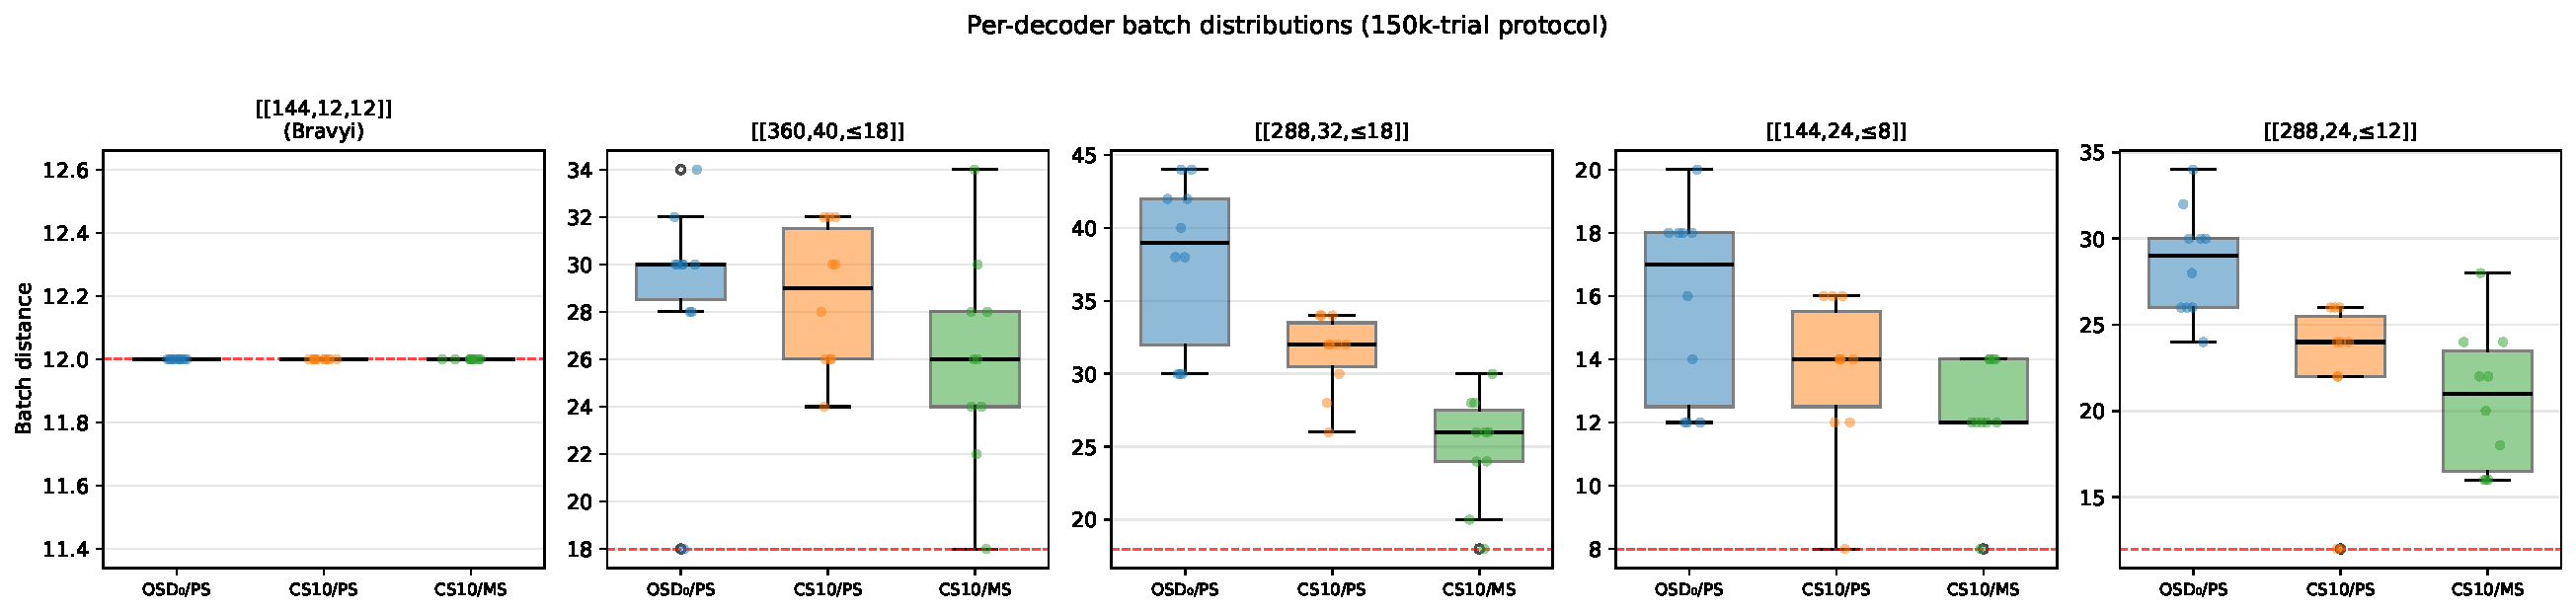
\includegraphics[width=\textwidth]{figures/per_batch_by_decoder.pdf}
\caption{Per-batch distance distributions under the 150{,}000-trial multi-decoder protocol.
Red dashed lines show the global minimum across all 30~batches.
The gross code ($k = 12$) is perfectly stable; all four higher-$k$ codes show inter-batch variance.
The three evolution-highlighted codes ($d_{\text{MILP}} = 2, 4, 6$) show dramatic overestimation; even the $\code{288,24,12}$ ($d_{\text{MILP}} = 12$; a direct sum of two gross codes) has OSD$_0$ medians $\approx 2.4\times$ the true distance, with only 2 of 30 batches finding the exact value.}
\label{fig:sm_per_batch}
\end{figure*}

\subsection{Per-batch statistics}

Table~\ref{tab:per_batch_stats} reports the full per-batch statistics for five representative codes under a second independent 150{,}000-trial run.
MILP exact distances are: $d = 2$ for $\code{360,40}$ at $(15,12)$, $d = 4$ for $\code{288,32}$ at $(24,6)$, $d = 6$ for $\code{144,24}$ at $(12,6)$, $d = 12$ for $\code{288,24}$ at $(12,12)$, and $d = 12$ for the gross code.

\begin{table*}[t]
\centering
\caption{Per-batch distance statistics under the 150{,}000-trial protocol (second independent run).
Each row reports 10~independent batches of 5{,}000 trials per decoder configuration.
Q1/Med/Q3 = 25th/50th/75th percentiles.
The gross code shows perfect stability; high-$k$ codes show dramatic overestimation vs.\ MILP exact distances.}
\label{tab:per_batch_stats}
\small
\begin{tabular}{llcccccc}
\toprule
Code & Decoder & Min & Q1 & Med & Q3 & Max & Mean $\pm$ Std \\
\midrule
\multirow{3}{*}{$\code{144,12,12}$~\cite{bravyi2024high}}
  & OSD$_0$/PS    & 12 & 12 & 12 & 12 & 12 & $12.0 \pm 0.0$ \\
  & CS$_{10}$/PS  & 12 & 12 & 12 & 12 & 12 & $12.0 \pm 0.0$ \\
  & CS$_{10}$/MS  & 12 & 12 & 12 & 12 & 12 & $12.0 \pm 0.0$ \\
\midrule
\multirow{3}{*}{$\code{360,40,2}$}
  & OSD$_0$/PS    & 18 & 28 & 30 & 30 & 34 & $29.0 \pm 4.0$ \\
  & CS$_{10}$/PS  & 24 & 26 & 29 & 31 & 32 & $28.6 \pm 2.8$ \\
  & CS$_{10}$/MS  & 18 & 24 & 26 & 28 & 34 & $26.0 \pm 4.2$ \\
\midrule
\multirow{3}{*}{$\code{288,32,4}$}
  & OSD$_0$/PS    & 30 & 32 & 39 & 42 & 44 & $37.8 \pm 5.5$ \\
  & CS$_{10}$/PS  & 26 & 30 & 32 & 33 & 34 & $31.4 \pm 2.5$ \\
  & CS$_{10}$/MS  & 18 & 24 & 26 & 27 & 30 & $25.0 \pm 3.5$ \\
\midrule
\multirow{3}{*}{$\code{144,24,6}$}
  & OSD$_0$/PS    & 12 & 12 & 17 & 18 & 20 & $15.8 \pm 2.9$ \\
  & CS$_{10}$/PS  &  8 & 12 & 14 & 15 & 16 & $13.6 \pm 2.3$ \\
  & CS$_{10}$/MS  &  8 & 12 & 12 & 14 & 14 & $12.4 \pm 1.7$ \\
\midrule
\multirow{3}{*}{$\code{288,24,12}$}
  & OSD$_0$/PS    & 24 & 26 & 29 & 30 & 34 & $28.6 \pm 3.0$ \\
  & CS$_{10}$/PS  & 12 & 22 & 24 & 25 & 26 & $21.8 \pm 5.1$ \\
  & CS$_{10}$/MS  & 16 & 16 & 21 & 23 & 28 & $20.6 \pm 3.9$ \\
\bottomrule
\end{tabular}
\end{table*}

\subsection{Extended verification at 1{,}500{,}000 trials}

To stress-test the 150k-trial bounds, we ran an extended protocol at $10\times$ depth: 3~decoders $\times$ 10~batches $\times$ 50{,}000~trials $= 1{,}500{,}000$ total trials per code, on three headline codes plus the gross code as a control (Table~\ref{tab:extended}).

\begin{table*}[h]
\centering
\caption{Extended verification at 1{,}500{,}000 trials per code, with MILP exact distances for comparison.
$d_{150\text{k}}$: 150k-trial protocol bound.
$d_{1.5\text{M}}$: extended bound.
$d_{\text{MILP}}$: exact distance via MILP.
Even at $10\times$ depth, BP-OSD overestimates persist.
The $\code{144,32,2}$ code has $A = B$; its $d = 2$ is proven exactly (main text Appendix~D, Theorem~1).}
\label{tab:extended}
\footnotesize
\begin{tabular}{lccccccc}
\toprule
Code & $(\ell,m)$ & $k$ & $d_{150\text{k}}$ & $d_{1.5\text{M}}$ & $d_{\text{MILP}}$ & Batches & $\FOM_{\text{MILP}}$ \\
\midrule
$\code{144,12,12}$ & $(12,6)$ & 12 & 12 & 12 & 12 & 30/30 & 12.0 \\
$\code{360,40,2}$ & $(15,12)$ & 40 & 24 & 6 & 2 & 1/30 & 0.4 \\
$\code{288,32,4}$ & $(24,6)$ & 32 & 22 & 12 & 4 & 1/30 & 1.8 \\
$\code{144,32,2}$ & $(12,6)$ & 32 & 14 & 2 & 2 & 1/30 & 0.9 \\
\bottomrule
\end{tabular}
\end{table*}

The gross code returned $d = 12$ in every batch, confirming that low-rate codes have stable BP-OSD bounds.
All three high-$k$ codes had bounds tightened: $d \leq 6$ for $\code{360,40}$ (MILP: $d = 2$), $d \leq 12$ for $\code{288,32}$ (MILP: $d = 4$), and $d = 2$ for $\code{144,32}$ (MILP: $d = 2$, proven exactly by main text Appendix~D, Theorem~1).
The $10\times$ deeper protocol correctly identified the \emph{direction} of the bias but still overestimated true distances by $3\times$, demonstrating that even million-trial BP-OSD protocols cannot substitute for exact distance computation.

The $d = 2$ result for the $A = B$ code is now \emph{proven exact}: all BB codes with $A = B$ and $k > 0$ have $d = 2$, because the identical column blocks of $H_Z = [A^\top | A^\top]$ produce $\ell m$ weight-2 vectors in $\ker(H_Z)$, exactly $k/2$ of which are independent nontrivial logicals.
The fact that 29 of 30 batches \emph{failed} to find this weight-2 logical---despite 72~independent weight-2 logicals existing---is a cautionary demonstration of BP-OSD's unreliability.

%% =====================================================================
\section{Distance tightening across Campaigns~1--3}
\label{sm:tightening}

Table~\ref{tab:decoder_comparison_full} shows representative distance tightening examples from the Campaign~1 codes when moving from 60{,}000 to 150{,}000 trials under the multi-decoder protocol.
This data supplements Fig.~4 in the main text.

\begin{table*}[t]
\centering
\caption{Impact of verification protocol rigor on distance bounds (Campaign~1 codes).
$\Delta d$ is the reduction in the distance upper bound.
MILP exact distances confirm that even the 150k bounds are gross overestimates.}
\label{tab:decoder_comparison_full}
\begin{tabular}{lcccr}
\toprule
Code & $d_{\leq}$ (60k) & $d_{\leq}$ (150k) & $\Delta d$ & $\Delta\FOM_{\text{BP}}$ \\
\midrule
$\code{360,40}$ & 20 & 20 & 0 & 0.0 \\
$\code{360,32}$ & 20 & 16 & $-4$ & $-12.8$ \\
$\code{288,24}$ & 20 & 12 & $-8$ & $-21.3$ \\
$\code{288,32}$ & 16 & 12 & $-4$ & $-12.4$ \\
$\code{144,24}$ & 12 & 8 & $-4$ & $-13.3$ \\
$\code{144,32}$ & 10 & 6 & $-4$ & $-14.2$ \\
$\code{360,32}$ & 16 & 8 & $-8$ & $-17.1$ \\
$\code{288,32}$ & 24 & 20 & $-4$ & $-19.6$ \\
$\code{288,32}$ & 14 & 10 & $-4$ & $-10.7$ \\
\bottomrule
\end{tabular}
\end{table*}

%% =====================================================================
\section{Univariate code families}
\label{sm:univariate}

Table~\ref{tab:uv_families} lists the top univariate (HGP of low-distance cyclic codes~\cite{eberhardt2024pruning}) polynomial families identified across all campaigns, showing how the same polynomial pair yields different parameters at different lattice dimensions.
Of the 154 Campaigns~1--3 trinomial representations, 87 (57\%) are univariate; after BLISS deduplication, these correspond to 12 distinct codes.
Multiple univariate families achieve $k = 40$ (the highest among trinomial codes; Campaign~4's mixed-monomial codes reach $k = 54$ via a factored-product generalization).
MILP exact distance computation reveals that \emph{every} univariate code has $d \in \{2, 4\}$.
By the Tillich--Z\'emor formula $d = \min(d_1, d_2, d_1^\top, d_2^\top)$~\cite{tillich2014quantum}, the BB distance is bounded by the smallest distance among the four component cyclic codes $\ker H_A$, $\ker H_B$, $\ker H_A^\top$, $\ker H_B^\top$ (for palindromic check polynomials as here, $H^\top = H$, so the four-way min collapses to $\min(d_A, d_B)$); low-weight quotients $(y^m{-}1)/A$ or $(x^\ell{-}1)/B$ force this min to be small (typically 2 or 4), and the odd weight of trinomial check polynomials forces all four component distances to be even, ruling out $d = 3$.
See main text Sec.~VI\,A for the derivation.
The FOM collapse is dramatic: the top-ranked code drops from $\FOM_{\text{BP}} = 64.0$ to $\FOM_{\text{MILP}} = 0.4$.

\begin{table*}[t]
\centering
\caption{Top univariate families ($A = f(y)$, $B = g(x)$, or vice versa; equivalent to HGP of low-distance cyclic codes~\cite{eberhardt2024pruning}).
Rows grouped by polynomial pair; sorted by $\FOM_{\text{BP}}$ descending (the metric available during evolution).
All univariate codes have $d_{\text{MILP}} \leq 4$, regardless of BP-OSD estimate (up to $12\times$ overestimation).}
\label{tab:uv_families}
\begin{tabular}{llccccccccc}
\toprule
$A(y)$ & $B(x)$ & $(\ell,m)$ & $n$ & $k$ & $d_{\text{MILP}}$ & $\FOM_{\text{MILP}}$ & $d_{\text{BP}}$ & $\FOM_{\text{BP}}$ & Ratio \\
\midrule
$1{+}y^{10}{+}y^{11}$ & $1{+}x^{5}{+}x^{10}$ & $(15,12)$ & 360 & 40 & 2 & 0.4 & 24 & 64.0 & 12$\times$ \\
\midrule
$1{+}y{+}y^{2}$ & $1{+}x^{5}{+}x^{25}$ & $(30,6)$ & 360 & 40 & 4 & 1.8 & 24 & 64.0 & 6$\times$ \\
\midrule
$1{+}y^{2}{+}y^{7}$ & $1{+}x^{5}{+}x^{10}$ & $(15,12)$ & 360 & 40 & 2 & 0.4 & 22 & 53.8 & 11$\times$ \\
\midrule
$1{+}y{+}y^{2}$ & $1{+}x^{5}{+}x^{10}$ & $(15,12)$ & 360 & 40 & 2 & 0.4 & 20 & 44.4 & 10$\times$ \\
 & & $(30,6)$ & 360 & 40 & 4 & 1.8 & 20 & 44.4 & 5$\times$ \\
\midrule
$1{+}y{+}y^{2}$ & $1{+}x^{20}{+}x^{25}$ & $(30,6)$ & 360 & 40 & 4 & 1.8 & 20 & 44.4 & 5$\times$ \\
\midrule
$1{+}y{+}y^{5}$ & $1{+}x^{5}{+}x^{10}$ & $(15,12)$ & 360 & 40 & 2 & 0.4 & 18 & 36.0 & 9$\times$ \\
 & & $(30,6)$ & 360 & 40 & 4 & 1.8 & 20 & 44.4 & 5$\times$ \\
\midrule
$1{+}y^{4}{+}y^{5}$ & $1{+}x^{5}{+}x^{10}$ & $(15,12)$ & 360 & 40 & 2 & 0.4 & 20 & 44.4 & 10$\times$ \\
 & & $(30,6)$ & 360 & 40 & 4 & 1.8 & 20 & 44.4 & 5$\times$ \\
\midrule
$1{+}y^{4}{+}y^{5}$ & $1{+}x^{20}{+}x^{25}$ & $(30,6)$ & 360 & 40 & 4 & 1.8 & 20 & 44.4 & 5$\times$ \\
\midrule
$1{+}y{+}y^{5}$ & $1{+}x^{5}{+}x^{25}$ & $(30,6)$ & 360 & 40 & 4 & 1.8 & 20 & 44.4 & 5$\times$ \\
\midrule
$1{+}y{+}y^{11}$ & $1{+}x^{5}{+}x^{10}$ & $(15,12)$ & 360 & 40 & 2 & 0.4 & 18 & 36.0 & 9$\times$ \\
\midrule
$1{+}y^{4}{+}y^{11}$ & $1{+}x^{5}{+}x^{10}$ & $(15,12)$ & 360 & 40 & 2 & 0.4 & 18 & 36.0 & 9$\times$ \\
\midrule
$1{+}y{+}y^{2}$ & $1{+}x^{4}{+}x^{18}$ & $(30,6)$ & 360 & 32 & 4 & 1.4 & 20 & 35.6 & 5$\times$ \\
\midrule
$1{+}y^{2}{+}y^{4}$ & $1{+}x^{16}{+}x^{19}$ & $(30,6)$ & 360 & 32 & 2 & 0.4 & 20 & 35.6 & 10$\times$ \\
\midrule
$1{+}y{+}y^{5}$ & $1{+}x^{4}{+}x^{8}$ & $(12,6)$ & 144 & 32 & 2 & 0.9 & 12 & 32.0 & 6$\times$ \\
 & & $(12,12)$ & 288 & 32 & 2 & 0.4 & 14 & 21.8 & 7$\times$ \\
 & & $(24,6)$ & 288 & 32 & 4 & 1.8 & 12 & 16.0 & 3$\times$ \\
\midrule
$1{+}y{+}y^{2}$ & $1{+}x^{4}{+}x^{8}$ & $(12,6)$ & 144 & 32 & 2 & 0.9 & 6 & 8.0 & 3$\times$ \\
 & & $(12,12)$ & 288 & 32 & 2 & 0.4 & 12 & 16.0 & 6$\times$ \\
 & & $(24,6)$ & 288 & 32 & 4 & 1.8 & 16 & 28.4 & 4$\times$ \\
\midrule
$1{+}y^{8}{+}y^{10}$ & $1{+}x^{2}{+}x^{4}$ & $(6,12)$ & 144 & 32 & 2 & 0.9 & 6 & 8.0 & 3$\times$ \\
 & & $(12,12)$ & 288 & 32 & 4 & 1.8 & 16 & 28.4 & 4$\times$ \\
\midrule
$1{+}y{+}y^{5}$ & $1{+}x^{4}{+}x^{20}$ & $(24,6)$ & 288 & 32 & 4 & 1.8 & 16 & 28.4 & 4$\times$ \\
\midrule
$1{+}y{+}y^{2}$ & $1{+}x^{16}{+}x^{20}$ & $(24,6)$ & 288 & 32 & 4 & 1.8 & 16 & 28.4 & 4$\times$ \\
\midrule
$1{+}y^{5}{+}y^{10}$ & $1{+}x^{5}{+}x^{10}$ & $(15,12)$ & 360 & 40 & 2 & 0.4 & 16 & 28.4 & 8$\times$ \\
\midrule
$1{+}y^{7}{+}y^{11}$ & $1{+}x^{5}{+}x^{10}$ & $(15,12)$ & 360 & 40 & 2 & 0.4 & 16 & 28.4 & 8$\times$ \\
\bottomrule
\end{tabular}
\end{table*}

%% =====================================================================
\section{Full code capacity simulation data}
\label{sm:threshold}

This section presents the complete numerical results of the code capacity simulation summarized in the main text (Sec.~VI\,D).
Tables~\ref{tab:threshold_full} and~\ref{tab:per_qubit_full} cover six CSS codes (five weight-6 BB and one weight-8) at all 12 tested error rates; Table~\ref{tab:threshold_full_extra} adds two additional CSS codes ($\code{288,50,8}$ and $\code{144,8,12}$).
Tables~\ref{tab:threshold_noncss_full} and~\ref{tab:per_qubit_noncss_full} cover five non-CSS PBB codes alongside the CSS gross code baseline under $X$-only noise.
Table~\ref{tab:threshold_depolarizing_full} presents the same non-CSS codes under depolarizing noise; the table caption notes the decoder configuration and that, like the main text Sec.~VI\,D depolarizing data, this is a decoder-mismatched threshold (iid X/Z BP-OSD prior on the depolarizing channel) rather than the optimal depolarizing threshold.

\paragraph{Simulation protocol.}
Two noise channels are simulated with separate decoder configurations.
For the X-only tables (Tables~\ref{tab:threshold_full}--\ref{tab:per_qubit_noncss_full}): independent $X$ errors at rate~$p$ on each of~$n$ qubits, decoded with BP-OSD on $H_z$ with an iid prior of marginal rate~$p$ on $n$ columns.
For Table~\ref{tab:threshold_depolarizing_full}: the depolarizing channel (each qubit independently gets $X$, $Y$, or $Z$ with probability $p/3$), decoded with BP-OSD on the symplectic check matrix $[H_z \mid H_x]$ with iid bit-flip priors at marginal rate $2p/3$ on each of the $2n$ columns.
This iid prior is mismatched with respect to the depolarizing channel (it does not model the $X$/$Z$ correlation $P(e_x{=}1, e_z{=}1) = p/3$ induced by $Y$ errors); see main text Sec.~VI\,D and the table caption.
All decoders use OSD-CS order~7, product-sum, 20~BP iterations~\cite{panteleev2021degenerate,roffe2020decoding}.
Block LER: fraction of 100{,}000 shots with $\geq 1$ logical error among $k$~qubits.
Per-logical-qubit rate: $p_L = 1 - (1 - \text{LER})^{1/k}$.
Wilson 95\% CIs $\leq 0.06$~pp for LER~$\leq 1\%$; entries reported as $0.00$ have upper bounds $< 0.01\%$.

\begin{table*}[t]
\centering
\caption{Code capacity simulation: block logical error rate (LER, \%) vs.\ physical error rate~$p$ for six CSS codes (five weight-6 BB and one weight-8$^\dagger$; 100{,}000 shots per point).
Bold entries indicate block LER~$> p$.
$^\dagger$Campaign~4 code (weight-8 stabilizers; MILP incumbent $d \leq 14$; BP-OSD 300k confirms $d = 14$).
See Table~\ref{tab:threshold_full_extra} for two additional CSS codes.}
\label{tab:threshold_full}
\small
\begin{tabular}{r|cc|cc|cc|cc|cc|cc}
\toprule
& \multicolumn{2}{c|}{$\code{144,12,12}$~\cite{bravyi2024high}} & \multicolumn{2}{c|}{$\code{288,24,12}$} & \multicolumn{2}{c|}{$\code{288,16,12}$} & \multicolumn{2}{c|}{$\code{360,16,{\leq}14}$} & \multicolumn{2}{c|}{$\code{360,20,{\leq}14}$$^\dagger$} & \multicolumn{2}{c}{$\code{144,24,6}$} \\
$p$ (\%) & LER & Unc. & LER & Unc. & LER & Unc. & LER & Unc. & LER & Unc. & LER & Unc. \\
\midrule
0.2 & 0.00 & 2.37 & 0.00 & 4.69 & 0.00 & 3.15 & 0.00 & 3.15 & 0.00 & 3.92 & 0.00 & 4.69 \\
0.5 & 0.00 & 5.84 & 0.01 & 11.33 & 0.01 & 7.71 & 0.01 & 7.71 & 0.00 & 9.54 & 0.02 & 11.33 \\
0.8 & 0.01 & 9.19 & 0.04 & 17.53 & 0.08 & 12.06 & 0.07 & 12.06 & 0.01 & 14.84 & 0.10 & 17.53 \\
1.0 & 0.03 & 11.36 & 0.07 & 21.43 & 0.13 & 14.85 & 0.15 & 14.85 & 0.02 & 18.21 & 0.27 & 21.43 \\
1.5 & 0.08 & 16.59 & 0.19 & 30.42 & 0.41 & 21.48 & 0.43 & 21.48 & 0.04 & 26.09 & 0.85 & 30.42 \\
2.0 & 0.15 & 21.53 & 0.36 & 38.42 & 0.85 & 27.62 & 0.84 & 27.62 & 0.12 & 33.24 & \textbf{2.11} & 38.42 \\
3.0 & 0.49 & 30.62 & 0.98 & 51.86 & 1.69 & 38.57 & 1.69 & 38.57 & 0.60 & 45.62 & \textbf{7.22} & 51.86 \\
4.0 & 1.28 & 38.73 & 2.66 & 62.46 & 2.55 & 47.96 & 2.98 & 47.96 & 2.38 & 55.80 & \textbf{16.77} & 62.46 \\
5.0 & 3.70 & 45.96 & \textbf{7.28} & 70.80 & 4.18 & 55.99 & \textbf{5.27} & 55.99 & \textbf{7.95} & 64.15 & \textbf{28.97} & 70.80 \\
6.0 & \textbf{8.61} & 52.41 & \textbf{16.77} & 77.35 & \textbf{7.45} & 62.84 & \textbf{10.99} & 62.84 & \textbf{20.10} & 70.99 & \textbf{43.56} & 77.35 \\
7.0 & \textbf{16.99} & 58.14 & \textbf{31.69} & 82.48 & \textbf{14.66} & 68.69 & \textbf{21.95} & 68.69 & \textbf{38.50} & 76.58 & \textbf{57.89} & 82.48 \\
8.0 & \textbf{28.76} & 63.23 & \textbf{50.06} & 86.48 & \textbf{27.73} & 73.66 & \textbf{38.70} & 73.66 & \textbf{60.29} & 81.13 & \textbf{70.68} & 86.48 \\
\bottomrule
\end{tabular}
\end{table*}

\begin{table*}[t]
\centering
\caption{Per-logical-qubit error rate $p_L = 1{-}(1{-}\text{LER})^{1/k}$ (\%) for the six CSS codes in Table~\ref{tab:threshold_full}.
All six codes achieve $p_L < p$ at every tested rate, confirming genuine per-qubit error suppression.
$^\dagger$Campaign~4 code (weight-8 stabilizers).}
\label{tab:per_qubit_full}
\footnotesize
\begin{tabular}{r|c|c|c|c|c|c}
\toprule
$p$ (\%) & $\code{144,12,12}$ ($k{=}12$) & $\code{288,24,12}$ ($k{=}24$) & $\code{288,16,12}$ ($k{=}16$) & $\code{360,16,{\leq}14}$ ($k{=}16$) & $\code{360,20,{\leq}14}$$^\dagger$ ($k{=}20$) & $\code{144,24,6}$ ($k{=}24$) \\
\midrule
0.2 & ${<}0.01$ & ${<}0.01$ & ${<}0.01$ & ${<}0.01$ & ${<}0.01$ & ${<}0.01$ \\
0.5 & ${<}0.01$ & ${<}0.01$ & ${<}0.01$ & ${<}0.01$ & ${<}0.01$ & ${<}0.01$ \\
0.8 & ${<}0.01$ & ${<}0.01$ & ${<}0.01$ & ${<}0.01$ & ${<}0.01$ & ${<}0.01$ \\
1.0 & ${<}0.01$ & ${<}0.01$ & 0.01 & 0.01 & ${<}0.01$ & 0.01 \\
1.5 & 0.01 & 0.01 & 0.03 & 0.03 & ${<}0.01$ & 0.04 \\
2.0 & 0.01 & 0.01 & 0.05 & 0.05 & 0.01 & 0.09 \\
3.0 & 0.04 & 0.04 & 0.11 & 0.11 & 0.03 & 0.31 \\
4.0 & 0.11 & 0.11 & 0.16 & 0.19 & 0.12 & 0.76 \\
5.0 & 0.31 & 0.31 & 0.27 & 0.34 & 0.41 & 1.42 \\
6.0 & 0.75 & 0.76 & 0.48 & 0.73 & 1.12 & 2.35 \\
7.0 & 1.54 & 1.58 & 0.99 & 1.54 & 2.40 & 3.54 \\
8.0 & 2.79 & 2.85 & 2.01 & 3.01 & 4.51 & 4.98 \\
\bottomrule
\end{tabular}
\end{table*}

\begin{table*}[t]
\centering
\caption{Code capacity simulation: block LER (\%) and per-logical-qubit rate $p_L$ (\%) for two additional CSS codes (100{,}000 shots per point).
Bold entries indicate block LER~$> p$.
$^\ddagger$Campaign~4 code (weight-8 stabilizers, cross-factored).}
\label{tab:threshold_full_extra}
\small
\begin{tabular}{r|ccc|ccc}
\toprule
& \multicolumn{3}{c|}{$\code{288,50,8}^{\ddagger}$} & \multicolumn{3}{c}{$\code{144,8,12}$} \\
$p$ (\%) & LER & $p_L$ & Unc. & LER & $p_L$ & Unc. \\
\midrule
0.2 & 0.00 & ${<}0.01$ & 9.53 & 0.00 & ${<}0.01$ & 1.59 \\
0.5 & 0.02 & ${<}0.01$ & 22.17 & 0.00 & ${<}0.01$ & 3.93 \\
0.8 & 0.08 & ${<}0.01$ & 33.08 & 0.01 & ${<}0.01$ & 6.22 \\
1.0 & 0.13 & ${<}0.01$ & 39.50 & 0.01 & ${<}0.01$ & 7.73 \\
1.5 & 0.48 & 0.01 & 53.03 & 0.05 & 0.01 & 11.39 \\
2.0 & 1.22 & 0.02 & 63.58 & 0.08 & 0.01 & 14.92 \\
3.0 & \textbf{4.71} & 0.10 & 78.19 & 0.29 & 0.04 & 21.63 \\
4.0 & \textbf{12.74} & 0.27 & 87.01 & 0.91 & 0.11 & 27.86 \\
5.0 & \textbf{27.20} & 0.63 & 92.31 & 2.72 & 0.34 & 33.66 \\
6.0 & \textbf{46.27} & 1.23 & 95.47 & \textbf{6.44} & 0.83 & 39.04 \\
7.0 & \textbf{65.92} & 2.13 & 97.34 & \textbf{13.13} & 1.74 & 44.04 \\
8.0 & \textbf{81.28} & 3.30 & 98.45 & \textbf{23.07} & 3.23 & 48.68 \\
\bottomrule
\end{tabular}
\end{table*}

\begin{table*}[t]
\centering
\caption{Code capacity simulation ($X$-only noise): block LER (\%) for five non-CSS PBB codes and the CSS gross code baseline (100{,}000 shots).
Bold entries indicate block LER~$> p$.}
\label{tab:threshold_noncss_full}
\small
\setlength{\tabcolsep}{3pt}
\begin{tabular}{r|cc|cc|cc|cc|cc|cc}
\toprule
& \multicolumn{2}{c|}{$\code{144,12,12}$~\cite{bravyi2024high} (CSS)} & \multicolumn{2}{c|}{$\code{144,12,12}$ PBB} & \multicolumn{2}{c|}{$\code{72,4,8}$ PBB} & \multicolumn{2}{c|}{$\code{108,8,10}$ PBB} & \multicolumn{2}{c|}{$\code{360,12,{\leq}20}$ PBB} & \multicolumn{2}{c}{$\code{360,12,{\leq}24}$ PBB} \\
$p$ (\%) & LER & Unc. & LER & Unc. & LER & Unc. & LER & Unc. & LER & Unc. & LER & Unc. \\
\midrule
0.2 & 0.00 & 2.37 & 0.00 & 2.37 & 0.00 & 0.80 & 0.00 & 1.59 & 0.00 & 2.37 & 0.00 & 2.37 \\
0.5 & 0.00 & 5.84 & 0.01 & 5.84 & 0.00 & 1.99 & 0.00 & 3.93 & 0.00 & 5.84 & 0.00 & 5.84 \\
0.8 & 0.01 & 9.19 & 0.01 & 9.19 & 0.00 & 3.16 & 0.00 & 6.22 & 0.00 & 9.19 & 0.00 & 9.19 \\
1.0 & 0.03 & 11.36 & 0.02 & 11.36 & 0.00 & 3.94 & 0.00 & 7.73 & 0.00 & 11.36 & 0.00 & 11.36 \\
1.5 & 0.08 & 16.59 & 0.08 & 16.59 & 0.00 & 5.87 & 0.00 & 11.39 & 0.00 & 16.59 & 0.00 & 16.59 \\
2.0 & 0.15 & 21.53 & 0.21 & 21.53 & 0.00 & 7.76 & 0.00 & 14.92 & 0.00 & 21.53 & 0.00 & 21.53 \\
3.0 & 0.49 & 30.62 & 0.76 & 30.62 & 0.01 & 11.47 & 0.01 & 21.63 & 0.00 & 30.62 & 0.01 & 30.62 \\
4.0 & 1.28 & 38.73 & 2.07 & 38.73 & 0.02 & 15.07 & 0.02 & 27.86 & 0.01 & 38.73 & 0.02 & 38.73 \\
5.0 & 3.70 & 45.96 & 4.29 & 45.96 & 0.04 & 18.55 & 0.05 & 33.66 & 0.04 & 45.96 & 0.04 & 45.96 \\
6.0 & \textbf{8.61} & 52.41 & \textbf{7.51} & 52.41 & 0.07 & 21.93 & 0.12 & 39.04 & 0.15 & 52.41 & 0.16 & 52.41 \\
7.0 & \textbf{16.99} & 58.14 & \textbf{11.64} & 58.14 & 0.15 & 25.19 & 0.25 & 44.04 & 0.39 & 58.14 & 0.37 & 58.14 \\
8.0 & \textbf{28.76} & 63.23 & \textbf{16.61} & 63.23 & 0.22 & 28.36 & 0.51 & 48.68 & 0.93 & 63.23 & 0.90 & 63.23 \\
\bottomrule
\end{tabular}
\end{table*}

\begin{table*}[t]
\centering
\caption{Per-logical-qubit error rate $p_L = 1{-}(1{-}\text{LER})^{1/k}$ (\%) for the non-CSS PBB codes in Table~\ref{tab:threshold_noncss_full} ($X$-only noise).
All six codes achieve $p_L < p$ at every tested rate.
The two $n=360$ codes have identical per-qubit rates at displayed precision since both have $k=12$ and their $X$-only LER values agree to within rounding.}
\label{tab:per_qubit_noncss_full}
\tiny
\setlength{\tabcolsep}{2pt}
\begin{tabular}{r|c|c|c|c|c|c}
\toprule
$p$ (\%) & $\code{144,12,12}$ CSS ($k{=}12$) & $\code{144,12,12}$ PBB ($k{=}12$) & $\code{72,4,8}$ PBB ($k{=}4$) & $\code{108,8,10}$ PBB ($k{=}8$) & $\code{360,12,{\leq}20}$ PBB ($k{=}12$) & $\code{360,12,{\leq}24}$ PBB ($k{=}12$) \\
\midrule
0.2 & ${<}0.01$ & ${<}0.01$ & ${<}0.01$ & ${<}0.01$ & ${<}0.01$ & ${<}0.01$ \\
0.5 & ${<}0.01$ & ${<}0.01$ & ${<}0.01$ & ${<}0.01$ & ${<}0.01$ & ${<}0.01$ \\
0.8 & ${<}0.01$ & ${<}0.01$ & ${<}0.01$ & ${<}0.01$ & ${<}0.01$ & ${<}0.01$ \\
1.0 & ${<}0.01$ & ${<}0.01$ & ${<}0.01$ & ${<}0.01$ & ${<}0.01$ & ${<}0.01$ \\
1.5 & 0.01 & 0.01 & ${<}0.01$ & ${<}0.01$ & ${<}0.01$ & ${<}0.01$ \\
2.0 & 0.01 & 0.02 & ${<}0.01$ & ${<}0.01$ & ${<}0.01$ & ${<}0.01$ \\
3.0 & 0.04 & 0.06 & ${<}0.01$ & ${<}0.01$ & ${<}0.01$ & ${<}0.01$ \\
4.0 & 0.11 & 0.17 & ${<}0.01$ & ${<}0.01$ & ${<}0.01$ & ${<}0.01$ \\
5.0 & 0.31 & 0.36 & 0.01 & 0.01 & ${<}0.01$ & ${<}0.01$ \\
6.0 & 0.75 & 0.65 & 0.02 & 0.01 & 0.01 & 0.01 \\
7.0 & 1.54 & 1.03 & 0.04 & 0.03 & 0.03 & 0.03 \\
8.0 & 2.79 & 1.50 & 0.06 & 0.06 & 0.08 & 0.08 \\
\bottomrule
\end{tabular}
\end{table*}

\begin{table*}[t]
\centering
\caption{Code capacity simulation (depolarizing channel, decoded with iid X/Z BP-OSD prior): block LER (\%) for five non-CSS PBB codes and the CSS gross code baseline (100{,}000 shots).
Sampler: each qubit independently gets $X$, $Y$, or $Z$ with probability $p/3$.
Decoder: BP-OSD on the symplectic check matrix $[H_z \mid H_x]$ with iid bit-flip priors at marginal rate $2p/3$ on each of the $2n$ columns; this iid prior is mismatched with respect to the depolarizing channel (see main text Sec.~VI\,D), so the reported LERs are a lower bound on the optimal depolarizing threshold rather than the optimal threshold itself.
Bold entries indicate block LER~$> p$.
Under depolarizing noise, the CSS and PBB $\code{144,12,12}$ achieve nearly identical LER at all tested rates---a comparison that is decoder-dependent.
Both $n=360$ PBB codes achieve LER~$<p$ throughout: the top-FOM $\code{360,12,{\leq}24}$ reaches $4.52\%$ and the lower-FOM $\code{360,12,{\leq}20}$ reaches $4.97\%$ at $p=8\%$, with a small crossover in which the lower-FOM code is marginally better at low $p$ ($p \leq 4\%$) and the higher-FOM code is better at high $p$ ($p \geq 5\%$).}
\label{tab:threshold_depolarizing_full}
\small
\setlength{\tabcolsep}{3pt}
\begin{tabular}{r|cc|cc|cc|cc|cc|cc}
\toprule
& \multicolumn{2}{c|}{$\code{144,12,12}$~\cite{bravyi2024high} (CSS)} & \multicolumn{2}{c|}{$\code{144,12,12}$ PBB} & \multicolumn{2}{c|}{$\code{72,4,8}$ PBB} & \multicolumn{2}{c|}{$\code{108,8,10}$ PBB} & \multicolumn{2}{c|}{$\code{360,12,{\leq}20}$ PBB} & \multicolumn{2}{c}{$\code{360,12,{\leq}24}$ PBB} \\
$p$ (\%) & LER & Unc. & LER & Unc. & LER & Unc. & LER & Unc. & LER & Unc. & LER & Unc. \\
\midrule
0.2 & 0.00 & 2.37 & 0.00 & 2.37 & 0.00 & 0.80 & 0.00 & 1.59 & 0.00 & 2.37 & 0.00 & 2.37 \\
0.5 & 0.00 & 5.84 & 0.01 & 5.84 & 0.00 & 1.99 & 0.00 & 3.93 & 0.00 & 5.84 & 0.01 & 5.84 \\
0.8 & 0.01 & 9.19 & 0.01 & 9.19 & 0.00 & 3.16 & 0.01 & 6.22 & 0.03 & 9.19 & 0.05 & 9.19 \\
1.0 & 0.03 & 11.36 & 0.02 & 11.36 & 0.01 & 3.94 & 0.01 & 7.73 & 0.05 & 11.36 & 0.08 & 11.36 \\
1.5 & 0.09 & 16.59 & 0.07 & 16.59 & 0.01 & 5.87 & 0.03 & 11.39 & 0.15 & 16.59 & 0.19 & 16.59 \\
2.0 & 0.13 & 21.53 & 0.14 & 21.53 & 0.05 & 7.76 & 0.07 & 14.92 & 0.27 & 21.53 & 0.35 & 21.53 \\
3.0 & 0.37 & 30.62 & 0.34 & 30.62 & 0.25 & 11.47 & 0.18 & 21.63 & 0.70 & 30.62 & 0.81 & 30.62 \\
4.0 & 0.71 & 38.73 & 0.67 & 38.73 & 0.69 & 15.07 & 0.49 & 27.86 & 1.24 & 38.73 & 1.27 & 38.73 \\
5.0 & 1.27 & 45.96 & 1.40 & 45.96 & 1.80 & 18.55 & 1.05 & 33.66 & 1.89 & 45.96 & 1.82 & 45.96 \\
6.0 & 2.69 & 52.41 & 2.64 & 52.41 & 3.73 & 21.93 & 2.32 & 39.04 & 2.59 & 52.41 & 2.40 & 52.41 \\
7.0 & 5.15 & 58.14 & 5.22 & 58.14 & 6.63 & 25.19 & 4.56 & 44.04 & 3.58 & 58.14 & 3.22 & 58.14 \\
\textbf{8.0} & \textbf{9.43} & 63.23 & \textbf{9.29} & 63.23 & \textbf{10.47} & 28.36 & \textbf{8.38} & 48.68 & 4.97 & 63.23 & 4.52 & 63.23 \\
\bottomrule
\end{tabular}
\end{table*}

%% =====================================================================
\section{Utility stratification of the catalog}
\label{sm:utility}

Not all 465 distinct codes are useful for error correction.
We stratify the combined catalog by practical relevance.

Among the 97 CSS codes, the MILP-verified distance distribution spans $d = 2$ (the $A = B$ and some univariate codes) through $d = 14$.
Among the Campaigns~1--3 trinomial portion of the catalog, 13 $(n, k, d)$ parameter triples have $d \geq 6$ (the $x/y$-swap and select mixed-monomial families); Campaign~4's mixed-monomial search expands this to 41 distinct triples with $d \geq 6$ across the full CSS catalog.
The CSS codes with $\FOM \geq 6.0$---a threshold above which codes offer meaningful error-correction advantage over the uncoded rate---number 5 parameter triples at Campaigns~1--3 block lengths (including the $\code{288,24,12}$ at $\FOM = 12.0$, which is a direct sum of two gross codes; see main text Sec.~VI\,A) and 29 additional $(n,k,d)$ triples reached only by Campaign~4 (34 distinct CSS triples in total at $\FOM \geq 6$).

In contrast, all 368 non-CSS PBB codes have $d \geq 6$ by construction: Campaign~5's adaptive pipeline rejected $d \leq 4$ codes during evolution.
Of these, 108 distinct codes have $\FOM \geq 6.0$, 53 have $\FOM \geq 8.0$, and 25 match or exceed $\FOM = 12.0$.

The most practically relevant codes---those with $d \geq 8$ and $\FOM \geq 6.0$---span 50 distinct $(n,k,d)$ parameter triples across both catalogs (30 CSS, 24 non-CSS, with 4 shared between the two catalogs); a representative subset is consolidated in main text Table~V.

%% =====================================================================
\section{Additional comparison and novelty details}
\label{sm:comparison}

\subsection{Novelty assessment}
\label{sm:novelty}

The published inventory of weight-6 BB codes at the block lengths we study ($n = 144$, $288$, $360$) is small: one code each from Bravyi et al.~\cite{bravyi2024high}.
Weight-8 codes have been reported at $n = 144$ by Symons et al.~\cite{symons2025covering} ($\code{144,14,14}$, $\FOM = 19.1$, covering graphs) and Liang and Chen~\cite{liang2025selfdual} ($\code{144,6,14}$, $\FOM = 8.2$, self-dual).
Among the most comprehensive systematic searches is Liang et al.~\cite{liang2025generalized}, who enumerate all weight-6 generalized toric codes of a canonical 3-term form $f = 1{+}x{+}x^a y^b$ for $n \leq 400$; at $n = 288$ they report only the $\code{288,12,18}$.
Our $x/y$-swap codes do \emph{not} fall within their canonical form (which requires one monomial to be the identity and a second to be $x$), though a subset may be equivalent under coordinate transformations of the underlying $\ZZ_\ell \times \ZZ_m$ group (e.g., $x \mapsto x^a$ for $a$ coprime to $\ell$, or swapping $x$ and $y$ when $\ell = m$).
Lin and Pryadko~\cite{lin2024abelian} provide a comprehensive enumeration of 2BGA codes (including nonabelian groups) with weight~$\leq 8$ for $n \leq 100$; this database is complementary to ours but does not include the block lengths considered here.

To our knowledge, two of our 99 CSS equivalence classes match previously reported codes: the gross code $\code{144,12,12}$ and the $\code{360,12,{\leq}24}$ (both~\cite{bravyi2024high}; Campaign~4 rediscovered these through mixed-monomial representations).
The remaining 97 classes do not appear in prior work, including all codes at non-standard factorizations---$(18,8)$, $(16,9)$, $(24,6)$ for $n = 288$; $(15,12)$ for $n = 360$---and all high-rate codes with $k \geq 16$ at $n = 288$.

We note that unreported codes may exist in unpublished search databases (e.g., from industrial groups); our novelty claim is based on a review of 25+ papers and 6 public code repositories through March~2026, and we have not had access to unpublished search data.

\subsection{Weight-8 comparison}
\label{sm:weight8}

Weight-8 codes have eight nonzero entries per row of $H_X$ and $H_Z$, compared to six for weight-6 codes.
Under standard depth-optimal syndrome-extraction circuits, this corresponds to eight controlled-NOT (CNOT) layers per syndrome-extraction cycle versus six (a 33\% increase in circuit depth per cycle), placing weight-8 codes in a different hardware-complexity regime.
At $n = 144$, the weight-8 $\code{144,14,14}$~\cite{symons2025covering} achieves $\FOM = 19.1$, $1.6\times$ our highest weight-6 $\FOM = 12.0$.
Whether the FOM advantage compensates for the increased per-cycle depth depends on the noise model and circuit schedule; a full circuit-level comparison is left to future work.

%% =====================================================================
\section{Campaign details}
\label{sm:campaigns}

\subsection{Evolution dynamics}

\paragraph{Campaign~1 (Gemini~3 Flash Preview, 100 iterations, ${\sim}$US\$15 LLM inference).}
The population of 100 programs across 3 islands reached 79 of 100 occupied MAP-Elites niches at convergence.
The highest-scoring program (combined score 327.0) was found at iteration~83, at generation depth~5, growing from 4~strategies and 230~lines (seed) to 7~strategies and 292~lines with the addition of a univariate strategy.
Nine codes were subjected to full verification.

\paragraph{Campaign~2 (3-model ensemble, 251 iterations, ${\sim}$US\$25 LLM inference).}
The seed solution incorporated five Campaign~1 codes into its known-code table.
Nine improvements were recorded over the seed, with the largest gain ($+39.3$ points) at iteration~3.
Highest combined score: 348.6 ($+6.6\%$ over Campaign~1).
Manually stopped after 251 iterations.

\paragraph{Campaign~3 (3-model ensemble, 500 iterations, ${\sim}$US\$50 LLM inference).}
Population 1{,}000 across 5 islands; highest-scoring program (score 354.4) at iteration~462.
The last ${\sim}275$ iterations produced only one marginal improvement ($+1.2\%$), indicating saturation.
145 unique codes not found in Campaign~1.

\paragraph{Campaign~4 (Ansatz, 300 iterations, ${\sim}$US\$47 LLM inference).}
24 parallel evaluation workers on a 64-core server.
All 1{,}188 codes passing evolutionary fitness filters were MILP-verified; top~39 re-verified with extended budgets (3{,}000\,s per logical, 72{,}000\,s total); top~6 subjected to 300{,}000-trial BP-OSD attacks.
45 distinct codes from structural families not present in~\cite{bravyi2024high}.
Campaign~4 independently rediscovered the gross code through six mixed-monomial representations.

\paragraph{Campaign~5 (PBB, 500 iterations, ${\sim}$US\$100 LLM inference).}
352 productive evaluations of 500 total iterations; 18{,}588 candidate 4-tuples evaluated across 7 lattices.
149 PBB catalog entries deep-verified by MILP (timeouts up to 14{,}400\,s per logical, up to a 60-worker pool); 63 exact outcomes, 33 downward distance corrections identified.
The lattice selection was constrained by MILP runtime: the symplectic formulation is ${\sim}4\times$ slower per logical than CSS, limiting practical verification to the $m \leq 6$ lattice set and excluding the larger-$m$ CSS lattices $(12,12)$ and $(15,12)$.

\paragraph{Total cost.}
The five evolutionary campaigns sum to ${\sim}$US\$237 in LLM inference (per-campaign breakdown above) over ${\sim}140$\,h of wall-clock time (sum of the campaign rows in main text Table~I: $5 + 9.5 + 21 + 92 + 11 = 138.5$\,h); this budget includes the in-loop MILP verification performed by each campaign's evaluator, of which Campaign~4's 92\,h itself absorbs ${\sim}20$\,h ($72{,}000$\,s) of top-code re-verification at $3{,}000$\,s per logical.
The headline ${\sim}$US\$400 figure cited in the abstract additionally covers the ablation arms of main text Sec.~VI\,F (random search at $10^3$ and $10^4$/lattice plus the GA/GA-G arms over 5~seeds each, ${\sim}$US\$70 combined) and exploratory/failed runs (re-tries on flaky API responses, abandoned config sweeps, ${\sim}$US\$90); see the caption of main text Table~I for the same itemization.
The Campaign~5 deep MILP audit on 149 PBB catalog entries (timeouts up to $14{,}400$\,s per logical, up to a 60-worker pool on a 64-core server) is a post-evolution verification step run on a separate machine and is reported \emph{on top of} the ${\sim}140$\,h evolution wall-clock figure rather than within it.
Across all components, MILP verification---not LLM inference---is the dominant compute cost.

\subsection{Fitness trajectory}

Figure~\ref{fig:sm_trajectory} shows the fitness trajectories of Campaigns~1--3 (trinomial search).
The $y$-axis shows the combined score: the sum of highest credible $\FOM = kd^2/n$ values across all evaluated lattices, with trust filtering on $d/\sqrt{n}$ (main text Sec.~V\,D).
The combined score uses BP-OSD distance estimates that are severe overestimates for high-$k$ codes; consequently, the fitness trajectory primarily reflects $k$-optimization rather than true FOM improvement.
The deterministic $k$-only metric $\Sigma_k$ (main text Sec.~VI\,F) provides a robust assessment of search effectiveness.

\begin{figure*}[t]
\centering
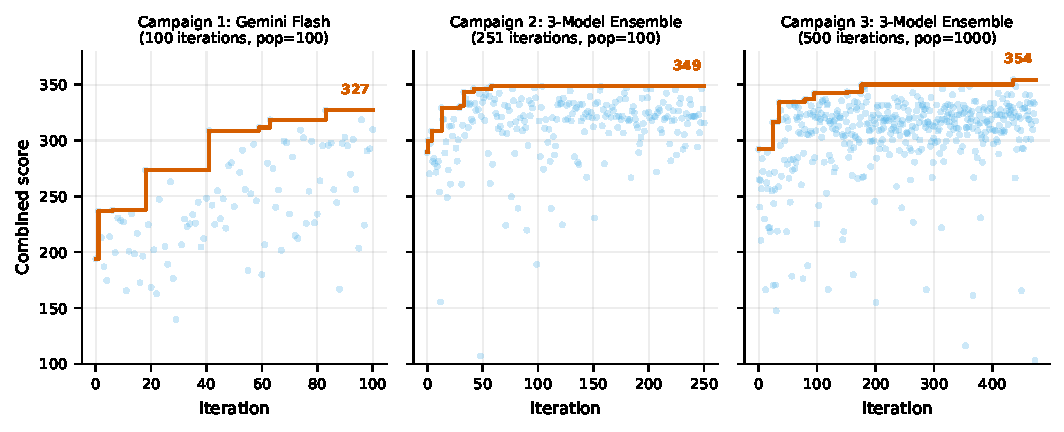
\includegraphics[width=\textwidth]{figures/fig_fitness_trajectory.pdf}
\caption{Fitness trajectories of Campaigns~1--3.
\emph{Left:} Campaign~1 (Gemini~3 Flash, 100 iterations).
\emph{Center:} Campaign~2 (3-model ensemble, 251 iterations, early-stopped).
\emph{Right:} Campaign~3 (3-model ensemble, 500 iterations, population 1{,}000).
Blue dots: per-iteration combined scores; red step line: running maximum.
All campaigns start from the same seed (score~194).
Campaign~3 saturates after ${\sim}225$ iterations.
Campaign~4 used a different evaluation pipeline and is not shown.}
\label{fig:sm_trajectory}
\end{figure*}

\subsection{Cross-campaign analysis}

The ensemble campaigns (2 and 3) collectively produced 145 unique verified codes not found in Campaign~1, including the highest-$k$ trinomial codes: the $\code{360,40,2}$ ($k = 40$), the $\code{288,32,4}$ ($k = 32$), and the $A = B$ $\code{144,32,2}$ ($k = 32$; $d = 2$ by main text Appendix~D, Theorem~1).
Campaign~4's mixed-monomial generalization later surpasses these encoding dimensions, reaching $k = 54$ via factored-product structures.
Campaign~4 added 45 distinct codes from structural families not present in prior catalogs, with only one polynomial-pair overlap with the Campaign~1--3 catalog: the $\code{288,24,12}$ at $(12,12)$.

Campaigns~2--3 differed from Campaign~1 in three dimensions simultaneously: mutation model, iteration count, and population size.
Campaign~2 (ensemble, pop=100, 251 iterations) achieved $\Sigma_k = 464$, \emph{below} Campaign~1's $704$ despite more iterations and model diversity---suggesting that ensemble mutations may produce less focused variation at small population sizes.
Only Campaign~3 (pop=1{,}000, 500 iterations) matched Campaign~1's $\Sigma_k$ and yielded additional codes.
The most parsimonious explanation is that population size and iteration count are the primary drivers; a controlled experiment varying only model configuration would be needed to isolate any ensemble contribution.

%% =====================================================================
\section{Ablation methodology}
\label{sm:ablation}

This section supplements the ablation study presented in the main text (Sec.~VI\,F and Appendix~B) with methodological details.

\paragraph{Arms.}
Eight arms evaluated on the same 8 Stage-2 lattices:
(1) hand-crafted seed generator;
(2) uniform random trinomials at $10^3$/lattice (single seed);
(3) uniform random at $10^4$/lattice (5 independent seeds, 80{,}000 total per seed);
(4) genetic algorithm (GA) with tournament selection (size~5), single-point polynomial crossover, exponent mutation, 10\% elitism, population~200, $10^4$ evaluations per lattice (5~seeds);
(5) GA operating on the same ansatz representation as the LLM (``GA-G''), with abstract syntax tree (AST)-level mutations on integer literals, loop bounds, and strategy blocks, tournament selection (size~5), strategy-block crossover, population~100, 30~generations, ${\sim}2{,}800$ evaluations per seed (5~seeds, ${\sim}14{,}000$ total);
and (6--8) the highest-fitness evolved ansätze from Campaigns~1--3.

\paragraph{GA-G mutation operators.}
The ansatz GA uses six AST-level operators:
(i) changing integer literals ($\pm 1$, $\pm 2$, or random);
(ii) modifying loop bounds;
(iii) duplicating a strategy block with perturbed constants;
(iv) removing a strategy block;
(v) splicing a new strategy from a template library ($x/y$-swap, perturbation, univariate);
(vi) swapping block order.
Crucially, GA-G \emph{cannot} create entirely new strategy branches: it shuffles and parameterizes existing code structure, whereas the LLM can invent qualitatively new patterns from scratch.

\paragraph{Degenerate code verification.}
Exhaustive verification of the exponent-tuple GA across all 5~seeds and 8~lattices (9{,}832 unique codes) confirms that at every lattice where Campaign~1 found codes, every GA code exceeding the per-lattice $\max\{k\}$ has $d \leq 2$ via explicit weight-2 logical operators ($k/n = 2/3$ in all 11~cases).
The per-lattice breakdown: 6~codes at $(12,6)$, 1~at $(6,12)$, 1~at $(12,12)$, and 3~at $(24,6)$.
One of these 11 has $A = B$, for which $d = 2$ is proven; the others share common polynomial factors or other algebraic degeneracies producing $k/n = 2/3$.

At $(16,9)$ and $(18,8)$---where all evolved ansätze fail---the exponent-tuple GA finds genuine $d \geq 3$ codes.
MILP verification of 10 codes with the highest $k$ ($k = 32$--$64$) at these lattices yields $d = 4$--$6$ (all proven exact) and $\FOM \leq 4.0$, a factor of $3$ below the LLM's $\FOM = 12.0$ and below every Bravyi et al.\ baseline.

GA-G reaches $k = n/2$ at six of eight lattices in every seed and at all eight across the union of seeds, producing codes with $d \leq 2$.
Its low variance ($\pm 22$ vs.\ $\pm 142$ for the exponent-tuple GA) reflects rapid convergence to $k = n/2$ attractors within ${\sim}10$ generations.

%% =====================================================================
\section{MILP formulation details}
\label{sm:milp}

\subsection{CSS distance formulation}

Following Bravyi et al.~\cite{bravyi2024high}, we formulate the problem of finding a minimum-weight $X$-type logical operator for the $j$-th logical qubit as:
\begin{align}
\min \quad & \sum_{i=1}^{n} x_i \label{eq:milp_obj}\\
\text{s.t.} \quad & H_Z \mathbf{x} \equiv \mathbf{0} \pmod{2}, \label{eq:milp_commute}\\
& \langle \mathbf{x}, \bar{Z}_j \rangle \equiv 1 \pmod{2}, \label{eq:milp_anticommute}\\
& x_i \in \{0,1\}, \quad i = 1, \ldots, n, \label{eq:milp_binary}
\end{align}
where $\bar{Z}_j$ is the $j$-th independent $Z$-logical operator.
The mod-2 constraints~\eqref{eq:milp_commute}--\eqref{eq:milp_anticommute} are linearized using integer slack variables: for each row constraint $\sum_i a_i x_i \equiv b \pmod{2}$, we introduce $s \in \ZZ_{\geq 0}$ and replace with $\sum_i a_i x_i - 2s = b$.
The $Z$-type distance is computed analogously by swapping the roles of $H_X$ and $H_Z$; the code distance is $d = \min(d_X, d_Z)$.

We use HiGHS~\cite{huangfu2018highs} via \texttt{scipy.optimize.milp}~\cite{virtanen2020scipy}.
A solution is \emph{exact} when HiGHS reports MIP gap~$= 0$ (proven optimal); otherwise the incumbent solution provides a valid upper bound.
For BB codes, $d_X = d_Z$ because the polynomial involution $x \mapsto x^{-1},\, y \mapsto y^{-1}$ exchanges the roles of $H_X$ and $H_Z$; we compute both as a consistency check.

\subsection{Non-CSS symplectic formulation}

A Pauli operator on $n$ qubits has symplectic representation $(\mathbf{a} \mid \mathbf{b}) \in \FF_2^{2n}$, where $a_i, b_i \in \{0,1\}$ encode the X- and Z-content on qubit~$i$.
We write $\bar{L}_j \in \FF_2^{2n}$ for a representative of the $j$-th independent logical Pauli operator (obtained from \texttt{qldpc}'s symplectic Gaussian elimination), and $\langle \cdot, \cdot \rangle_{\text{symp}}$ for the symplectic inner product.
For non-CSS codes, minimum-weight logical operators are measured in \emph{symplectic} weight: $P = X^{\mathbf{a}} Z^{\mathbf{b}}$ has symplectic weight $|\{i : a_i \neq 0 \text{ or } b_i \neq 0\}|$.
The MILP formulation minimizes this weight:
\begin{align}
\min \quad & \sum_{i=1}^{n} w_i \\
\text{s.t.} \quad & H \cdot (\mathbf{a} \mid \mathbf{b})^\top \equiv \mathbf{0} \pmod{2}, \\
& \langle (\mathbf{a} \mid \mathbf{b}), \bar{L}_j \rangle_{\text{symp}} \equiv 1 \pmod{2}, \\
& w_i \geq a_i, \quad w_i \geq b_i, \quad w_i \leq a_i + b_i, \\
& a_i, b_i, w_i \in \{0,1\},
\end{align}
where $w_i = a_i \lor b_i$ is enforced by the standard linear encoding of the binary OR constraint $w_i \geq a_i$, $w_i \geq b_i$, $w_i \leq a_i + b_i$ (the convex hull of the four feasible $(a_i, b_i, w_i) \in \{0,1\}^3$ triples; tight at integer points), and $H \in \FF_2^{m \times 2n}$ is the symplectic-flipped stabilizer matrix: each row encodes a stabilizer $(s_X \mid s_Z)$ in the order $(s_Z \mid s_X)$ so that the ordinary matrix-vector product $H \cdot (\mathbf{a} \mid \mathbf{b})^\top$ computes the column of symplectic inner products and $H \cdot (\mathbf{a} \mid \mathbf{b})^\top \equiv \mathbf{0}$ enforces pairwise commutation.
We use the X-first convention for the symplectic vector $(\mathbf{a} \mid \mathbf{b}) \in \FF_2^{2n}$ (so $a_i$ is the X-content and $b_i$ the Z-content on qubit~$i$); the row-flip $(s_Z \mid s_X)$ is dictated by this choice, since the symplectic inner product of $(s_X \mid s_Z)$ with $(\mathbf{a} \mid \mathbf{b})$ is $s_X \!\cdot \mathbf{b} + s_Z \!\cdot \mathbf{a}$, which equals the dot product of the flipped row $(s_Z \mid s_X)$ with $(\mathbf{a} \mid \mathbf{b})$. Some references adopt the opposite (Z-first) convention; the row ordering of $H$ flips accordingly. For PBB codes specifically, this commutativity reduces to the explicit condition $A C^\top + B D^\top$ symmetric over $\FF_2$ (main text Sec.~III\,B; \texttt{evaluation/pbb\_code.py}).
At fixed code parameters $n$, the symplectic formulation uses $3n$ binary variables (one each for $a_i$, $b_i$, $w_i$) versus $n$ for the CSS X-distance MILP, and we measure ${\sim}4\times$ longer per-logical solve time on matched codes.

\subsection{Validation and optimality audits}

The MILP formulation was validated on the Bravyi et al.\ baselines $\code{72,12,6}$ and $\code{144,12,12}$~\cite{bravyi2024high}, both confirmed exactly with HiGHS proving optimality (MIP gap~$= 0$) for every logical operator.
MILP solves in seconds for low-$d$ codes and minutes for $d = 12$ codes.

For codes with $d = 2$ (including all $A = B$ codes), the solver finds weight-2 feasible solutions in under one second; combined with the lower bound $d \geq 2$ from the trinomial column-weight structure, this establishes $d = 2$ exactly.
For $d \leq 4$ univariate codes, all MILP instances achieve proven optimality within seconds.

For the strongest distance results in the CSS catalog ($d = 12$ and $d = 14$), we conducted a dedicated optimality audit with 300\,s per-logical timeouts:
the gross code $\code{144,12,12}$ (24 logicals, 13\,min total),
the $\code{288,24,12}$ (48 logicals, 29\,min),
and the $\code{288,16,12}$ (32 logicals, 80\,min) all achieved proven optimality (MIP gap~$= 0$) for every logical operator; these distances are therefore exact.
For the $\code{360,16,{\leq}14}$ ($n = 360$), the solver found weight-14 solutions for all 32 logicals and proved optimality for 7; the remaining 25 returned incumbents at weight~14 or~16 within the 300\,s timeout.
Since the minimum weight across all logicals is~14, $d \leq 14$ is established; the 7 logicals with proven weight-14 optima confirm that no lower distance is missed on those operators, and no logical returned a weight below~14.
The full per-logical audit data are included in the public repository.

For Campaign~4, all 1{,}188 codes passing evolutionary fitness filters were MILP-verified with 120--600\,s per-logical timeouts.
The top~39 codes were re-verified with extended budgets (3{,}000\,s per logical, 72{,}000\,s total).
For Campaign~5 non-CSS codes, 149 PBB catalog entries underwent deep MILP verification (timeouts up to 14{,}400\,s per logical, up to a 60-worker pool on a 64-core server), producing 63 exact outcomes and identifying 33 downward distance corrections.

\bibliography{references}

\end{document}
